% $Author$
% $Date$
% $Revision$

% HISTORY: [see also Metaprogramming2.tex]
% 2007-05-22 - Damien Pollet started (translation from French article by ...?)
% 2008-01-15 - Alex added text
% 2008-12-15 - Oscar revised
% 2009-03-24 - Stef started new chapter (acttalk ... see separate file)
% 2009-06-01 - Oscar started to revise again and add new material
% 2009-06-08 - Lukas -- unsent messages
% 2009-06-15 - Oscar completed revision
% 2009-06-16 _ Stef comments
% 2009-06-17 - Alexandre completed revision
% 2009-06-19 - Lukas comments
% 2009-07-07 - Oscar migrated to Pharo; fixed broken tests
% 2009-08-16 - Oscar indexing and cleaning up loose ends

%=================================================================
\ifx\wholebook\relax\else
% --------------------------------------------
% Lulu:
	\documentclass[a4paper,10pt,twoside]{book}
	\usepackage[
		papersize={6.13in,9.21in},
		hmargin={.75in,.75in},
		vmargin={.75in,1in},
		ignoreheadfoot
	]{geometry}
	% $Author$
% $Date$
% $Revision$

% HISTORY:
% 2006-10-31 - Oscar code macros
% ...

%=============================================================
% NB: documentclass must be set in main document.
% Allows book to be generated in multiple formats.
%=============================================================
%:Packages
\usepackage[T1]{fontenc}  %%%%%% really important to get the code directly in the text!
\usepackage{lmodern}
%\usepackage[scaled=0.85]{bookmanx} % needs another scale factor if used with \renewcommand{\sfdefault}{cmbr}
\usepackage{palatino}
\usepackage[scaled=0.85]{helvet}
\usepackage[protrusion,expansion=false]{microtype}
\usepackage{graphicx}
\usepackage{theorem}
\usepackage[english]{babel}
%%% ON: pdfsync breaks the use of p{width} for tabular columns!
%%\ifdefined\usepdfsync\usepackage{pdfsync}\fi % Requires texlive 2007
%=============================================================
%:More packages
%Stef should check which ones are used!
%\usepackage{picinpar}
%\usepackage{layout}
%\usepackage{color}
%\usepackage{enum}
%\usepackage{a4wide}
% \usepackage{fancyhdr}
\usepackage{ifthen}
\usepackage{float}
\usepackage{longtable}
\usepackage{makeidx}
\usepackage[nottoc]{tocbibind}
\usepackage{multicol}
\usepackage{booktabs}	% book-style tables
\usepackage{topcapt}	% enables \topcaption
\usepackage{multirow}
\usepackage{tabularx}
%\usepackage[bottom]{footmisc}
\usepackage{xspace}
\usepackage{alltt}
\usepackage{amssymb,textcomp}
\usepackage[usenames,dvipsnames]{color}
%\usepackage{colortbl}
\usepackage[hang]{subfigure}\makeatletter\def\p@subfigure{\thefigure\,}\makeatother
\usepackage{rotating}
\usepackage{enumitem}	% apb: allows more control over tags in enumerations
\usepackage{verbatim}     % for comment environment
\usepackage{varioref}	% for page references that work
\labelformat{footnote}{\thechapter--#1} % to distinguish citations from jurabib
\usepackage{needspace}
\usepackage{isodateo} % enable \isodate
\usepackage[newparttoc]{titlesec}
\usepackage{titletoc}
\usepackage{wrapfig}
\usepackage[
	super,
	citefull=first,
	authorformat={allreversed,and},
	titleformat={commasep,italic}
]{jurabib} % citations as footnotes
\usepackage[
	colorlinks=true,
	linkcolor=black,
	urlcolor=black,
	citecolor=black
]{hyperref}   % should come last
%=============================================================
%:PDF version
%%\pdfminorversion=3 % Set PDF to 1.3 for Lulu
%=============================================================
%:URL style
\makeatletter
\def\url@leostyle{%
  \@ifundefined{selectfont}{\def\UrlFont{\sf}}{\def\UrlFont{\sffamily}}}
\makeatother
% Now actually use the newly defined style.
\urlstyle{leo}
%=============================================================
%:Booleans
\newboolean{lulu}
\setboolean{lulu}{false}
\newcommand{\ifluluelse}[2]{\ifthenelse{\boolean{lulu}}{#1}{#2}}
%=============================================================
%:Names
\newcommand{\SUnit}{SUnit\xspace}
\newcommand{\sunit}{SUnit\xspace}
\newcommand{\xUnit}{$x$Unit\xspace}
\newcommand{\JUnit}{JUnit\xspace}
\newcommand{\st}{Smalltalk\xspace}
\newcommand{\pharo}{Pharo\xspace} % Use this, not \Pharo
%\newcommand{\sqmap}{SqueakMap\xspace}
\newcommand{\squeak}{Squeak\xspace} % use this, not \Squeak or \sq
\newcommand{\sqsrc}{SqueakSource\xspace}
\newcommand{\sbe}{\url{http://SqueakByExample.org}\xspace}
\newcommand{\pharoweb}{\url{http://pharo-project.org}\xspace}
\newcommand{\pbe}{\url{http://PharoByExample.org}\xspace}
\newcommand{\sba}{\url{http://SquareBracketAssociates.org}\xspace}
\newcommand{\bam}{\lct{Bounc\-ing\-Atoms\-Morph}\xspace}
%=============================================================
%:Markup macros for proof-reading
\usepackage[normalem]{ulem} % for \sout
\usepackage{xcolor}
\newcommand{\ra}{$\rightarrow$}
\newcommand{\ugh}[1]{\textcolor{red}{\uwave{#1}}} % please rephrase
\newcommand{\ins}[1]{\textcolor{blue}{\uline{#1}}} % please insert
\newcommand{\del}[1]{\textcolor{red}{\sout{#1}}} % please delete
\newcommand{\chg}[2]{\textcolor{red}{\sout{#1}}{\ra}\textcolor{blue}{\uline{#2}}} % please change
%=============================================================
%:Editorial comment macros
%\newcommand{\nnbb}[2]{
%    % \fbox{\bfseries\sffamily\scriptsize#1}
%    \fcolorbox{gray}{yellow}{\bfseries\sffamily\scriptsize#1}
%    {\sf\small$\blacktriangleright$\textit{#2}$\blacktriangleleft$}
%   }
\newcommand{\yellowbox}[1]{\fcolorbox{gray}{yellow}{\bfseries\sffamily\scriptsize#1}}
\newcommand{\triangles}[1]{{\sf\small$\blacktriangleright$\textit{#1}$\blacktriangleleft$}}
\newcommand{\nnbb}[2]{\yellowbox{#1} \triangles{#2}}
\newcommand{\fix}{\yellowbox{FIX!}}
\newcommand{\here}{\yellowbox{CONTINUE HERE!}}
% editor macros
\newcommand{\apl}[1]{\nnbb{Alain}{#1}} % Alain
\newcommand{\ab}[1]{\nnbb{Andrew}{#1}} % Black
\newcommand{\sd}[1]{\nnbb{St\'{e}f}{#1}} % Ducasse
\newcommand{\dc}[1]{\nnbb{DamienC}{#1}} % Ducasse
\newcommand{\md}[1]{\nnbb{Marcus}{#1}} % Denker
\newcommand{\on}[1]{\nnbb{Oscar}{#1}} % Nierstrasz
\newcommand{\damien}[1]{\nnbb{Damien}{#1}} % Pollet
\newcommand{\lr}[1]{\nnbb{Lukas}{#1}} % Renggli
\newcommand{\orla}[1]{\nnbb{Orla}{#1}} % Greevy
\newcommand{\alex}[1]{\nnbb{Alex}{#1}} % Bergel
\newcommand{\alx}[1]{\nnbb{Alex}{#1}} % Bergel
\newcommand{\dr}[1]{\nnbb{David}{#1}} % Roethlisberger
\newcommand{\ja}[1]{\nnbb{Jannik}{#1}} % Laval
\newcommand{\jr}[1]{\nnbb{Jorge}{#1}} % Ressia
\newcommand{\fp}[1]{\nnbb{Fabrizio}{#1}} % Perin
\newcommand{\michael}[1]{\nnbb{Michael}{#1}} % Davies
\newcommand{\ew}[1]{\nnbb{Erwann}{#1}} % Wernli
\newcommand{\mb}[1]{\nnbb{Martial}{#1}} % Boniou
\newcommand{\hw}[1]{\nnbb{Hernan}{#1}} % Wilkinson
%=============================================================
%:Abbreviation macros
\newcommand{\ie}{\emph{すなわち}、}
\newcommand{\eg}{\emph{例えば}、}
\newcommand{\etc}{などなど。}
%=============================================================
%:Cross reference macros
\newcommand{\charef}[1]{第~\ref{cha:#1}~章}
\newcommand{\secref}[1]{\ref{sec:#1}~節}
\newcommand{\figref}[1]{図~\ref{fig:#1}\xspace}
\newcommand{\Figref}[1]{図~\ref{fig:#1}\xspace}
\newcommand{\appref}[1]{付録~\ref{app:#1}\xspace}
\newcommand{\tabref}[1]{表~\ref{tab:#1}\xspace}
\newcommand{\faqref}[1]{FAQ~\ref{faq:#1}, p.~\pageref{faq:#1}\xspace}
% APB: I removed trailing \xspace commands from these macros because
% \xspace mostly doesn't work.  If you want a space after your
% references, type one!
% ON: xspace has always worked just fine for me!  Please leave them in.
%
\newcommand{\ruleref}[1]{\ref{rule:#1}\xspace}
%
\newcommand{\egref}[1]{example~\ref{eg:#1}\xspace}
\newcommand{\Egref}[1]{Example~\ref{eg:#1}\xspace}
%
\newcommand{\scrref}[1]{script~\ref{scr:#1}\xspace}
\newcommand{\Scrref}[1]{Script~\ref{scr:#1}\xspace}
\newcommand{\tscrref}[1]{the script~\ref{scr:#1}\xspace}
\newcommand{\Tscrref}[1]{The script~\ref{scr:#1}\xspace}
%
\newcommand{\mthref}[1]{method~\ref{mth:#1}\xspace}
\newcommand{\mthsref}[1]{methods~\ref{mth:#1}\xspace}
\newcommand{\Mthref}[1]{Method~\ref{mth:#1}\xspace}
\newcommand{\tmthref}[1]{the method~\ref{mth:#1}\xspace}
\newcommand{\Tmthref}[1]{The method~\ref{mth:#1}\xspace}
%
\newcommand{\clsref}[1]{class~\ref{cls:#1}\xspace}
\newcommand{\tclsref}[1]{the class~\ref{cls:#1}\xspace}
\newcommand{\Tclsref}[1]{The class~\ref{cls:#1}\xspace}

\newcommand{\chalabel}[1]{\label{cha:#1}}
\newcommand{\seclabel}[1]{\label{sec:#1}}
\newcommand{\figlabel}[1]{\label{fig:#1}}
\newcommand{\tablabel}[1]{\label{tab:#1}}
\newcommand{\rulelabel}[1]{\label{rule:#1}}
\newcommand{\eglabel}[1]{\label{eg:#1}}
\newcommand{\scrlabel}[1]{\label{scr:#1}}
\newcommand{\mthlabel}[1]{\label{mth:#1}}
\newcommand{\clslabel}[1]{\label{cls:#1}}
\newcommand{\faqlabel}[1]{\label{faq:#1}}
%=============================================================
%:Menu item macro
% for menu items, so we can change our minds on how to print them! (apb)
\definecolor{lightgray}{gray}{0.89}
\newcommand{\menu}[1]{{%
	\setlength{\fboxsep}{0pt}%
	\colorbox{lightgray}{{{\upshape\sffamily\strut \,#1\,}}}}}
\newcommand{\link}[1]{{%
	\fontfamily{lmr}\selectfont
 	\upshape{\sffamily \underline{#1}}}}
% For submenu items:
\newcommand{\go}{\,$\triangleright$\,}
% \newcommand{\go}{\,$\blacktriangleright$\,}
% For keyboard shortcuts:
%\newcommand{\short}[1]{\mbox{$\langle${\sc CMD}$\rangle$-#1}\xspace}
\newcommand{\short}[1]{\mbox{{\sc cmd}\hspace{0.08em}--\hspace{0.09em}#1}\xspace}
% For buttons:
\newcommand{\button}[1]{{%
	\setlength{\fboxsep}{0pt}%
	\fbox{{\upshape\sffamily\strut \,#1\,}}}}
% NB: The button macro does not work within captions -- incompatible with xcolor package :-(
\newcommand{\toolsflap}{\textit{Tools} flap\xspace}
%=============================================================
%:Mouse clicks
\newcommand{\click}{click\xspace} % RED
\newcommand{\actclick}{action-click\xspace} % YELLOW
\newcommand{\metaclick}{meta-click\xspace} % BLUE
\newcommand{\Click}{Click\xspace} % RED
\newcommand{\Actclick}{Action-click\xspace} % YELLOW
\newcommand{\Metaclick}{Meta-click\xspace} % BLUE
%=============================================================
%:ToSh macros
\newboolean{tosh}
\setboolean{tosh}{false}
\newcommand{\iftoshelse}[2]{\ifthenelse{\boolean{tosh}}{#1}{#2}}
%=============================================================
%:ToSh colors
%\newcommand{\highlightcolor}{\color{blue!65}}
%\newcommand{\boxcolor}{\color{gray!25}}
\newcommand{\highlight}[1]{\textcolor{blue!65}{#1}}
%\newcommand{\codecolor}{\color{blue!65}}
%%\setlength{\fboxrule}{2pt}
%\newcommand{\asPict}[1]{%
%	{\Large\highlight{#1}}}
%=============================================================
%:Reader cues (do this)
%
% Indicate something the reader should try out.
% \newcommand{\dothisicon}{\raisebox{-.5ex}{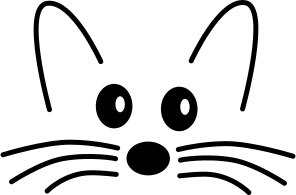
\includegraphics[width=1.4em]{squeak-logo}}}
\iftoshelse{
	\usepackage{marginnote}
		\renewcommand*{\marginfont}{\footnotesize}
	\newcommand{\vartriangleout}{\ifthenelse{\isodd{\thepage}}{\vartriangleright}{\vartriangleleft}}
	\newcommand{\dothisicon}{\fcolorbox{blue!65}{white}{\highlight{$\vartriangleout$}}}
	\newcommand{\dothis}[1]{%
		\noindent\par\noindent
		{\reversemarginpar
			\marginnote{\fcolorbox{blue!65}{white}{\highlight{$\vartriangleout$}}}}
		%\MarginLabel{do this}
		\noindent\emph{#1}
		\nopagebreak}
}{
	\newcommand{\dothisicon}{\raisebox{-.5ex}{
\includegraphics[height=1.2em]{pharo}}}
	\newcommand{\dothis}[1]{%
		\medskip
		\noindent\dothisicon
		\ifx#1\empty\else\quad\emph{#1}\fi
		\par\smallskip\nopagebreak}
}
%===> NEW VERSION <===
% NB: To use this in an individual chapter, you must set:
%\graphicspath{{figures/} {../figures/}}
% at the head of the chapter.  Don't forget the final /
%=============================================================
%:Reader hints (hint)
%
% Indicates a non-obvious consequence 
\newcommand{\hint}[1]{\vspace{1ex}\noindent\fbox{\textsc{Hint}} \emph{#1}}
%=================================================================
% graphics for Morphic handles
\newcommand{\grabHandle}{\raisebox{-0.2ex}{
\includegraphics[width=1em]{blackHandle}}}
\newcommand{\moveHandle}{\raisebox{-0.2ex}{
\includegraphics[width=1em]{moveHandle}}}
\newcommand{\debugHandle}{\raisebox{-0.2ex}{
\includegraphics[width=1em]{debugHandle}}}
%=============================================================
%:Highlighting Important stuff (doublebox)
%
% From Seaside book ...
\newsavebox{\SavedText}
\newlength{\InnerBoxRule}\setlength{\InnerBoxRule}{.75\fboxrule}
\newlength{\OuterBoxRule}\setlength{\OuterBoxRule}{1.5\fboxrule}
\newlength{\BoxSeparation}\setlength{\BoxSeparation}{1.5\fboxrule}
\addtolength{\BoxSeparation}{.5pt}
\newlength{\SaveBoxSep}\setlength{\SaveBoxSep}{2\fboxsep}
%
\newenvironment{doublebox}{\begin{lrbox}{\SavedText}
    \begin{minipage}{.75\textwidth}}
    {\end{minipage}\end{lrbox}\begin{center}
    \setlength{\fboxsep}{\BoxSeparation}\setlength{\fboxrule}{\OuterBoxRule}
    \fbox{\setlength{\fboxsep}{\SaveBoxSep}\setlength{\fboxrule}{\InnerBoxRule}%
      \fbox{\usebox{\SavedText}}}
  \end{center}}
% Use this:
\newcommand{\important}[1]{\begin{doublebox}#1\end{doublebox}}
%=============================================================
%:Section depth
\setcounter{secnumdepth}{2}
%% for this to happen start the file with
%\ifx\wholebook\relax\else
%% $Author$
% $Date$
% $Revision$

% HISTORY:
% 2006-10-31 - Oscar code macros
% ...

%=============================================================
% NB: documentclass must be set in main document.
% Allows book to be generated in multiple formats.
%=============================================================
%:Packages
\usepackage[T1]{fontenc}  %%%%%% really important to get the code directly in the text!
\usepackage{lmodern}
%\usepackage[scaled=0.85]{bookmanx} % needs another scale factor if used with \renewcommand{\sfdefault}{cmbr}
\usepackage{palatino}
\usepackage[scaled=0.85]{helvet}
\usepackage[protrusion,expansion=false]{microtype}
\usepackage{graphicx}
\usepackage{theorem}
\usepackage[english]{babel}
%%% ON: pdfsync breaks the use of p{width} for tabular columns!
%%\ifdefined\usepdfsync\usepackage{pdfsync}\fi % Requires texlive 2007
%=============================================================
%:More packages
%Stef should check which ones are used!
%\usepackage{picinpar}
%\usepackage{layout}
%\usepackage{color}
%\usepackage{enum}
%\usepackage{a4wide}
% \usepackage{fancyhdr}
\usepackage{ifthen}
\usepackage{float}
\usepackage{longtable}
\usepackage{makeidx}
\usepackage[nottoc]{tocbibind}
\usepackage{multicol}
\usepackage{booktabs}	% book-style tables
\usepackage{topcapt}	% enables \topcaption
\usepackage{multirow}
\usepackage{tabularx}
%\usepackage[bottom]{footmisc}
\usepackage{xspace}
\usepackage{alltt}
\usepackage{amssymb,textcomp}
\usepackage[usenames,dvipsnames]{color}
%\usepackage{colortbl}
\usepackage[hang]{subfigure}\makeatletter\def\p@subfigure{\thefigure\,}\makeatother
\usepackage{rotating}
\usepackage{enumitem}	% apb: allows more control over tags in enumerations
\usepackage{verbatim}     % for comment environment
\usepackage{varioref}	% for page references that work
\labelformat{footnote}{\thechapter--#1} % to distinguish citations from jurabib
\usepackage{needspace}
\usepackage{isodateo} % enable \isodate
\usepackage[newparttoc]{titlesec}
\usepackage{titletoc}
\usepackage{wrapfig}
\usepackage[
	super,
	citefull=first,
	authorformat={allreversed,and},
	titleformat={commasep,italic}
]{jurabib} % citations as footnotes
\usepackage[
	colorlinks=true,
	linkcolor=black,
	urlcolor=black,
	citecolor=black
]{hyperref}   % should come last
%=============================================================
%:PDF version
%%\pdfminorversion=3 % Set PDF to 1.3 for Lulu
%=============================================================
%:URL style
\makeatletter
\def\url@leostyle{%
  \@ifundefined{selectfont}{\def\UrlFont{\sf}}{\def\UrlFont{\sffamily}}}
\makeatother
% Now actually use the newly defined style.
\urlstyle{leo}
%=============================================================
%:Booleans
\newboolean{lulu}
\setboolean{lulu}{false}
\newcommand{\ifluluelse}[2]{\ifthenelse{\boolean{lulu}}{#1}{#2}}
%=============================================================
%:Names
\newcommand{\SUnit}{SUnit\xspace}
\newcommand{\sunit}{SUnit\xspace}
\newcommand{\xUnit}{$x$Unit\xspace}
\newcommand{\JUnit}{JUnit\xspace}
\newcommand{\st}{Smalltalk\xspace}
\newcommand{\pharo}{Pharo\xspace} % Use this, not \Pharo
%\newcommand{\sqmap}{SqueakMap\xspace}
\newcommand{\squeak}{Squeak\xspace} % use this, not \Squeak or \sq
\newcommand{\sqsrc}{SqueakSource\xspace}
\newcommand{\sbe}{\url{http://SqueakByExample.org}\xspace}
\newcommand{\pharoweb}{\url{http://pharo-project.org}\xspace}
\newcommand{\pbe}{\url{http://PharoByExample.org}\xspace}
\newcommand{\sba}{\url{http://SquareBracketAssociates.org}\xspace}
\newcommand{\bam}{\lct{Bounc\-ing\-Atoms\-Morph}\xspace}
%=============================================================
%:Markup macros for proof-reading
\usepackage[normalem]{ulem} % for \sout
\usepackage{xcolor}
\newcommand{\ra}{$\rightarrow$}
\newcommand{\ugh}[1]{\textcolor{red}{\uwave{#1}}} % please rephrase
\newcommand{\ins}[1]{\textcolor{blue}{\uline{#1}}} % please insert
\newcommand{\del}[1]{\textcolor{red}{\sout{#1}}} % please delete
\newcommand{\chg}[2]{\textcolor{red}{\sout{#1}}{\ra}\textcolor{blue}{\uline{#2}}} % please change
%=============================================================
%:Editorial comment macros
%\newcommand{\nnbb}[2]{
%    % \fbox{\bfseries\sffamily\scriptsize#1}
%    \fcolorbox{gray}{yellow}{\bfseries\sffamily\scriptsize#1}
%    {\sf\small$\blacktriangleright$\textit{#2}$\blacktriangleleft$}
%   }
\newcommand{\yellowbox}[1]{\fcolorbox{gray}{yellow}{\bfseries\sffamily\scriptsize#1}}
\newcommand{\triangles}[1]{{\sf\small$\blacktriangleright$\textit{#1}$\blacktriangleleft$}}
\newcommand{\nnbb}[2]{\yellowbox{#1} \triangles{#2}}
\newcommand{\fix}{\yellowbox{FIX!}}
\newcommand{\here}{\yellowbox{CONTINUE HERE!}}
% editor macros
\newcommand{\apl}[1]{\nnbb{Alain}{#1}} % Alain
\newcommand{\ab}[1]{\nnbb{Andrew}{#1}} % Black
\newcommand{\sd}[1]{\nnbb{St\'{e}f}{#1}} % Ducasse
\newcommand{\dc}[1]{\nnbb{DamienC}{#1}} % Ducasse
\newcommand{\md}[1]{\nnbb{Marcus}{#1}} % Denker
\newcommand{\on}[1]{\nnbb{Oscar}{#1}} % Nierstrasz
\newcommand{\damien}[1]{\nnbb{Damien}{#1}} % Pollet
\newcommand{\lr}[1]{\nnbb{Lukas}{#1}} % Renggli
\newcommand{\orla}[1]{\nnbb{Orla}{#1}} % Greevy
\newcommand{\alex}[1]{\nnbb{Alex}{#1}} % Bergel
\newcommand{\alx}[1]{\nnbb{Alex}{#1}} % Bergel
\newcommand{\dr}[1]{\nnbb{David}{#1}} % Roethlisberger
\newcommand{\ja}[1]{\nnbb{Jannik}{#1}} % Laval
\newcommand{\jr}[1]{\nnbb{Jorge}{#1}} % Ressia
\newcommand{\fp}[1]{\nnbb{Fabrizio}{#1}} % Perin
\newcommand{\michael}[1]{\nnbb{Michael}{#1}} % Davies
\newcommand{\ew}[1]{\nnbb{Erwann}{#1}} % Wernli
\newcommand{\mb}[1]{\nnbb{Martial}{#1}} % Boniou
\newcommand{\hw}[1]{\nnbb{Hernan}{#1}} % Wilkinson
%=============================================================
%:Abbreviation macros
\newcommand{\ie}{\emph{すなわち}、}
\newcommand{\eg}{\emph{例えば}、}
\newcommand{\etc}{などなど。}
%=============================================================
%:Cross reference macros
\newcommand{\charef}[1]{第~\ref{cha:#1}~章}
\newcommand{\secref}[1]{\ref{sec:#1}~節}
\newcommand{\figref}[1]{図~\ref{fig:#1}\xspace}
\newcommand{\Figref}[1]{図~\ref{fig:#1}\xspace}
\newcommand{\appref}[1]{付録~\ref{app:#1}\xspace}
\newcommand{\tabref}[1]{表~\ref{tab:#1}\xspace}
\newcommand{\faqref}[1]{FAQ~\ref{faq:#1}, p.~\pageref{faq:#1}\xspace}
% APB: I removed trailing \xspace commands from these macros because
% \xspace mostly doesn't work.  If you want a space after your
% references, type one!
% ON: xspace has always worked just fine for me!  Please leave them in.
%
\newcommand{\ruleref}[1]{\ref{rule:#1}\xspace}
%
\newcommand{\egref}[1]{example~\ref{eg:#1}\xspace}
\newcommand{\Egref}[1]{Example~\ref{eg:#1}\xspace}
%
\newcommand{\scrref}[1]{script~\ref{scr:#1}\xspace}
\newcommand{\Scrref}[1]{Script~\ref{scr:#1}\xspace}
\newcommand{\tscrref}[1]{the script~\ref{scr:#1}\xspace}
\newcommand{\Tscrref}[1]{The script~\ref{scr:#1}\xspace}
%
\newcommand{\mthref}[1]{method~\ref{mth:#1}\xspace}
\newcommand{\mthsref}[1]{methods~\ref{mth:#1}\xspace}
\newcommand{\Mthref}[1]{Method~\ref{mth:#1}\xspace}
\newcommand{\tmthref}[1]{the method~\ref{mth:#1}\xspace}
\newcommand{\Tmthref}[1]{The method~\ref{mth:#1}\xspace}
%
\newcommand{\clsref}[1]{class~\ref{cls:#1}\xspace}
\newcommand{\tclsref}[1]{the class~\ref{cls:#1}\xspace}
\newcommand{\Tclsref}[1]{The class~\ref{cls:#1}\xspace}

\newcommand{\chalabel}[1]{\label{cha:#1}}
\newcommand{\seclabel}[1]{\label{sec:#1}}
\newcommand{\figlabel}[1]{\label{fig:#1}}
\newcommand{\tablabel}[1]{\label{tab:#1}}
\newcommand{\rulelabel}[1]{\label{rule:#1}}
\newcommand{\eglabel}[1]{\label{eg:#1}}
\newcommand{\scrlabel}[1]{\label{scr:#1}}
\newcommand{\mthlabel}[1]{\label{mth:#1}}
\newcommand{\clslabel}[1]{\label{cls:#1}}
\newcommand{\faqlabel}[1]{\label{faq:#1}}
%=============================================================
%:Menu item macro
% for menu items, so we can change our minds on how to print them! (apb)
\definecolor{lightgray}{gray}{0.89}
\newcommand{\menu}[1]{{%
	\setlength{\fboxsep}{0pt}%
	\colorbox{lightgray}{{{\upshape\sffamily\strut \,#1\,}}}}}
\newcommand{\link}[1]{{%
	\fontfamily{lmr}\selectfont
 	\upshape{\sffamily \underline{#1}}}}
% For submenu items:
\newcommand{\go}{\,$\triangleright$\,}
% \newcommand{\go}{\,$\blacktriangleright$\,}
% For keyboard shortcuts:
%\newcommand{\short}[1]{\mbox{$\langle${\sc CMD}$\rangle$-#1}\xspace}
\newcommand{\short}[1]{\mbox{{\sc cmd}\hspace{0.08em}--\hspace{0.09em}#1}\xspace}
% For buttons:
\newcommand{\button}[1]{{%
	\setlength{\fboxsep}{0pt}%
	\fbox{{\upshape\sffamily\strut \,#1\,}}}}
% NB: The button macro does not work within captions -- incompatible with xcolor package :-(
\newcommand{\toolsflap}{\textit{Tools} flap\xspace}
%=============================================================
%:Mouse clicks
\newcommand{\click}{click\xspace} % RED
\newcommand{\actclick}{action-click\xspace} % YELLOW
\newcommand{\metaclick}{meta-click\xspace} % BLUE
\newcommand{\Click}{Click\xspace} % RED
\newcommand{\Actclick}{Action-click\xspace} % YELLOW
\newcommand{\Metaclick}{Meta-click\xspace} % BLUE
%=============================================================
%:ToSh macros
\newboolean{tosh}
\setboolean{tosh}{false}
\newcommand{\iftoshelse}[2]{\ifthenelse{\boolean{tosh}}{#1}{#2}}
%=============================================================
%:ToSh colors
%\newcommand{\highlightcolor}{\color{blue!65}}
%\newcommand{\boxcolor}{\color{gray!25}}
\newcommand{\highlight}[1]{\textcolor{blue!65}{#1}}
%\newcommand{\codecolor}{\color{blue!65}}
%%\setlength{\fboxrule}{2pt}
%\newcommand{\asPict}[1]{%
%	{\Large\highlight{#1}}}
%=============================================================
%:Reader cues (do this)
%
% Indicate something the reader should try out.
% \newcommand{\dothisicon}{\raisebox{-.5ex}{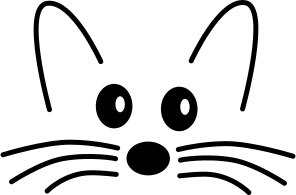
\includegraphics[width=1.4em]{squeak-logo}}}
\iftoshelse{
	\usepackage{marginnote}
		\renewcommand*{\marginfont}{\footnotesize}
	\newcommand{\vartriangleout}{\ifthenelse{\isodd{\thepage}}{\vartriangleright}{\vartriangleleft}}
	\newcommand{\dothisicon}{\fcolorbox{blue!65}{white}{\highlight{$\vartriangleout$}}}
	\newcommand{\dothis}[1]{%
		\noindent\par\noindent
		{\reversemarginpar
			\marginnote{\fcolorbox{blue!65}{white}{\highlight{$\vartriangleout$}}}}
		%\MarginLabel{do this}
		\noindent\emph{#1}
		\nopagebreak}
}{
	\newcommand{\dothisicon}{\raisebox{-.5ex}{
\includegraphics[height=1.2em]{pharo}}}
	\newcommand{\dothis}[1]{%
		\medskip
		\noindent\dothisicon
		\ifx#1\empty\else\quad\emph{#1}\fi
		\par\smallskip\nopagebreak}
}
%===> NEW VERSION <===
% NB: To use this in an individual chapter, you must set:
%\graphicspath{{figures/} {../figures/}}
% at the head of the chapter.  Don't forget the final /
%=============================================================
%:Reader hints (hint)
%
% Indicates a non-obvious consequence 
\newcommand{\hint}[1]{\vspace{1ex}\noindent\fbox{\textsc{Hint}} \emph{#1}}
%=================================================================
% graphics for Morphic handles
\newcommand{\grabHandle}{\raisebox{-0.2ex}{
\includegraphics[width=1em]{blackHandle}}}
\newcommand{\moveHandle}{\raisebox{-0.2ex}{
\includegraphics[width=1em]{moveHandle}}}
\newcommand{\debugHandle}{\raisebox{-0.2ex}{
\includegraphics[width=1em]{debugHandle}}}
%=============================================================
%:Highlighting Important stuff (doublebox)
%
% From Seaside book ...
\newsavebox{\SavedText}
\newlength{\InnerBoxRule}\setlength{\InnerBoxRule}{.75\fboxrule}
\newlength{\OuterBoxRule}\setlength{\OuterBoxRule}{1.5\fboxrule}
\newlength{\BoxSeparation}\setlength{\BoxSeparation}{1.5\fboxrule}
\addtolength{\BoxSeparation}{.5pt}
\newlength{\SaveBoxSep}\setlength{\SaveBoxSep}{2\fboxsep}
%
\newenvironment{doublebox}{\begin{lrbox}{\SavedText}
    \begin{minipage}{.75\textwidth}}
    {\end{minipage}\end{lrbox}\begin{center}
    \setlength{\fboxsep}{\BoxSeparation}\setlength{\fboxrule}{\OuterBoxRule}
    \fbox{\setlength{\fboxsep}{\SaveBoxSep}\setlength{\fboxrule}{\InnerBoxRule}%
      \fbox{\usebox{\SavedText}}}
  \end{center}}
% Use this:
\newcommand{\important}[1]{\begin{doublebox}#1\end{doublebox}}
%=============================================================
%:Section depth
\setcounter{secnumdepth}{2}
%% for this to happen start the file with
%\ifx\wholebook\relax\else
%% $Author$
% $Date$
% $Revision$

% HISTORY:
% 2006-10-31 - Oscar code macros
% ...

%=============================================================
% NB: documentclass must be set in main document.
% Allows book to be generated in multiple formats.
%=============================================================
%:Packages
\usepackage[T1]{fontenc}  %%%%%% really important to get the code directly in the text!
\usepackage{lmodern}
%\usepackage[scaled=0.85]{bookmanx} % needs another scale factor if used with \renewcommand{\sfdefault}{cmbr}
\usepackage{palatino}
\usepackage[scaled=0.85]{helvet}
\usepackage[protrusion,expansion=false]{microtype}
\usepackage{graphicx}
\usepackage{theorem}
\usepackage[english]{babel}
%%% ON: pdfsync breaks the use of p{width} for tabular columns!
%%\ifdefined\usepdfsync\usepackage{pdfsync}\fi % Requires texlive 2007
%=============================================================
%:More packages
%Stef should check which ones are used!
%\usepackage{picinpar}
%\usepackage{layout}
%\usepackage{color}
%\usepackage{enum}
%\usepackage{a4wide}
% \usepackage{fancyhdr}
\usepackage{ifthen}
\usepackage{float}
\usepackage{longtable}
\usepackage{makeidx}
\usepackage[nottoc]{tocbibind}
\usepackage{multicol}
\usepackage{booktabs}	% book-style tables
\usepackage{topcapt}	% enables \topcaption
\usepackage{multirow}
\usepackage{tabularx}
%\usepackage[bottom]{footmisc}
\usepackage{xspace}
\usepackage{alltt}
\usepackage{amssymb,textcomp}
\usepackage[usenames,dvipsnames]{color}
%\usepackage{colortbl}
\usepackage[hang]{subfigure}\makeatletter\def\p@subfigure{\thefigure\,}\makeatother
\usepackage{rotating}
\usepackage{enumitem}	% apb: allows more control over tags in enumerations
\usepackage{verbatim}     % for comment environment
\usepackage{varioref}	% for page references that work
\labelformat{footnote}{\thechapter--#1} % to distinguish citations from jurabib
\usepackage{needspace}
\usepackage{isodateo} % enable \isodate
\usepackage[newparttoc]{titlesec}
\usepackage{titletoc}
\usepackage{wrapfig}
\usepackage[
	super,
	citefull=first,
	authorformat={allreversed,and},
	titleformat={commasep,italic}
]{jurabib} % citations as footnotes
\usepackage[
	colorlinks=true,
	linkcolor=black,
	urlcolor=black,
	citecolor=black
]{hyperref}   % should come last
%=============================================================
%:PDF version
%%\pdfminorversion=3 % Set PDF to 1.3 for Lulu
%=============================================================
%:URL style
\makeatletter
\def\url@leostyle{%
  \@ifundefined{selectfont}{\def\UrlFont{\sf}}{\def\UrlFont{\sffamily}}}
\makeatother
% Now actually use the newly defined style.
\urlstyle{leo}
%=============================================================
%:Booleans
\newboolean{lulu}
\setboolean{lulu}{false}
\newcommand{\ifluluelse}[2]{\ifthenelse{\boolean{lulu}}{#1}{#2}}
%=============================================================
%:Names
\newcommand{\SUnit}{SUnit\xspace}
\newcommand{\sunit}{SUnit\xspace}
\newcommand{\xUnit}{$x$Unit\xspace}
\newcommand{\JUnit}{JUnit\xspace}
\newcommand{\st}{Smalltalk\xspace}
\newcommand{\pharo}{Pharo\xspace} % Use this, not \Pharo
%\newcommand{\sqmap}{SqueakMap\xspace}
\newcommand{\squeak}{Squeak\xspace} % use this, not \Squeak or \sq
\newcommand{\sqsrc}{SqueakSource\xspace}
\newcommand{\sbe}{\url{http://SqueakByExample.org}\xspace}
\newcommand{\pharoweb}{\url{http://pharo-project.org}\xspace}
\newcommand{\pbe}{\url{http://PharoByExample.org}\xspace}
\newcommand{\sba}{\url{http://SquareBracketAssociates.org}\xspace}
\newcommand{\bam}{\lct{Bounc\-ing\-Atoms\-Morph}\xspace}
%=============================================================
%:Markup macros for proof-reading
\usepackage[normalem]{ulem} % for \sout
\usepackage{xcolor}
\newcommand{\ra}{$\rightarrow$}
\newcommand{\ugh}[1]{\textcolor{red}{\uwave{#1}}} % please rephrase
\newcommand{\ins}[1]{\textcolor{blue}{\uline{#1}}} % please insert
\newcommand{\del}[1]{\textcolor{red}{\sout{#1}}} % please delete
\newcommand{\chg}[2]{\textcolor{red}{\sout{#1}}{\ra}\textcolor{blue}{\uline{#2}}} % please change
%=============================================================
%:Editorial comment macros
%\newcommand{\nnbb}[2]{
%    % \fbox{\bfseries\sffamily\scriptsize#1}
%    \fcolorbox{gray}{yellow}{\bfseries\sffamily\scriptsize#1}
%    {\sf\small$\blacktriangleright$\textit{#2}$\blacktriangleleft$}
%   }
\newcommand{\yellowbox}[1]{\fcolorbox{gray}{yellow}{\bfseries\sffamily\scriptsize#1}}
\newcommand{\triangles}[1]{{\sf\small$\blacktriangleright$\textit{#1}$\blacktriangleleft$}}
\newcommand{\nnbb}[2]{\yellowbox{#1} \triangles{#2}}
\newcommand{\fix}{\yellowbox{FIX!}}
\newcommand{\here}{\yellowbox{CONTINUE HERE!}}
% editor macros
\newcommand{\apl}[1]{\nnbb{Alain}{#1}} % Alain
\newcommand{\ab}[1]{\nnbb{Andrew}{#1}} % Black
\newcommand{\sd}[1]{\nnbb{St\'{e}f}{#1}} % Ducasse
\newcommand{\dc}[1]{\nnbb{DamienC}{#1}} % Ducasse
\newcommand{\md}[1]{\nnbb{Marcus}{#1}} % Denker
\newcommand{\on}[1]{\nnbb{Oscar}{#1}} % Nierstrasz
\newcommand{\damien}[1]{\nnbb{Damien}{#1}} % Pollet
\newcommand{\lr}[1]{\nnbb{Lukas}{#1}} % Renggli
\newcommand{\orla}[1]{\nnbb{Orla}{#1}} % Greevy
\newcommand{\alex}[1]{\nnbb{Alex}{#1}} % Bergel
\newcommand{\alx}[1]{\nnbb{Alex}{#1}} % Bergel
\newcommand{\dr}[1]{\nnbb{David}{#1}} % Roethlisberger
\newcommand{\ja}[1]{\nnbb{Jannik}{#1}} % Laval
\newcommand{\jr}[1]{\nnbb{Jorge}{#1}} % Ressia
\newcommand{\fp}[1]{\nnbb{Fabrizio}{#1}} % Perin
\newcommand{\michael}[1]{\nnbb{Michael}{#1}} % Davies
\newcommand{\ew}[1]{\nnbb{Erwann}{#1}} % Wernli
\newcommand{\mb}[1]{\nnbb{Martial}{#1}} % Boniou
\newcommand{\hw}[1]{\nnbb{Hernan}{#1}} % Wilkinson
%=============================================================
%:Abbreviation macros
\newcommand{\ie}{\emph{すなわち}、}
\newcommand{\eg}{\emph{例えば}、}
\newcommand{\etc}{などなど。}
%=============================================================
%:Cross reference macros
\newcommand{\charef}[1]{第~\ref{cha:#1}~章}
\newcommand{\secref}[1]{\ref{sec:#1}~節}
\newcommand{\figref}[1]{図~\ref{fig:#1}\xspace}
\newcommand{\Figref}[1]{図~\ref{fig:#1}\xspace}
\newcommand{\appref}[1]{付録~\ref{app:#1}\xspace}
\newcommand{\tabref}[1]{表~\ref{tab:#1}\xspace}
\newcommand{\faqref}[1]{FAQ~\ref{faq:#1}, p.~\pageref{faq:#1}\xspace}
% APB: I removed trailing \xspace commands from these macros because
% \xspace mostly doesn't work.  If you want a space after your
% references, type one!
% ON: xspace has always worked just fine for me!  Please leave them in.
%
\newcommand{\ruleref}[1]{\ref{rule:#1}\xspace}
%
\newcommand{\egref}[1]{example~\ref{eg:#1}\xspace}
\newcommand{\Egref}[1]{Example~\ref{eg:#1}\xspace}
%
\newcommand{\scrref}[1]{script~\ref{scr:#1}\xspace}
\newcommand{\Scrref}[1]{Script~\ref{scr:#1}\xspace}
\newcommand{\tscrref}[1]{the script~\ref{scr:#1}\xspace}
\newcommand{\Tscrref}[1]{The script~\ref{scr:#1}\xspace}
%
\newcommand{\mthref}[1]{method~\ref{mth:#1}\xspace}
\newcommand{\mthsref}[1]{methods~\ref{mth:#1}\xspace}
\newcommand{\Mthref}[1]{Method~\ref{mth:#1}\xspace}
\newcommand{\tmthref}[1]{the method~\ref{mth:#1}\xspace}
\newcommand{\Tmthref}[1]{The method~\ref{mth:#1}\xspace}
%
\newcommand{\clsref}[1]{class~\ref{cls:#1}\xspace}
\newcommand{\tclsref}[1]{the class~\ref{cls:#1}\xspace}
\newcommand{\Tclsref}[1]{The class~\ref{cls:#1}\xspace}

\newcommand{\chalabel}[1]{\label{cha:#1}}
\newcommand{\seclabel}[1]{\label{sec:#1}}
\newcommand{\figlabel}[1]{\label{fig:#1}}
\newcommand{\tablabel}[1]{\label{tab:#1}}
\newcommand{\rulelabel}[1]{\label{rule:#1}}
\newcommand{\eglabel}[1]{\label{eg:#1}}
\newcommand{\scrlabel}[1]{\label{scr:#1}}
\newcommand{\mthlabel}[1]{\label{mth:#1}}
\newcommand{\clslabel}[1]{\label{cls:#1}}
\newcommand{\faqlabel}[1]{\label{faq:#1}}
%=============================================================
%:Menu item macro
% for menu items, so we can change our minds on how to print them! (apb)
\definecolor{lightgray}{gray}{0.89}
\newcommand{\menu}[1]{{%
	\setlength{\fboxsep}{0pt}%
	\colorbox{lightgray}{{{\upshape\sffamily\strut \,#1\,}}}}}
\newcommand{\link}[1]{{%
	\fontfamily{lmr}\selectfont
 	\upshape{\sffamily \underline{#1}}}}
% For submenu items:
\newcommand{\go}{\,$\triangleright$\,}
% \newcommand{\go}{\,$\blacktriangleright$\,}
% For keyboard shortcuts:
%\newcommand{\short}[1]{\mbox{$\langle${\sc CMD}$\rangle$-#1}\xspace}
\newcommand{\short}[1]{\mbox{{\sc cmd}\hspace{0.08em}--\hspace{0.09em}#1}\xspace}
% For buttons:
\newcommand{\button}[1]{{%
	\setlength{\fboxsep}{0pt}%
	\fbox{{\upshape\sffamily\strut \,#1\,}}}}
% NB: The button macro does not work within captions -- incompatible with xcolor package :-(
\newcommand{\toolsflap}{\textit{Tools} flap\xspace}
%=============================================================
%:Mouse clicks
\newcommand{\click}{click\xspace} % RED
\newcommand{\actclick}{action-click\xspace} % YELLOW
\newcommand{\metaclick}{meta-click\xspace} % BLUE
\newcommand{\Click}{Click\xspace} % RED
\newcommand{\Actclick}{Action-click\xspace} % YELLOW
\newcommand{\Metaclick}{Meta-click\xspace} % BLUE
%=============================================================
%:ToSh macros
\newboolean{tosh}
\setboolean{tosh}{false}
\newcommand{\iftoshelse}[2]{\ifthenelse{\boolean{tosh}}{#1}{#2}}
%=============================================================
%:ToSh colors
%\newcommand{\highlightcolor}{\color{blue!65}}
%\newcommand{\boxcolor}{\color{gray!25}}
\newcommand{\highlight}[1]{\textcolor{blue!65}{#1}}
%\newcommand{\codecolor}{\color{blue!65}}
%%\setlength{\fboxrule}{2pt}
%\newcommand{\asPict}[1]{%
%	{\Large\highlight{#1}}}
%=============================================================
%:Reader cues (do this)
%
% Indicate something the reader should try out.
% \newcommand{\dothisicon}{\raisebox{-.5ex}{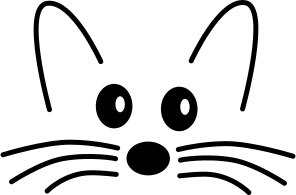
\includegraphics[width=1.4em]{squeak-logo}}}
\iftoshelse{
	\usepackage{marginnote}
		\renewcommand*{\marginfont}{\footnotesize}
	\newcommand{\vartriangleout}{\ifthenelse{\isodd{\thepage}}{\vartriangleright}{\vartriangleleft}}
	\newcommand{\dothisicon}{\fcolorbox{blue!65}{white}{\highlight{$\vartriangleout$}}}
	\newcommand{\dothis}[1]{%
		\noindent\par\noindent
		{\reversemarginpar
			\marginnote{\fcolorbox{blue!65}{white}{\highlight{$\vartriangleout$}}}}
		%\MarginLabel{do this}
		\noindent\emph{#1}
		\nopagebreak}
}{
	\newcommand{\dothisicon}{\raisebox{-.5ex}{
\includegraphics[height=1.2em]{pharo}}}
	\newcommand{\dothis}[1]{%
		\medskip
		\noindent\dothisicon
		\ifx#1\empty\else\quad\emph{#1}\fi
		\par\smallskip\nopagebreak}
}
%===> NEW VERSION <===
% NB: To use this in an individual chapter, you must set:
%\graphicspath{{figures/} {../figures/}}
% at the head of the chapter.  Don't forget the final /
%=============================================================
%:Reader hints (hint)
%
% Indicates a non-obvious consequence 
\newcommand{\hint}[1]{\vspace{1ex}\noindent\fbox{\textsc{Hint}} \emph{#1}}
%=================================================================
% graphics for Morphic handles
\newcommand{\grabHandle}{\raisebox{-0.2ex}{
\includegraphics[width=1em]{blackHandle}}}
\newcommand{\moveHandle}{\raisebox{-0.2ex}{
\includegraphics[width=1em]{moveHandle}}}
\newcommand{\debugHandle}{\raisebox{-0.2ex}{
\includegraphics[width=1em]{debugHandle}}}
%=============================================================
%:Highlighting Important stuff (doublebox)
%
% From Seaside book ...
\newsavebox{\SavedText}
\newlength{\InnerBoxRule}\setlength{\InnerBoxRule}{.75\fboxrule}
\newlength{\OuterBoxRule}\setlength{\OuterBoxRule}{1.5\fboxrule}
\newlength{\BoxSeparation}\setlength{\BoxSeparation}{1.5\fboxrule}
\addtolength{\BoxSeparation}{.5pt}
\newlength{\SaveBoxSep}\setlength{\SaveBoxSep}{2\fboxsep}
%
\newenvironment{doublebox}{\begin{lrbox}{\SavedText}
    \begin{minipage}{.75\textwidth}}
    {\end{minipage}\end{lrbox}\begin{center}
    \setlength{\fboxsep}{\BoxSeparation}\setlength{\fboxrule}{\OuterBoxRule}
    \fbox{\setlength{\fboxsep}{\SaveBoxSep}\setlength{\fboxrule}{\InnerBoxRule}%
      \fbox{\usebox{\SavedText}}}
  \end{center}}
% Use this:
\newcommand{\important}[1]{\begin{doublebox}#1\end{doublebox}}
%=============================================================
%:Section depth
\setcounter{secnumdepth}{2}
%% for this to happen start the file with
%\ifx\wholebook\relax\else
%\input{../common.tex}
%\begin{document}
%\fi
% and terminate by
% \ifx\wholebook\relax\else\end{document}\fi

\DeclareGraphicsExtensions{.pdf, .jpg, .png}
%=============================================================
%:PDF setup
\hypersetup{
%   a4paper,
%   pdfstartview=FitV,
%   colorlinks,
%   linkcolor=darkblue,
%   citecolor=darkblue,
   pdftitle={Pharo by Example},
   pdfauthor={Andrew P. Black, St\'ephane Ducasse,	Oscar Nierstrasz,
Damien Pollet},
   pdfkeywords={Smalltalk, Squeak, Object-Oriented Programming, OOP},
   pdfsubject={Computer Science}
}
%=============================================================
%:Page layout and appearance
%
% \renewcommand{\headrulewidth}{0pt}
\renewcommand{\chaptermark}[1]{\markboth{#1}{}}
\renewcommand{\sectionmark}[1]{\markright{\thesection\ #1}}
\renewpagestyle{plain}[\small\itshape]{%
	\setheadrule{0pt}%
	\sethead[][][]{}{}{}%
	\setfoot[][][]{}{}{}}
\renewpagestyle{headings}[\small\itshape]{%
	\setheadrule{0pt}%
	\setmarks{chapter}{section}%
	\sethead[\thepage][][\chaptertitle]{\sectiontitle}{}{\thepage}%
	\setfoot[][][]{}{}{}}
%=============================================================
%:Title section setup and TOC numbering depth
\setcounter{secnumdepth}{1}
\setcounter{tocdepth}{1}
\titleformat{\part}[display]{\centering}{\huge\partname\ \thepart}{1em}{\Huge\textbf}[]
\titleformat{\chapter}[display]{}{\huge\chaptertitlename\ \thechapter}{1em}{\Huge\raggedright\textbf}[]
\titlecontents{part}[3pc]{%
		\pagebreak[2]\addvspace{1em plus.4em minus.2em}%
		\leavevmode\large\bfseries}
	{\contentslabel{3pc}}{\hspace*{-3pc}}
	{}[\nopagebreak]
\titlecontents{chapter}[3pc]{%
		\pagebreak[0]\addvspace{1em plus.2em minus.2em}%
		\leavevmode\bfseries}
	{\contentslabel{3pc}}{}
	{\hfill\contentspage}[\nopagebreak]
\dottedcontents{section}[3pc]{}{3pc}{1pc}
\dottedcontents{subsection}[3pc]{}{0pc}{1pc}
% \dottedcontents{subsection}[4.5em]{}{0pt}{1pc}
% Make \cleardoublepage insert really blank pages http://www.tex.ac.uk/cgi-bin/texfaq2html?label=reallyblank
\let\origdoublepage\cleardoublepage
\newcommand{\clearemptydoublepage}{%
  \clearpage
  {\pagestyle{empty}\origdoublepage}}
\let\cleardoublepage\clearemptydoublepage % see http://www.tex.ac.uk/cgi-bin/texfaq2html?label=patch
%=============================================================
%:FAQ macros (for FAQ chapter)
\newtheorem{faq}{FAQ}
\newcommand{\answer}{\paragraph{Answer}\ }
%=============================================================
%:Listings package configuration
% \newcommand{\caret}{\makebox{\raisebox{0.4ex}{\footnotesize{$\wedge$}}}}
\newcommand{\caret}{\^\,}
\newcommand{\escape}{{\sf \textbackslash}}
\definecolor{source}{gray}{0.95}
\usepackage{listings}
\lstdefinelanguage{Smalltalk}{
%  morekeywords={self,super,true,false,nil,thisContext}, % This is overkill
  morestring=[d]',
  morecomment=[s]{"}{"},
  alsoletter={\#:},
  escapechar={!},
  literate=
    {BANG}{!}1
    {CARET}{\^}1
    {UNDERSCORE}{\_}1
    {\\st}{Smalltalk}9 % convenience -- in case \st occurs in code
    % {'}{{\textquotesingle}}1 % replaced by upquote=true in \lstset
    {_}{{$\leftarrow$}}1
    {>>>}{{\sep}}1
    {^}{{$\uparrow$}}1
    {~}{{$\sim$}}1
    {-}{{\texttt{-}}}1 %{\textminus}}1 %{-}{\hspace{-0.13em}}{-}}1  % the goal is to make - the same width as +
    % {+}{\sf+}1 %{\raisebox{0.08ex}{+}}}1      % and to raise + off the baseline to match -
    {-->}{{\quad$\longrightarrow$\quad}}3
	, % Don't forget the comma at the end!
  tabsize=4
}[keywords,comments,strings]

\lstset{language=Smalltalk,
	basicstyle=\sffamily,
	keywordstyle=\color{black}\bfseries,
	% stringstyle=\ttfamily, % Ugly! do we really want this? -- on
	mathescape=true,
	showstringspaces=false,
	keepspaces=true,
	breaklines=true,
	breakautoindent=true,
	backgroundcolor=\color{source},
	lineskip={-1pt}, % Ugly hack
	upquote=true, % straight quote; requires textcomp package
	columns=fullflexible} % no fixed width fonts
% In-line code (literal)
% Normally use this for all in-line code:
\newcommand{\ct}{\lstinline[mathescape=false,backgroundcolor=\color{white},basicstyle={\sffamily\upshape}]}
% apb 2007.8.28 added the \upshape declaration to avoid getting italicized code in \dothis{ } sections.
% In-line code (latex enabled)
% Use this only in special situations where \ct does not work
% (within section headings ...):
\newcommand{\lct}[1]{{\textsf{\textup{#1}}}}
% Use these for system categories and protocols:
\newcommand{\scat}[1]{\emph{\textsf{#1}}\xspace}
\newcommand{\pkg}[1]{\emph{\textsf{#1}}\xspace}
\newcommand{\prot}[1]{\emph{\textsf{#1}}\xspace}
% Code environments
% NB: the arg is for tests
% Only code and example environments may be tests
\lstnewenvironment{code}[1]{%
	\lstset{%
		% frame=lines,
		frame=single,
		framerule=0pt,
		mathescape=false
	}
}{}
\def\ignoredollar#1{}
%=============================================================
%:Code environments (method, script ...)
% NB: the third arg is for tests
% Only code and example environments may be tests
\lstnewenvironment{example}[3][defaultlabel]{%
	\renewcommand{\lstlistingname}{Example}%
	\lstset{
		% frame=lines,
		frame=single,
		framerule=0pt,
		mathescape=false,
		caption={\emph{#2}},
		label={eg:#1}
	}
}{}
\lstnewenvironment{script}[2][defaultlabel]{%
\renewcommand{\lstlistingname}{Script}%
	\lstset{
		% frame=lines,
		frame=single,
		framerule=0pt,
		mathescape=false,
		name={Script},
		caption={\emph{#2}},
		label={scr:#1}
	}
}{}
\lstnewenvironment{method}[2][defaultlabel]{%
	\renewcommand{\lstlistingname}{Method}%
	\lstset{
		% frame=lines,
		frame=single,
		framerule=0pt,
		mathescape=false,
		name={Method},
		caption={\emph{#2}},
		label={mth:#1}
	}
}{}
\lstnewenvironment{methods}[2][defaultlabel]{% just for multiple methods at once
	\renewcommand{\lstlistingname}{Methods}%
	\lstset{
		% frame=lines,
		frame=single,
		framerule=0pt,
		mathescape=false,
		name={Method},
		caption={\emph{#2}},
		label={mth:#1}
	}
}{}
\lstnewenvironment{numMethod}[2][defaultlabel]{%
	\renewcommand{\lstlistingname}{Method}%
	\lstset{
		numbers=left,
		numberstyle={\tiny\sffamily},
		% frame=lines,
		frame=single,
		framerule=0pt,
		mathescape=false,
		name={Method},
		caption={\emph{#2}},
		label={mth:#1}
	}
}{}
\lstnewenvironment{classdef}[2][defaultlabel]{%
	\renewcommand{\lstlistingname}{Class}%
	\lstset{
		% frame=lines,
		frame=single,
		framerule=0pt,
		mathescape=false,
		name={Class},
		caption={\emph{#2}},
		label={cls:#1}
	}
}{}
%=============================================================
%:Reserving space
% Usually need one more line than the actual lines of code
\newcommand{\needlines}[1]{\Needspace{#1\baselineskip}}
%=============================================================
%:Indexing macros
% Macros ending with "ind" generate text as well as an index entry
% Macros ending with "index" *only* generate an index entry
\newcommand{\ind}[1]{\index{#1}#1\xspace} % plain text
\newcommand{\subind}[2]{\index{#1!#2}#2\xspace} % show #2, subindex under #1
\newcommand{\emphind}[1]{\index{#1}\emph{#1}\xspace} % emph #1
\newcommand{\emphsubind}[2]{\index{#1!#2}\emph{#2}\xspace} % show emph #2, subindex inder #1
\newcommand{\scatind}[1]{\index{#1@\textsf{#1} (category)}\scat{#1}} % category
\newcommand{\pkgind}[1]{\index{#1@\textsf{#1} (package)}\pkg{#1}} % package
\newcommand{\protind}[1]{\index{#1@\textsf{#1} (protocol)}\prot{#1}} % protocol
\newcommand{\clsind}[1]{\index{#1@\textsf{#1} (class)}\ct{#1}\xspace}
% \newcommand{\clsind}[1]{\index{#1!\#@(class)}\ct{#1}\xspace} % class
\newcommand{\clsindplural}[1]{\index{#1!\#@(class)}\ct{#1}s\xspace} % class
\newcommand{\cvind}[1]{\index{#1@\textsf{#1} (class variable)}\ct{#1}\xspace} % class var
\newcommand{\glbind}[1]{\index{#1@\textsf{#1} (global)}\ct{#1}\xspace} % global
\newcommand{\patind}[1]{\index{#1@#1 (pattern)}\ct{#1}\xspace} % pattern
\newcommand{\pvind}[1]{\index{#1@\textsf{#1} (pseudo variable)}\ct{#1}\xspace} % pseudo var
\newcommand{\clsmthind}[2]{\index{#1!#2@\ct{#2}}\ct{#1>>>#2}\xspace} % class + method name
\newcommand{\mthind}[2]{\index{#1!#2@\ct{#2}}\ct{#2}\xspace} % show method name only
\newcommand{\lmthind}[2]{\index{#1!#2@\ct{#2}}\lct{#2}\xspace} % show method name only
\newcommand{\cmind}[2]{\index{#1!#2@\ct{#2}}\ct{#1>>>#2}\xspace} % show class>>method
\newcommand{\lcmind}[2]{\index{#1!#2@\ct{#2}}\lct{#1>>>#2}\xspace} % show class>>method
\newcommand{\toolsflapind}{\index{Tools flap}\toolsflap} % index tools flap
% The following only generate an index entry:
% \newcommand{\clsindex}[1]{\index{#1@\textsf{#1} (class)}}
\newcommand{\clsindex}[1]{\index{#1!\#@(class)}} % class
\newcommand{\mthindex}[2]{\index{#1!#2@\ct{#2}}} % method
\newcommand{\cmindex}[2]{\index{#1!#2@\ct{#2}}} % class>>method
\newcommand{\cvindex}[1]{\index{#1@\textsf{#1} (class variable)}} % class var
\newcommand{\glbindex}[1]{\index{#1@\textsf{#1} (global)}}% global
\newcommand{\pvindex}[1]{\index{#1@\textsf{#1} (pseudo variable)}}% pseudo var
\newcommand{\seeindex}[2]{\index{#1|see{#2}}} % #1, see #2
\newcommand{\scatindex}[1]{\index{#1@\textsf{#1} (category)}} % category
\newcommand{\pkgindex}[1]{\index{#1@\textsf{#1} (package)}} % package
\newcommand{\protindex}[1]{\index{#1@\textsf{#1} (protocol)}} % protocol
% How can we have the main entry page numbers in bold yet not break the hyperlink?
\newcommand{\boldidx}[1]{{\bf #1}} % breaks hyperlink
%\newcommand{\indmain}[1]{\index{#1|boldidx}#1\xspace} % plain text, main entry
%\newcommand{\emphsubindmain}[2]{\index{#1!#2|boldidx}\emph{#2}\xspace} % subindex, main entry
%\newcommand{\subindmain}[2]{\index{#1!#2|boldidx}#2\xspace} % subindex, main entry
%\newcommand{\clsindmain}[1]{\index{#1@\textsf{#1} (class)|boldidx}\ct{#1}\xspace}
%\newcommand{\clsindmain}[1]{\index{#1!\#@(class)|boldidx}\ct{#1}\xspace} % class main
%\newcommand{\indexmain}[1]{\index{#1|boldidx}} % main index entry only
\newcommand{\indmain}[1]{\index{#1}#1\xspace} % The main index entry for this item
\newcommand{\emphsubindmain}[2]{\index{#1!#2}\emph{#2}\xspace} % subindex, main entry
\newcommand{\subindmain}[2]{\index{#1!#2}#2\xspace} % subindex, main entry
%\newcommand{\clsindmain}[1]{\index{#1@\textsf{#1} (class)}\ct{#1}\xspace}
\newcommand{\clsindmain}[1]{\index{#1!\#@(class)}\ct{#1}\xspace} % class main
\newcommand{\clsindexmain}[1]{\index{#1!\#@(class)}} % class main index only
\newcommand{\indexmain}[1]{\index{#1}} 
%=============================================================
%:Code macros
% some constants
\newcommand{\codesize}{\small}
\newcommand{\codefont}{\sffamily}
%\newcommand{\cat}[1]{\textit{In category #1}}%%To remove later
\newlength{\scriptindent}
\setlength{\scriptindent}{.3cm}
%% Method presentation constants
\newlength{\methodindent}
\newlength{\methodwordlength}
\newlength{\aftermethod}
\setlength{\methodindent}{0.2cm}
\settowidth{\methodwordlength}{\ M\'ethode\ }
%=============================================================
%:Smalltalk macros
%\newcommand{\sep}{{$\gg$}}
\newcommand{\sep}{\mbox{>>}}
\newcommand{\self}{\lct{self}\xspace}
\newcommand{\super}{\lct{super}\xspace}
\newcommand{\nil}{\lct{nil}\xspace}
%=============================================================
% be less conservative about float placement
% these commands are from http://www.tex.ac.uk/cgi-bin/texfaq2html?label=floats
\renewcommand{\topfraction}{.9}
\renewcommand{\bottomfraction}{.9}
\renewcommand{\textfraction}{.1}
\renewcommand{\floatpagefraction}{.85}
\renewcommand{\dbltopfraction}{.66}
\renewcommand{\dblfloatpagefraction}{.85}
\setcounter{topnumber}{9}
\setcounter{bottomnumber}{9}
\setcounter{totalnumber}{20}
\setcounter{dbltopnumber}{9}
%=============================================================
% Give information from each chapter's author
\newcommand{\contact}[2]{\textbf{#1} \textsf{(#2)}}

\newcommand{\chapterauthor}[1]{\emph{with the participation of:\\#1}\\}

\newcommand{\authornoury}{\contact{Noury Bouraqadi}{bouraqadi@gmail.com}}
\newcommand{\authordamienc}{\contact{Damien Cassou}{damien.cassou@gmail.com}}
\newcommand{\authoroscar}{\contact{Oscar Nierstrasz}{oscar.nierstrasz@acm.org}}
\newcommand{\authorsteph}{\contact{St\'ephane Ducasse}{stephane.ducasse@inria.fr}}
\newcommand{\authoralex}{\contact{Alexandre Bergel}{alexandre@bergel.eu}}
\newcommand{\authorolivier}{\contact{Olivier Auverlot}{olivier.auverlot@inria.fr}}
\newcommand{\authornicolas}{\contact{Nicolas Cellier}{ncellier@ifrance.com}}
\newcommand{\authormarcus}{\contact{Marcus Denker}{marcus.denker@inria.fr}}
\newcommand{\authoralain}{\contact{Alain Plantec}{alain.plantec@univ-brest.fr}}
\newcommand{\authordale}{\contact{Dale Henrichs}{dale.henrichs@gemstone.com}}
\newcommand{\authormariano}{\contact{Mariano Martinez Peck}{marianopeck@gmail.com}}
\newcommand{\authorsven}{\contact{Sven Van Caekenberghe}{sven@beta9.be}}

%=============================================================
% apb doesn't like paragraphs to run in to each other without a break
\parskip 1ex
%=============================================================
%:Stuff to check, merge or deprecate
%\setlength{\marginparsep}{2mm}
%\renewcommand{\baselinestretch}{1.1}
%=============================================================

%\begin{document}
%\fi
% and terminate by
% \ifx\wholebook\relax\else\end{document}\fi

\DeclareGraphicsExtensions{.pdf, .jpg, .png}
%=============================================================
%:PDF setup
\hypersetup{
%   a4paper,
%   pdfstartview=FitV,
%   colorlinks,
%   linkcolor=darkblue,
%   citecolor=darkblue,
   pdftitle={Pharo by Example},
   pdfauthor={Andrew P. Black, St\'ephane Ducasse,	Oscar Nierstrasz,
Damien Pollet},
   pdfkeywords={Smalltalk, Squeak, Object-Oriented Programming, OOP},
   pdfsubject={Computer Science}
}
%=============================================================
%:Page layout and appearance
%
% \renewcommand{\headrulewidth}{0pt}
\renewcommand{\chaptermark}[1]{\markboth{#1}{}}
\renewcommand{\sectionmark}[1]{\markright{\thesection\ #1}}
\renewpagestyle{plain}[\small\itshape]{%
	\setheadrule{0pt}%
	\sethead[][][]{}{}{}%
	\setfoot[][][]{}{}{}}
\renewpagestyle{headings}[\small\itshape]{%
	\setheadrule{0pt}%
	\setmarks{chapter}{section}%
	\sethead[\thepage][][\chaptertitle]{\sectiontitle}{}{\thepage}%
	\setfoot[][][]{}{}{}}
%=============================================================
%:Title section setup and TOC numbering depth
\setcounter{secnumdepth}{1}
\setcounter{tocdepth}{1}
\titleformat{\part}[display]{\centering}{\huge\partname\ \thepart}{1em}{\Huge\textbf}[]
\titleformat{\chapter}[display]{}{\huge\chaptertitlename\ \thechapter}{1em}{\Huge\raggedright\textbf}[]
\titlecontents{part}[3pc]{%
		\pagebreak[2]\addvspace{1em plus.4em minus.2em}%
		\leavevmode\large\bfseries}
	{\contentslabel{3pc}}{\hspace*{-3pc}}
	{}[\nopagebreak]
\titlecontents{chapter}[3pc]{%
		\pagebreak[0]\addvspace{1em plus.2em minus.2em}%
		\leavevmode\bfseries}
	{\contentslabel{3pc}}{}
	{\hfill\contentspage}[\nopagebreak]
\dottedcontents{section}[3pc]{}{3pc}{1pc}
\dottedcontents{subsection}[3pc]{}{0pc}{1pc}
% \dottedcontents{subsection}[4.5em]{}{0pt}{1pc}
% Make \cleardoublepage insert really blank pages http://www.tex.ac.uk/cgi-bin/texfaq2html?label=reallyblank
\let\origdoublepage\cleardoublepage
\newcommand{\clearemptydoublepage}{%
  \clearpage
  {\pagestyle{empty}\origdoublepage}}
\let\cleardoublepage\clearemptydoublepage % see http://www.tex.ac.uk/cgi-bin/texfaq2html?label=patch
%=============================================================
%:FAQ macros (for FAQ chapter)
\newtheorem{faq}{FAQ}
\newcommand{\answer}{\paragraph{Answer}\ }
%=============================================================
%:Listings package configuration
% \newcommand{\caret}{\makebox{\raisebox{0.4ex}{\footnotesize{$\wedge$}}}}
\newcommand{\caret}{\^\,}
\newcommand{\escape}{{\sf \textbackslash}}
\definecolor{source}{gray}{0.95}
\usepackage{listings}
\lstdefinelanguage{Smalltalk}{
%  morekeywords={self,super,true,false,nil,thisContext}, % This is overkill
  morestring=[d]',
  morecomment=[s]{"}{"},
  alsoletter={\#:},
  escapechar={!},
  literate=
    {BANG}{!}1
    {CARET}{\^}1
    {UNDERSCORE}{\_}1
    {\\st}{Smalltalk}9 % convenience -- in case \st occurs in code
    % {'}{{\textquotesingle}}1 % replaced by upquote=true in \lstset
    {_}{{$\leftarrow$}}1
    {>>>}{{\sep}}1
    {^}{{$\uparrow$}}1
    {~}{{$\sim$}}1
    {-}{{\texttt{-}}}1 %{\textminus}}1 %{-}{\hspace{-0.13em}}{-}}1  % the goal is to make - the same width as +
    % {+}{\sf+}1 %{\raisebox{0.08ex}{+}}}1      % and to raise + off the baseline to match -
    {-->}{{\quad$\longrightarrow$\quad}}3
	, % Don't forget the comma at the end!
  tabsize=4
}[keywords,comments,strings]

\lstset{language=Smalltalk,
	basicstyle=\sffamily,
	keywordstyle=\color{black}\bfseries,
	% stringstyle=\ttfamily, % Ugly! do we really want this? -- on
	mathescape=true,
	showstringspaces=false,
	keepspaces=true,
	breaklines=true,
	breakautoindent=true,
	backgroundcolor=\color{source},
	lineskip={-1pt}, % Ugly hack
	upquote=true, % straight quote; requires textcomp package
	columns=fullflexible} % no fixed width fonts
% In-line code (literal)
% Normally use this for all in-line code:
\newcommand{\ct}{\lstinline[mathescape=false,backgroundcolor=\color{white},basicstyle={\sffamily\upshape}]}
% apb 2007.8.28 added the \upshape declaration to avoid getting italicized code in \dothis{ } sections.
% In-line code (latex enabled)
% Use this only in special situations where \ct does not work
% (within section headings ...):
\newcommand{\lct}[1]{{\textsf{\textup{#1}}}}
% Use these for system categories and protocols:
\newcommand{\scat}[1]{\emph{\textsf{#1}}\xspace}
\newcommand{\pkg}[1]{\emph{\textsf{#1}}\xspace}
\newcommand{\prot}[1]{\emph{\textsf{#1}}\xspace}
% Code environments
% NB: the arg is for tests
% Only code and example environments may be tests
\lstnewenvironment{code}[1]{%
	\lstset{%
		% frame=lines,
		frame=single,
		framerule=0pt,
		mathescape=false
	}
}{}
\def\ignoredollar#1{}
%=============================================================
%:Code environments (method, script ...)
% NB: the third arg is for tests
% Only code and example environments may be tests
\lstnewenvironment{example}[3][defaultlabel]{%
	\renewcommand{\lstlistingname}{Example}%
	\lstset{
		% frame=lines,
		frame=single,
		framerule=0pt,
		mathescape=false,
		caption={\emph{#2}},
		label={eg:#1}
	}
}{}
\lstnewenvironment{script}[2][defaultlabel]{%
\renewcommand{\lstlistingname}{Script}%
	\lstset{
		% frame=lines,
		frame=single,
		framerule=0pt,
		mathescape=false,
		name={Script},
		caption={\emph{#2}},
		label={scr:#1}
	}
}{}
\lstnewenvironment{method}[2][defaultlabel]{%
	\renewcommand{\lstlistingname}{Method}%
	\lstset{
		% frame=lines,
		frame=single,
		framerule=0pt,
		mathescape=false,
		name={Method},
		caption={\emph{#2}},
		label={mth:#1}
	}
}{}
\lstnewenvironment{methods}[2][defaultlabel]{% just for multiple methods at once
	\renewcommand{\lstlistingname}{Methods}%
	\lstset{
		% frame=lines,
		frame=single,
		framerule=0pt,
		mathescape=false,
		name={Method},
		caption={\emph{#2}},
		label={mth:#1}
	}
}{}
\lstnewenvironment{numMethod}[2][defaultlabel]{%
	\renewcommand{\lstlistingname}{Method}%
	\lstset{
		numbers=left,
		numberstyle={\tiny\sffamily},
		% frame=lines,
		frame=single,
		framerule=0pt,
		mathescape=false,
		name={Method},
		caption={\emph{#2}},
		label={mth:#1}
	}
}{}
\lstnewenvironment{classdef}[2][defaultlabel]{%
	\renewcommand{\lstlistingname}{Class}%
	\lstset{
		% frame=lines,
		frame=single,
		framerule=0pt,
		mathescape=false,
		name={Class},
		caption={\emph{#2}},
		label={cls:#1}
	}
}{}
%=============================================================
%:Reserving space
% Usually need one more line than the actual lines of code
\newcommand{\needlines}[1]{\Needspace{#1\baselineskip}}
%=============================================================
%:Indexing macros
% Macros ending with "ind" generate text as well as an index entry
% Macros ending with "index" *only* generate an index entry
\newcommand{\ind}[1]{\index{#1}#1\xspace} % plain text
\newcommand{\subind}[2]{\index{#1!#2}#2\xspace} % show #2, subindex under #1
\newcommand{\emphind}[1]{\index{#1}\emph{#1}\xspace} % emph #1
\newcommand{\emphsubind}[2]{\index{#1!#2}\emph{#2}\xspace} % show emph #2, subindex inder #1
\newcommand{\scatind}[1]{\index{#1@\textsf{#1} (category)}\scat{#1}} % category
\newcommand{\pkgind}[1]{\index{#1@\textsf{#1} (package)}\pkg{#1}} % package
\newcommand{\protind}[1]{\index{#1@\textsf{#1} (protocol)}\prot{#1}} % protocol
\newcommand{\clsind}[1]{\index{#1@\textsf{#1} (class)}\ct{#1}\xspace}
% \newcommand{\clsind}[1]{\index{#1!\#@(class)}\ct{#1}\xspace} % class
\newcommand{\clsindplural}[1]{\index{#1!\#@(class)}\ct{#1}s\xspace} % class
\newcommand{\cvind}[1]{\index{#1@\textsf{#1} (class variable)}\ct{#1}\xspace} % class var
\newcommand{\glbind}[1]{\index{#1@\textsf{#1} (global)}\ct{#1}\xspace} % global
\newcommand{\patind}[1]{\index{#1@#1 (pattern)}\ct{#1}\xspace} % pattern
\newcommand{\pvind}[1]{\index{#1@\textsf{#1} (pseudo variable)}\ct{#1}\xspace} % pseudo var
\newcommand{\clsmthind}[2]{\index{#1!#2@\ct{#2}}\ct{#1>>>#2}\xspace} % class + method name
\newcommand{\mthind}[2]{\index{#1!#2@\ct{#2}}\ct{#2}\xspace} % show method name only
\newcommand{\lmthind}[2]{\index{#1!#2@\ct{#2}}\lct{#2}\xspace} % show method name only
\newcommand{\cmind}[2]{\index{#1!#2@\ct{#2}}\ct{#1>>>#2}\xspace} % show class>>method
\newcommand{\lcmind}[2]{\index{#1!#2@\ct{#2}}\lct{#1>>>#2}\xspace} % show class>>method
\newcommand{\toolsflapind}{\index{Tools flap}\toolsflap} % index tools flap
% The following only generate an index entry:
% \newcommand{\clsindex}[1]{\index{#1@\textsf{#1} (class)}}
\newcommand{\clsindex}[1]{\index{#1!\#@(class)}} % class
\newcommand{\mthindex}[2]{\index{#1!#2@\ct{#2}}} % method
\newcommand{\cmindex}[2]{\index{#1!#2@\ct{#2}}} % class>>method
\newcommand{\cvindex}[1]{\index{#1@\textsf{#1} (class variable)}} % class var
\newcommand{\glbindex}[1]{\index{#1@\textsf{#1} (global)}}% global
\newcommand{\pvindex}[1]{\index{#1@\textsf{#1} (pseudo variable)}}% pseudo var
\newcommand{\seeindex}[2]{\index{#1|see{#2}}} % #1, see #2
\newcommand{\scatindex}[1]{\index{#1@\textsf{#1} (category)}} % category
\newcommand{\pkgindex}[1]{\index{#1@\textsf{#1} (package)}} % package
\newcommand{\protindex}[1]{\index{#1@\textsf{#1} (protocol)}} % protocol
% How can we have the main entry page numbers in bold yet not break the hyperlink?
\newcommand{\boldidx}[1]{{\bf #1}} % breaks hyperlink
%\newcommand{\indmain}[1]{\index{#1|boldidx}#1\xspace} % plain text, main entry
%\newcommand{\emphsubindmain}[2]{\index{#1!#2|boldidx}\emph{#2}\xspace} % subindex, main entry
%\newcommand{\subindmain}[2]{\index{#1!#2|boldidx}#2\xspace} % subindex, main entry
%\newcommand{\clsindmain}[1]{\index{#1@\textsf{#1} (class)|boldidx}\ct{#1}\xspace}
%\newcommand{\clsindmain}[1]{\index{#1!\#@(class)|boldidx}\ct{#1}\xspace} % class main
%\newcommand{\indexmain}[1]{\index{#1|boldidx}} % main index entry only
\newcommand{\indmain}[1]{\index{#1}#1\xspace} % The main index entry for this item
\newcommand{\emphsubindmain}[2]{\index{#1!#2}\emph{#2}\xspace} % subindex, main entry
\newcommand{\subindmain}[2]{\index{#1!#2}#2\xspace} % subindex, main entry
%\newcommand{\clsindmain}[1]{\index{#1@\textsf{#1} (class)}\ct{#1}\xspace}
\newcommand{\clsindmain}[1]{\index{#1!\#@(class)}\ct{#1}\xspace} % class main
\newcommand{\clsindexmain}[1]{\index{#1!\#@(class)}} % class main index only
\newcommand{\indexmain}[1]{\index{#1}} 
%=============================================================
%:Code macros
% some constants
\newcommand{\codesize}{\small}
\newcommand{\codefont}{\sffamily}
%\newcommand{\cat}[1]{\textit{In category #1}}%%To remove later
\newlength{\scriptindent}
\setlength{\scriptindent}{.3cm}
%% Method presentation constants
\newlength{\methodindent}
\newlength{\methodwordlength}
\newlength{\aftermethod}
\setlength{\methodindent}{0.2cm}
\settowidth{\methodwordlength}{\ M\'ethode\ }
%=============================================================
%:Smalltalk macros
%\newcommand{\sep}{{$\gg$}}
\newcommand{\sep}{\mbox{>>}}
\newcommand{\self}{\lct{self}\xspace}
\newcommand{\super}{\lct{super}\xspace}
\newcommand{\nil}{\lct{nil}\xspace}
%=============================================================
% be less conservative about float placement
% these commands are from http://www.tex.ac.uk/cgi-bin/texfaq2html?label=floats
\renewcommand{\topfraction}{.9}
\renewcommand{\bottomfraction}{.9}
\renewcommand{\textfraction}{.1}
\renewcommand{\floatpagefraction}{.85}
\renewcommand{\dbltopfraction}{.66}
\renewcommand{\dblfloatpagefraction}{.85}
\setcounter{topnumber}{9}
\setcounter{bottomnumber}{9}
\setcounter{totalnumber}{20}
\setcounter{dbltopnumber}{9}
%=============================================================
% Give information from each chapter's author
\newcommand{\contact}[2]{\textbf{#1} \textsf{(#2)}}

\newcommand{\chapterauthor}[1]{\emph{with the participation of:\\#1}\\}

\newcommand{\authornoury}{\contact{Noury Bouraqadi}{bouraqadi@gmail.com}}
\newcommand{\authordamienc}{\contact{Damien Cassou}{damien.cassou@gmail.com}}
\newcommand{\authoroscar}{\contact{Oscar Nierstrasz}{oscar.nierstrasz@acm.org}}
\newcommand{\authorsteph}{\contact{St\'ephane Ducasse}{stephane.ducasse@inria.fr}}
\newcommand{\authoralex}{\contact{Alexandre Bergel}{alexandre@bergel.eu}}
\newcommand{\authorolivier}{\contact{Olivier Auverlot}{olivier.auverlot@inria.fr}}
\newcommand{\authornicolas}{\contact{Nicolas Cellier}{ncellier@ifrance.com}}
\newcommand{\authormarcus}{\contact{Marcus Denker}{marcus.denker@inria.fr}}
\newcommand{\authoralain}{\contact{Alain Plantec}{alain.plantec@univ-brest.fr}}
\newcommand{\authordale}{\contact{Dale Henrichs}{dale.henrichs@gemstone.com}}
\newcommand{\authormariano}{\contact{Mariano Martinez Peck}{marianopeck@gmail.com}}
\newcommand{\authorsven}{\contact{Sven Van Caekenberghe}{sven@beta9.be}}

%=============================================================
% apb doesn't like paragraphs to run in to each other without a break
\parskip 1ex
%=============================================================
%:Stuff to check, merge or deprecate
%\setlength{\marginparsep}{2mm}
%\renewcommand{\baselinestretch}{1.1}
%=============================================================

%\begin{document}
%\fi
% and terminate by
% \ifx\wholebook\relax\else\end{document}\fi

\DeclareGraphicsExtensions{.pdf, .jpg, .png}
%=============================================================
%:PDF setup
\hypersetup{
%   a4paper,
%   pdfstartview=FitV,
%   colorlinks,
%   linkcolor=darkblue,
%   citecolor=darkblue,
   pdftitle={Pharo by Example},
   pdfauthor={Andrew P. Black, St\'ephane Ducasse,	Oscar Nierstrasz,
Damien Pollet},
   pdfkeywords={Smalltalk, Squeak, Object-Oriented Programming, OOP},
   pdfsubject={Computer Science}
}
%=============================================================
%:Page layout and appearance
%
% \renewcommand{\headrulewidth}{0pt}
\renewcommand{\chaptermark}[1]{\markboth{#1}{}}
\renewcommand{\sectionmark}[1]{\markright{\thesection\ #1}}
\renewpagestyle{plain}[\small\itshape]{%
	\setheadrule{0pt}%
	\sethead[][][]{}{}{}%
	\setfoot[][][]{}{}{}}
\renewpagestyle{headings}[\small\itshape]{%
	\setheadrule{0pt}%
	\setmarks{chapter}{section}%
	\sethead[\thepage][][\chaptertitle]{\sectiontitle}{}{\thepage}%
	\setfoot[][][]{}{}{}}
%=============================================================
%:Title section setup and TOC numbering depth
\setcounter{secnumdepth}{1}
\setcounter{tocdepth}{1}
\titleformat{\part}[display]{\centering}{\huge\partname\ \thepart}{1em}{\Huge\textbf}[]
\titleformat{\chapter}[display]{}{\huge\chaptertitlename\ \thechapter}{1em}{\Huge\raggedright\textbf}[]
\titlecontents{part}[3pc]{%
		\pagebreak[2]\addvspace{1em plus.4em minus.2em}%
		\leavevmode\large\bfseries}
	{\contentslabel{3pc}}{\hspace*{-3pc}}
	{}[\nopagebreak]
\titlecontents{chapter}[3pc]{%
		\pagebreak[0]\addvspace{1em plus.2em minus.2em}%
		\leavevmode\bfseries}
	{\contentslabel{3pc}}{}
	{\hfill\contentspage}[\nopagebreak]
\dottedcontents{section}[3pc]{}{3pc}{1pc}
\dottedcontents{subsection}[3pc]{}{0pc}{1pc}
% \dottedcontents{subsection}[4.5em]{}{0pt}{1pc}
% Make \cleardoublepage insert really blank pages http://www.tex.ac.uk/cgi-bin/texfaq2html?label=reallyblank
\let\origdoublepage\cleardoublepage
\newcommand{\clearemptydoublepage}{%
  \clearpage
  {\pagestyle{empty}\origdoublepage}}
\let\cleardoublepage\clearemptydoublepage % see http://www.tex.ac.uk/cgi-bin/texfaq2html?label=patch
%=============================================================
%:FAQ macros (for FAQ chapter)
\newtheorem{faq}{FAQ}
\newcommand{\answer}{\paragraph{Answer}\ }
%=============================================================
%:Listings package configuration
% \newcommand{\caret}{\makebox{\raisebox{0.4ex}{\footnotesize{$\wedge$}}}}
\newcommand{\caret}{\^\,}
\newcommand{\escape}{{\sf \textbackslash}}
\definecolor{source}{gray}{0.95}
\usepackage{listings}
\lstdefinelanguage{Smalltalk}{
%  morekeywords={self,super,true,false,nil,thisContext}, % This is overkill
  morestring=[d]',
  morecomment=[s]{"}{"},
  alsoletter={\#:},
  escapechar={!},
  literate=
    {BANG}{!}1
    {CARET}{\^}1
    {UNDERSCORE}{\_}1
    {\\st}{Smalltalk}9 % convenience -- in case \st occurs in code
    % {'}{{\textquotesingle}}1 % replaced by upquote=true in \lstset
    {_}{{$\leftarrow$}}1
    {>>>}{{\sep}}1
    {^}{{$\uparrow$}}1
    {~}{{$\sim$}}1
    {-}{{\texttt{-}}}1 %{\textminus}}1 %{-}{\hspace{-0.13em}}{-}}1  % the goal is to make - the same width as +
    % {+}{\sf+}1 %{\raisebox{0.08ex}{+}}}1      % and to raise + off the baseline to match -
    {-->}{{\quad$\longrightarrow$\quad}}3
	, % Don't forget the comma at the end!
  tabsize=4
}[keywords,comments,strings]

\lstset{language=Smalltalk,
	basicstyle=\sffamily,
	keywordstyle=\color{black}\bfseries,
	% stringstyle=\ttfamily, % Ugly! do we really want this? -- on
	mathescape=true,
	showstringspaces=false,
	keepspaces=true,
	breaklines=true,
	breakautoindent=true,
	backgroundcolor=\color{source},
	lineskip={-1pt}, % Ugly hack
	upquote=true, % straight quote; requires textcomp package
	columns=fullflexible} % no fixed width fonts
% In-line code (literal)
% Normally use this for all in-line code:
\newcommand{\ct}{\lstinline[mathescape=false,backgroundcolor=\color{white},basicstyle={\sffamily\upshape}]}
% apb 2007.8.28 added the \upshape declaration to avoid getting italicized code in \dothis{ } sections.
% In-line code (latex enabled)
% Use this only in special situations where \ct does not work
% (within section headings ...):
\newcommand{\lct}[1]{{\textsf{\textup{#1}}}}
% Use these for system categories and protocols:
\newcommand{\scat}[1]{\emph{\textsf{#1}}\xspace}
\newcommand{\pkg}[1]{\emph{\textsf{#1}}\xspace}
\newcommand{\prot}[1]{\emph{\textsf{#1}}\xspace}
% Code environments
% NB: the arg is for tests
% Only code and example environments may be tests
\lstnewenvironment{code}[1]{%
	\lstset{%
		% frame=lines,
		frame=single,
		framerule=0pt,
		mathescape=false
	}
}{}
\def\ignoredollar#1{}
%=============================================================
%:Code environments (method, script ...)
% NB: the third arg is for tests
% Only code and example environments may be tests
\lstnewenvironment{example}[3][defaultlabel]{%
	\renewcommand{\lstlistingname}{Example}%
	\lstset{
		% frame=lines,
		frame=single,
		framerule=0pt,
		mathescape=false,
		caption={\emph{#2}},
		label={eg:#1}
	}
}{}
\lstnewenvironment{script}[2][defaultlabel]{%
\renewcommand{\lstlistingname}{Script}%
	\lstset{
		% frame=lines,
		frame=single,
		framerule=0pt,
		mathescape=false,
		name={Script},
		caption={\emph{#2}},
		label={scr:#1}
	}
}{}
\lstnewenvironment{method}[2][defaultlabel]{%
	\renewcommand{\lstlistingname}{Method}%
	\lstset{
		% frame=lines,
		frame=single,
		framerule=0pt,
		mathescape=false,
		name={Method},
		caption={\emph{#2}},
		label={mth:#1}
	}
}{}
\lstnewenvironment{methods}[2][defaultlabel]{% just for multiple methods at once
	\renewcommand{\lstlistingname}{Methods}%
	\lstset{
		% frame=lines,
		frame=single,
		framerule=0pt,
		mathescape=false,
		name={Method},
		caption={\emph{#2}},
		label={mth:#1}
	}
}{}
\lstnewenvironment{numMethod}[2][defaultlabel]{%
	\renewcommand{\lstlistingname}{Method}%
	\lstset{
		numbers=left,
		numberstyle={\tiny\sffamily},
		% frame=lines,
		frame=single,
		framerule=0pt,
		mathescape=false,
		name={Method},
		caption={\emph{#2}},
		label={mth:#1}
	}
}{}
\lstnewenvironment{classdef}[2][defaultlabel]{%
	\renewcommand{\lstlistingname}{Class}%
	\lstset{
		% frame=lines,
		frame=single,
		framerule=0pt,
		mathescape=false,
		name={Class},
		caption={\emph{#2}},
		label={cls:#1}
	}
}{}
%=============================================================
%:Reserving space
% Usually need one more line than the actual lines of code
\newcommand{\needlines}[1]{\Needspace{#1\baselineskip}}
%=============================================================
%:Indexing macros
% Macros ending with "ind" generate text as well as an index entry
% Macros ending with "index" *only* generate an index entry
\newcommand{\ind}[1]{\index{#1}#1\xspace} % plain text
\newcommand{\subind}[2]{\index{#1!#2}#2\xspace} % show #2, subindex under #1
\newcommand{\emphind}[1]{\index{#1}\emph{#1}\xspace} % emph #1
\newcommand{\emphsubind}[2]{\index{#1!#2}\emph{#2}\xspace} % show emph #2, subindex inder #1
\newcommand{\scatind}[1]{\index{#1@\textsf{#1} (category)}\scat{#1}} % category
\newcommand{\pkgind}[1]{\index{#1@\textsf{#1} (package)}\pkg{#1}} % package
\newcommand{\protind}[1]{\index{#1@\textsf{#1} (protocol)}\prot{#1}} % protocol
\newcommand{\clsind}[1]{\index{#1@\textsf{#1} (class)}\ct{#1}\xspace}
% \newcommand{\clsind}[1]{\index{#1!\#@(class)}\ct{#1}\xspace} % class
\newcommand{\clsindplural}[1]{\index{#1!\#@(class)}\ct{#1}s\xspace} % class
\newcommand{\cvind}[1]{\index{#1@\textsf{#1} (class variable)}\ct{#1}\xspace} % class var
\newcommand{\glbind}[1]{\index{#1@\textsf{#1} (global)}\ct{#1}\xspace} % global
\newcommand{\patind}[1]{\index{#1@#1 (pattern)}\ct{#1}\xspace} % pattern
\newcommand{\pvind}[1]{\index{#1@\textsf{#1} (pseudo variable)}\ct{#1}\xspace} % pseudo var
\newcommand{\clsmthind}[2]{\index{#1!#2@\ct{#2}}\ct{#1>>>#2}\xspace} % class + method name
\newcommand{\mthind}[2]{\index{#1!#2@\ct{#2}}\ct{#2}\xspace} % show method name only
\newcommand{\lmthind}[2]{\index{#1!#2@\ct{#2}}\lct{#2}\xspace} % show method name only
\newcommand{\cmind}[2]{\index{#1!#2@\ct{#2}}\ct{#1>>>#2}\xspace} % show class>>method
\newcommand{\lcmind}[2]{\index{#1!#2@\ct{#2}}\lct{#1>>>#2}\xspace} % show class>>method
\newcommand{\toolsflapind}{\index{Tools flap}\toolsflap} % index tools flap
% The following only generate an index entry:
% \newcommand{\clsindex}[1]{\index{#1@\textsf{#1} (class)}}
\newcommand{\clsindex}[1]{\index{#1!\#@(class)}} % class
\newcommand{\mthindex}[2]{\index{#1!#2@\ct{#2}}} % method
\newcommand{\cmindex}[2]{\index{#1!#2@\ct{#2}}} % class>>method
\newcommand{\cvindex}[1]{\index{#1@\textsf{#1} (class variable)}} % class var
\newcommand{\glbindex}[1]{\index{#1@\textsf{#1} (global)}}% global
\newcommand{\pvindex}[1]{\index{#1@\textsf{#1} (pseudo variable)}}% pseudo var
\newcommand{\seeindex}[2]{\index{#1|see{#2}}} % #1, see #2
\newcommand{\scatindex}[1]{\index{#1@\textsf{#1} (category)}} % category
\newcommand{\pkgindex}[1]{\index{#1@\textsf{#1} (package)}} % package
\newcommand{\protindex}[1]{\index{#1@\textsf{#1} (protocol)}} % protocol
% How can we have the main entry page numbers in bold yet not break the hyperlink?
\newcommand{\boldidx}[1]{{\bf #1}} % breaks hyperlink
%\newcommand{\indmain}[1]{\index{#1|boldidx}#1\xspace} % plain text, main entry
%\newcommand{\emphsubindmain}[2]{\index{#1!#2|boldidx}\emph{#2}\xspace} % subindex, main entry
%\newcommand{\subindmain}[2]{\index{#1!#2|boldidx}#2\xspace} % subindex, main entry
%\newcommand{\clsindmain}[1]{\index{#1@\textsf{#1} (class)|boldidx}\ct{#1}\xspace}
%\newcommand{\clsindmain}[1]{\index{#1!\#@(class)|boldidx}\ct{#1}\xspace} % class main
%\newcommand{\indexmain}[1]{\index{#1|boldidx}} % main index entry only
\newcommand{\indmain}[1]{\index{#1}#1\xspace} % The main index entry for this item
\newcommand{\emphsubindmain}[2]{\index{#1!#2}\emph{#2}\xspace} % subindex, main entry
\newcommand{\subindmain}[2]{\index{#1!#2}#2\xspace} % subindex, main entry
%\newcommand{\clsindmain}[1]{\index{#1@\textsf{#1} (class)}\ct{#1}\xspace}
\newcommand{\clsindmain}[1]{\index{#1!\#@(class)}\ct{#1}\xspace} % class main
\newcommand{\clsindexmain}[1]{\index{#1!\#@(class)}} % class main index only
\newcommand{\indexmain}[1]{\index{#1}} 
%=============================================================
%:Code macros
% some constants
\newcommand{\codesize}{\small}
\newcommand{\codefont}{\sffamily}
%\newcommand{\cat}[1]{\textit{In category #1}}%%To remove later
\newlength{\scriptindent}
\setlength{\scriptindent}{.3cm}
%% Method presentation constants
\newlength{\methodindent}
\newlength{\methodwordlength}
\newlength{\aftermethod}
\setlength{\methodindent}{0.2cm}
\settowidth{\methodwordlength}{\ M\'ethode\ }
%=============================================================
%:Smalltalk macros
%\newcommand{\sep}{{$\gg$}}
\newcommand{\sep}{\mbox{>>}}
\newcommand{\self}{\lct{self}\xspace}
\newcommand{\super}{\lct{super}\xspace}
\newcommand{\nil}{\lct{nil}\xspace}
%=============================================================
% be less conservative about float placement
% these commands are from http://www.tex.ac.uk/cgi-bin/texfaq2html?label=floats
\renewcommand{\topfraction}{.9}
\renewcommand{\bottomfraction}{.9}
\renewcommand{\textfraction}{.1}
\renewcommand{\floatpagefraction}{.85}
\renewcommand{\dbltopfraction}{.66}
\renewcommand{\dblfloatpagefraction}{.85}
\setcounter{topnumber}{9}
\setcounter{bottomnumber}{9}
\setcounter{totalnumber}{20}
\setcounter{dbltopnumber}{9}
%=============================================================
% Give information from each chapter's author
\newcommand{\contact}[2]{\textbf{#1} \textsf{(#2)}}

\newcommand{\chapterauthor}[1]{\emph{with the participation of:\\#1}\\}

\newcommand{\authornoury}{\contact{Noury Bouraqadi}{bouraqadi@gmail.com}}
\newcommand{\authordamienc}{\contact{Damien Cassou}{damien.cassou@gmail.com}}
\newcommand{\authoroscar}{\contact{Oscar Nierstrasz}{oscar.nierstrasz@acm.org}}
\newcommand{\authorsteph}{\contact{St\'ephane Ducasse}{stephane.ducasse@inria.fr}}
\newcommand{\authoralex}{\contact{Alexandre Bergel}{alexandre@bergel.eu}}
\newcommand{\authorolivier}{\contact{Olivier Auverlot}{olivier.auverlot@inria.fr}}
\newcommand{\authornicolas}{\contact{Nicolas Cellier}{ncellier@ifrance.com}}
\newcommand{\authormarcus}{\contact{Marcus Denker}{marcus.denker@inria.fr}}
\newcommand{\authoralain}{\contact{Alain Plantec}{alain.plantec@univ-brest.fr}}
\newcommand{\authordale}{\contact{Dale Henrichs}{dale.henrichs@gemstone.com}}
\newcommand{\authormariano}{\contact{Mariano Martinez Peck}{marianopeck@gmail.com}}
\newcommand{\authorsven}{\contact{Sven Van Caekenberghe}{sven@beta9.be}}

%=============================================================
% apb doesn't like paragraphs to run in to each other without a break
\parskip 1ex
%=============================================================
%:Stuff to check, merge or deprecate
%\setlength{\marginparsep}{2mm}
%\renewcommand{\baselinestretch}{1.1}
%=============================================================

	\pagestyle{headings}
	\setboolean{lulu}{true}
% --------------------------------------------
% A4:
%	\documentclass[a4paper,11pt,twoside]{book}
%	% $Author$
% $Date$
% $Revision$

% HISTORY:
% 2006-10-31 - Oscar code macros
% ...

%=============================================================
% NB: documentclass must be set in main document.
% Allows book to be generated in multiple formats.
%=============================================================
%:Packages
\usepackage[T1]{fontenc}  %%%%%% really important to get the code directly in the text!
\usepackage{lmodern}
%\usepackage[scaled=0.85]{bookmanx} % needs another scale factor if used with \renewcommand{\sfdefault}{cmbr}
\usepackage{palatino}
\usepackage[scaled=0.85]{helvet}
\usepackage[protrusion,expansion=false]{microtype}
\usepackage{graphicx}
\usepackage{theorem}
\usepackage[english]{babel}
%%% ON: pdfsync breaks the use of p{width} for tabular columns!
%%\ifdefined\usepdfsync\usepackage{pdfsync}\fi % Requires texlive 2007
%=============================================================
%:More packages
%Stef should check which ones are used!
%\usepackage{picinpar}
%\usepackage{layout}
%\usepackage{color}
%\usepackage{enum}
%\usepackage{a4wide}
% \usepackage{fancyhdr}
\usepackage{ifthen}
\usepackage{float}
\usepackage{longtable}
\usepackage{makeidx}
\usepackage[nottoc]{tocbibind}
\usepackage{multicol}
\usepackage{booktabs}	% book-style tables
\usepackage{topcapt}	% enables \topcaption
\usepackage{multirow}
\usepackage{tabularx}
%\usepackage[bottom]{footmisc}
\usepackage{xspace}
\usepackage{alltt}
\usepackage{amssymb,textcomp}
\usepackage[usenames,dvipsnames]{color}
%\usepackage{colortbl}
\usepackage[hang]{subfigure}\makeatletter\def\p@subfigure{\thefigure\,}\makeatother
\usepackage{rotating}
\usepackage{enumitem}	% apb: allows more control over tags in enumerations
\usepackage{verbatim}     % for comment environment
\usepackage{varioref}	% for page references that work
\labelformat{footnote}{\thechapter--#1} % to distinguish citations from jurabib
\usepackage{needspace}
\usepackage{isodateo} % enable \isodate
\usepackage[newparttoc]{titlesec}
\usepackage{titletoc}
\usepackage{wrapfig}
\usepackage[
	super,
	citefull=first,
	authorformat={allreversed,and},
	titleformat={commasep,italic}
]{jurabib} % citations as footnotes
\usepackage[
	colorlinks=true,
	linkcolor=black,
	urlcolor=black,
	citecolor=black
]{hyperref}   % should come last
%=============================================================
%:PDF version
%%\pdfminorversion=3 % Set PDF to 1.3 for Lulu
%=============================================================
%:URL style
\makeatletter
\def\url@leostyle{%
  \@ifundefined{selectfont}{\def\UrlFont{\sf}}{\def\UrlFont{\sffamily}}}
\makeatother
% Now actually use the newly defined style.
\urlstyle{leo}
%=============================================================
%:Booleans
\newboolean{lulu}
\setboolean{lulu}{false}
\newcommand{\ifluluelse}[2]{\ifthenelse{\boolean{lulu}}{#1}{#2}}
%=============================================================
%:Names
\newcommand{\SUnit}{SUnit\xspace}
\newcommand{\sunit}{SUnit\xspace}
\newcommand{\xUnit}{$x$Unit\xspace}
\newcommand{\JUnit}{JUnit\xspace}
\newcommand{\st}{Smalltalk\xspace}
\newcommand{\pharo}{Pharo\xspace} % Use this, not \Pharo
%\newcommand{\sqmap}{SqueakMap\xspace}
\newcommand{\squeak}{Squeak\xspace} % use this, not \Squeak or \sq
\newcommand{\sqsrc}{SqueakSource\xspace}
\newcommand{\sbe}{\url{http://SqueakByExample.org}\xspace}
\newcommand{\pharoweb}{\url{http://pharo-project.org}\xspace}
\newcommand{\pbe}{\url{http://PharoByExample.org}\xspace}
\newcommand{\sba}{\url{http://SquareBracketAssociates.org}\xspace}
\newcommand{\bam}{\lct{Bounc\-ing\-Atoms\-Morph}\xspace}
%=============================================================
%:Markup macros for proof-reading
\usepackage[normalem]{ulem} % for \sout
\usepackage{xcolor}
\newcommand{\ra}{$\rightarrow$}
\newcommand{\ugh}[1]{\textcolor{red}{\uwave{#1}}} % please rephrase
\newcommand{\ins}[1]{\textcolor{blue}{\uline{#1}}} % please insert
\newcommand{\del}[1]{\textcolor{red}{\sout{#1}}} % please delete
\newcommand{\chg}[2]{\textcolor{red}{\sout{#1}}{\ra}\textcolor{blue}{\uline{#2}}} % please change
%=============================================================
%:Editorial comment macros
%\newcommand{\nnbb}[2]{
%    % \fbox{\bfseries\sffamily\scriptsize#1}
%    \fcolorbox{gray}{yellow}{\bfseries\sffamily\scriptsize#1}
%    {\sf\small$\blacktriangleright$\textit{#2}$\blacktriangleleft$}
%   }
\newcommand{\yellowbox}[1]{\fcolorbox{gray}{yellow}{\bfseries\sffamily\scriptsize#1}}
\newcommand{\triangles}[1]{{\sf\small$\blacktriangleright$\textit{#1}$\blacktriangleleft$}}
\newcommand{\nnbb}[2]{\yellowbox{#1} \triangles{#2}}
\newcommand{\fix}{\yellowbox{FIX!}}
\newcommand{\here}{\yellowbox{CONTINUE HERE!}}
% editor macros
\newcommand{\apl}[1]{\nnbb{Alain}{#1}} % Alain
\newcommand{\ab}[1]{\nnbb{Andrew}{#1}} % Black
\newcommand{\sd}[1]{\nnbb{St\'{e}f}{#1}} % Ducasse
\newcommand{\dc}[1]{\nnbb{DamienC}{#1}} % Ducasse
\newcommand{\md}[1]{\nnbb{Marcus}{#1}} % Denker
\newcommand{\on}[1]{\nnbb{Oscar}{#1}} % Nierstrasz
\newcommand{\damien}[1]{\nnbb{Damien}{#1}} % Pollet
\newcommand{\lr}[1]{\nnbb{Lukas}{#1}} % Renggli
\newcommand{\orla}[1]{\nnbb{Orla}{#1}} % Greevy
\newcommand{\alex}[1]{\nnbb{Alex}{#1}} % Bergel
\newcommand{\alx}[1]{\nnbb{Alex}{#1}} % Bergel
\newcommand{\dr}[1]{\nnbb{David}{#1}} % Roethlisberger
\newcommand{\ja}[1]{\nnbb{Jannik}{#1}} % Laval
\newcommand{\jr}[1]{\nnbb{Jorge}{#1}} % Ressia
\newcommand{\fp}[1]{\nnbb{Fabrizio}{#1}} % Perin
\newcommand{\michael}[1]{\nnbb{Michael}{#1}} % Davies
\newcommand{\ew}[1]{\nnbb{Erwann}{#1}} % Wernli
\newcommand{\mb}[1]{\nnbb{Martial}{#1}} % Boniou
\newcommand{\hw}[1]{\nnbb{Hernan}{#1}} % Wilkinson
%=============================================================
%:Abbreviation macros
\newcommand{\ie}{\emph{すなわち}、}
\newcommand{\eg}{\emph{例えば}、}
\newcommand{\etc}{などなど。}
%=============================================================
%:Cross reference macros
\newcommand{\charef}[1]{第~\ref{cha:#1}~章}
\newcommand{\secref}[1]{\ref{sec:#1}~節}
\newcommand{\figref}[1]{図~\ref{fig:#1}\xspace}
\newcommand{\Figref}[1]{図~\ref{fig:#1}\xspace}
\newcommand{\appref}[1]{付録~\ref{app:#1}\xspace}
\newcommand{\tabref}[1]{表~\ref{tab:#1}\xspace}
\newcommand{\faqref}[1]{FAQ~\ref{faq:#1}, p.~\pageref{faq:#1}\xspace}
% APB: I removed trailing \xspace commands from these macros because
% \xspace mostly doesn't work.  If you want a space after your
% references, type one!
% ON: xspace has always worked just fine for me!  Please leave them in.
%
\newcommand{\ruleref}[1]{\ref{rule:#1}\xspace}
%
\newcommand{\egref}[1]{example~\ref{eg:#1}\xspace}
\newcommand{\Egref}[1]{Example~\ref{eg:#1}\xspace}
%
\newcommand{\scrref}[1]{script~\ref{scr:#1}\xspace}
\newcommand{\Scrref}[1]{Script~\ref{scr:#1}\xspace}
\newcommand{\tscrref}[1]{the script~\ref{scr:#1}\xspace}
\newcommand{\Tscrref}[1]{The script~\ref{scr:#1}\xspace}
%
\newcommand{\mthref}[1]{method~\ref{mth:#1}\xspace}
\newcommand{\mthsref}[1]{methods~\ref{mth:#1}\xspace}
\newcommand{\Mthref}[1]{Method~\ref{mth:#1}\xspace}
\newcommand{\tmthref}[1]{the method~\ref{mth:#1}\xspace}
\newcommand{\Tmthref}[1]{The method~\ref{mth:#1}\xspace}
%
\newcommand{\clsref}[1]{class~\ref{cls:#1}\xspace}
\newcommand{\tclsref}[1]{the class~\ref{cls:#1}\xspace}
\newcommand{\Tclsref}[1]{The class~\ref{cls:#1}\xspace}

\newcommand{\chalabel}[1]{\label{cha:#1}}
\newcommand{\seclabel}[1]{\label{sec:#1}}
\newcommand{\figlabel}[1]{\label{fig:#1}}
\newcommand{\tablabel}[1]{\label{tab:#1}}
\newcommand{\rulelabel}[1]{\label{rule:#1}}
\newcommand{\eglabel}[1]{\label{eg:#1}}
\newcommand{\scrlabel}[1]{\label{scr:#1}}
\newcommand{\mthlabel}[1]{\label{mth:#1}}
\newcommand{\clslabel}[1]{\label{cls:#1}}
\newcommand{\faqlabel}[1]{\label{faq:#1}}
%=============================================================
%:Menu item macro
% for menu items, so we can change our minds on how to print them! (apb)
\definecolor{lightgray}{gray}{0.89}
\newcommand{\menu}[1]{{%
	\setlength{\fboxsep}{0pt}%
	\colorbox{lightgray}{{{\upshape\sffamily\strut \,#1\,}}}}}
\newcommand{\link}[1]{{%
	\fontfamily{lmr}\selectfont
 	\upshape{\sffamily \underline{#1}}}}
% For submenu items:
\newcommand{\go}{\,$\triangleright$\,}
% \newcommand{\go}{\,$\blacktriangleright$\,}
% For keyboard shortcuts:
%\newcommand{\short}[1]{\mbox{$\langle${\sc CMD}$\rangle$-#1}\xspace}
\newcommand{\short}[1]{\mbox{{\sc cmd}\hspace{0.08em}--\hspace{0.09em}#1}\xspace}
% For buttons:
\newcommand{\button}[1]{{%
	\setlength{\fboxsep}{0pt}%
	\fbox{{\upshape\sffamily\strut \,#1\,}}}}
% NB: The button macro does not work within captions -- incompatible with xcolor package :-(
\newcommand{\toolsflap}{\textit{Tools} flap\xspace}
%=============================================================
%:Mouse clicks
\newcommand{\click}{click\xspace} % RED
\newcommand{\actclick}{action-click\xspace} % YELLOW
\newcommand{\metaclick}{meta-click\xspace} % BLUE
\newcommand{\Click}{Click\xspace} % RED
\newcommand{\Actclick}{Action-click\xspace} % YELLOW
\newcommand{\Metaclick}{Meta-click\xspace} % BLUE
%=============================================================
%:ToSh macros
\newboolean{tosh}
\setboolean{tosh}{false}
\newcommand{\iftoshelse}[2]{\ifthenelse{\boolean{tosh}}{#1}{#2}}
%=============================================================
%:ToSh colors
%\newcommand{\highlightcolor}{\color{blue!65}}
%\newcommand{\boxcolor}{\color{gray!25}}
\newcommand{\highlight}[1]{\textcolor{blue!65}{#1}}
%\newcommand{\codecolor}{\color{blue!65}}
%%\setlength{\fboxrule}{2pt}
%\newcommand{\asPict}[1]{%
%	{\Large\highlight{#1}}}
%=============================================================
%:Reader cues (do this)
%
% Indicate something the reader should try out.
% \newcommand{\dothisicon}{\raisebox{-.5ex}{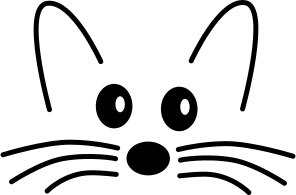
\includegraphics[width=1.4em]{squeak-logo}}}
\iftoshelse{
	\usepackage{marginnote}
		\renewcommand*{\marginfont}{\footnotesize}
	\newcommand{\vartriangleout}{\ifthenelse{\isodd{\thepage}}{\vartriangleright}{\vartriangleleft}}
	\newcommand{\dothisicon}{\fcolorbox{blue!65}{white}{\highlight{$\vartriangleout$}}}
	\newcommand{\dothis}[1]{%
		\noindent\par\noindent
		{\reversemarginpar
			\marginnote{\fcolorbox{blue!65}{white}{\highlight{$\vartriangleout$}}}}
		%\MarginLabel{do this}
		\noindent\emph{#1}
		\nopagebreak}
}{
	\newcommand{\dothisicon}{\raisebox{-.5ex}{
\includegraphics[height=1.2em]{pharo}}}
	\newcommand{\dothis}[1]{%
		\medskip
		\noindent\dothisicon
		\ifx#1\empty\else\quad\emph{#1}\fi
		\par\smallskip\nopagebreak}
}
%===> NEW VERSION <===
% NB: To use this in an individual chapter, you must set:
%\graphicspath{{figures/} {../figures/}}
% at the head of the chapter.  Don't forget the final /
%=============================================================
%:Reader hints (hint)
%
% Indicates a non-obvious consequence 
\newcommand{\hint}[1]{\vspace{1ex}\noindent\fbox{\textsc{Hint}} \emph{#1}}
%=================================================================
% graphics for Morphic handles
\newcommand{\grabHandle}{\raisebox{-0.2ex}{
\includegraphics[width=1em]{blackHandle}}}
\newcommand{\moveHandle}{\raisebox{-0.2ex}{
\includegraphics[width=1em]{moveHandle}}}
\newcommand{\debugHandle}{\raisebox{-0.2ex}{
\includegraphics[width=1em]{debugHandle}}}
%=============================================================
%:Highlighting Important stuff (doublebox)
%
% From Seaside book ...
\newsavebox{\SavedText}
\newlength{\InnerBoxRule}\setlength{\InnerBoxRule}{.75\fboxrule}
\newlength{\OuterBoxRule}\setlength{\OuterBoxRule}{1.5\fboxrule}
\newlength{\BoxSeparation}\setlength{\BoxSeparation}{1.5\fboxrule}
\addtolength{\BoxSeparation}{.5pt}
\newlength{\SaveBoxSep}\setlength{\SaveBoxSep}{2\fboxsep}
%
\newenvironment{doublebox}{\begin{lrbox}{\SavedText}
    \begin{minipage}{.75\textwidth}}
    {\end{minipage}\end{lrbox}\begin{center}
    \setlength{\fboxsep}{\BoxSeparation}\setlength{\fboxrule}{\OuterBoxRule}
    \fbox{\setlength{\fboxsep}{\SaveBoxSep}\setlength{\fboxrule}{\InnerBoxRule}%
      \fbox{\usebox{\SavedText}}}
  \end{center}}
% Use this:
\newcommand{\important}[1]{\begin{doublebox}#1\end{doublebox}}
%=============================================================
%:Section depth
\setcounter{secnumdepth}{2}
%% for this to happen start the file with
%\ifx\wholebook\relax\else
%% $Author$
% $Date$
% $Revision$

% HISTORY:
% 2006-10-31 - Oscar code macros
% ...

%=============================================================
% NB: documentclass must be set in main document.
% Allows book to be generated in multiple formats.
%=============================================================
%:Packages
\usepackage[T1]{fontenc}  %%%%%% really important to get the code directly in the text!
\usepackage{lmodern}
%\usepackage[scaled=0.85]{bookmanx} % needs another scale factor if used with \renewcommand{\sfdefault}{cmbr}
\usepackage{palatino}
\usepackage[scaled=0.85]{helvet}
\usepackage[protrusion,expansion=false]{microtype}
\usepackage{graphicx}
\usepackage{theorem}
\usepackage[english]{babel}
%%% ON: pdfsync breaks the use of p{width} for tabular columns!
%%\ifdefined\usepdfsync\usepackage{pdfsync}\fi % Requires texlive 2007
%=============================================================
%:More packages
%Stef should check which ones are used!
%\usepackage{picinpar}
%\usepackage{layout}
%\usepackage{color}
%\usepackage{enum}
%\usepackage{a4wide}
% \usepackage{fancyhdr}
\usepackage{ifthen}
\usepackage{float}
\usepackage{longtable}
\usepackage{makeidx}
\usepackage[nottoc]{tocbibind}
\usepackage{multicol}
\usepackage{booktabs}	% book-style tables
\usepackage{topcapt}	% enables \topcaption
\usepackage{multirow}
\usepackage{tabularx}
%\usepackage[bottom]{footmisc}
\usepackage{xspace}
\usepackage{alltt}
\usepackage{amssymb,textcomp}
\usepackage[usenames,dvipsnames]{color}
%\usepackage{colortbl}
\usepackage[hang]{subfigure}\makeatletter\def\p@subfigure{\thefigure\,}\makeatother
\usepackage{rotating}
\usepackage{enumitem}	% apb: allows more control over tags in enumerations
\usepackage{verbatim}     % for comment environment
\usepackage{varioref}	% for page references that work
\labelformat{footnote}{\thechapter--#1} % to distinguish citations from jurabib
\usepackage{needspace}
\usepackage{isodateo} % enable \isodate
\usepackage[newparttoc]{titlesec}
\usepackage{titletoc}
\usepackage{wrapfig}
\usepackage[
	super,
	citefull=first,
	authorformat={allreversed,and},
	titleformat={commasep,italic}
]{jurabib} % citations as footnotes
\usepackage[
	colorlinks=true,
	linkcolor=black,
	urlcolor=black,
	citecolor=black
]{hyperref}   % should come last
%=============================================================
%:PDF version
%%\pdfminorversion=3 % Set PDF to 1.3 for Lulu
%=============================================================
%:URL style
\makeatletter
\def\url@leostyle{%
  \@ifundefined{selectfont}{\def\UrlFont{\sf}}{\def\UrlFont{\sffamily}}}
\makeatother
% Now actually use the newly defined style.
\urlstyle{leo}
%=============================================================
%:Booleans
\newboolean{lulu}
\setboolean{lulu}{false}
\newcommand{\ifluluelse}[2]{\ifthenelse{\boolean{lulu}}{#1}{#2}}
%=============================================================
%:Names
\newcommand{\SUnit}{SUnit\xspace}
\newcommand{\sunit}{SUnit\xspace}
\newcommand{\xUnit}{$x$Unit\xspace}
\newcommand{\JUnit}{JUnit\xspace}
\newcommand{\st}{Smalltalk\xspace}
\newcommand{\pharo}{Pharo\xspace} % Use this, not \Pharo
%\newcommand{\sqmap}{SqueakMap\xspace}
\newcommand{\squeak}{Squeak\xspace} % use this, not \Squeak or \sq
\newcommand{\sqsrc}{SqueakSource\xspace}
\newcommand{\sbe}{\url{http://SqueakByExample.org}\xspace}
\newcommand{\pharoweb}{\url{http://pharo-project.org}\xspace}
\newcommand{\pbe}{\url{http://PharoByExample.org}\xspace}
\newcommand{\sba}{\url{http://SquareBracketAssociates.org}\xspace}
\newcommand{\bam}{\lct{Bounc\-ing\-Atoms\-Morph}\xspace}
%=============================================================
%:Markup macros for proof-reading
\usepackage[normalem]{ulem} % for \sout
\usepackage{xcolor}
\newcommand{\ra}{$\rightarrow$}
\newcommand{\ugh}[1]{\textcolor{red}{\uwave{#1}}} % please rephrase
\newcommand{\ins}[1]{\textcolor{blue}{\uline{#1}}} % please insert
\newcommand{\del}[1]{\textcolor{red}{\sout{#1}}} % please delete
\newcommand{\chg}[2]{\textcolor{red}{\sout{#1}}{\ra}\textcolor{blue}{\uline{#2}}} % please change
%=============================================================
%:Editorial comment macros
%\newcommand{\nnbb}[2]{
%    % \fbox{\bfseries\sffamily\scriptsize#1}
%    \fcolorbox{gray}{yellow}{\bfseries\sffamily\scriptsize#1}
%    {\sf\small$\blacktriangleright$\textit{#2}$\blacktriangleleft$}
%   }
\newcommand{\yellowbox}[1]{\fcolorbox{gray}{yellow}{\bfseries\sffamily\scriptsize#1}}
\newcommand{\triangles}[1]{{\sf\small$\blacktriangleright$\textit{#1}$\blacktriangleleft$}}
\newcommand{\nnbb}[2]{\yellowbox{#1} \triangles{#2}}
\newcommand{\fix}{\yellowbox{FIX!}}
\newcommand{\here}{\yellowbox{CONTINUE HERE!}}
% editor macros
\newcommand{\apl}[1]{\nnbb{Alain}{#1}} % Alain
\newcommand{\ab}[1]{\nnbb{Andrew}{#1}} % Black
\newcommand{\sd}[1]{\nnbb{St\'{e}f}{#1}} % Ducasse
\newcommand{\dc}[1]{\nnbb{DamienC}{#1}} % Ducasse
\newcommand{\md}[1]{\nnbb{Marcus}{#1}} % Denker
\newcommand{\on}[1]{\nnbb{Oscar}{#1}} % Nierstrasz
\newcommand{\damien}[1]{\nnbb{Damien}{#1}} % Pollet
\newcommand{\lr}[1]{\nnbb{Lukas}{#1}} % Renggli
\newcommand{\orla}[1]{\nnbb{Orla}{#1}} % Greevy
\newcommand{\alex}[1]{\nnbb{Alex}{#1}} % Bergel
\newcommand{\alx}[1]{\nnbb{Alex}{#1}} % Bergel
\newcommand{\dr}[1]{\nnbb{David}{#1}} % Roethlisberger
\newcommand{\ja}[1]{\nnbb{Jannik}{#1}} % Laval
\newcommand{\jr}[1]{\nnbb{Jorge}{#1}} % Ressia
\newcommand{\fp}[1]{\nnbb{Fabrizio}{#1}} % Perin
\newcommand{\michael}[1]{\nnbb{Michael}{#1}} % Davies
\newcommand{\ew}[1]{\nnbb{Erwann}{#1}} % Wernli
\newcommand{\mb}[1]{\nnbb{Martial}{#1}} % Boniou
\newcommand{\hw}[1]{\nnbb{Hernan}{#1}} % Wilkinson
%=============================================================
%:Abbreviation macros
\newcommand{\ie}{\emph{すなわち}、}
\newcommand{\eg}{\emph{例えば}、}
\newcommand{\etc}{などなど。}
%=============================================================
%:Cross reference macros
\newcommand{\charef}[1]{第~\ref{cha:#1}~章}
\newcommand{\secref}[1]{\ref{sec:#1}~節}
\newcommand{\figref}[1]{図~\ref{fig:#1}\xspace}
\newcommand{\Figref}[1]{図~\ref{fig:#1}\xspace}
\newcommand{\appref}[1]{付録~\ref{app:#1}\xspace}
\newcommand{\tabref}[1]{表~\ref{tab:#1}\xspace}
\newcommand{\faqref}[1]{FAQ~\ref{faq:#1}, p.~\pageref{faq:#1}\xspace}
% APB: I removed trailing \xspace commands from these macros because
% \xspace mostly doesn't work.  If you want a space after your
% references, type one!
% ON: xspace has always worked just fine for me!  Please leave them in.
%
\newcommand{\ruleref}[1]{\ref{rule:#1}\xspace}
%
\newcommand{\egref}[1]{example~\ref{eg:#1}\xspace}
\newcommand{\Egref}[1]{Example~\ref{eg:#1}\xspace}
%
\newcommand{\scrref}[1]{script~\ref{scr:#1}\xspace}
\newcommand{\Scrref}[1]{Script~\ref{scr:#1}\xspace}
\newcommand{\tscrref}[1]{the script~\ref{scr:#1}\xspace}
\newcommand{\Tscrref}[1]{The script~\ref{scr:#1}\xspace}
%
\newcommand{\mthref}[1]{method~\ref{mth:#1}\xspace}
\newcommand{\mthsref}[1]{methods~\ref{mth:#1}\xspace}
\newcommand{\Mthref}[1]{Method~\ref{mth:#1}\xspace}
\newcommand{\tmthref}[1]{the method~\ref{mth:#1}\xspace}
\newcommand{\Tmthref}[1]{The method~\ref{mth:#1}\xspace}
%
\newcommand{\clsref}[1]{class~\ref{cls:#1}\xspace}
\newcommand{\tclsref}[1]{the class~\ref{cls:#1}\xspace}
\newcommand{\Tclsref}[1]{The class~\ref{cls:#1}\xspace}

\newcommand{\chalabel}[1]{\label{cha:#1}}
\newcommand{\seclabel}[1]{\label{sec:#1}}
\newcommand{\figlabel}[1]{\label{fig:#1}}
\newcommand{\tablabel}[1]{\label{tab:#1}}
\newcommand{\rulelabel}[1]{\label{rule:#1}}
\newcommand{\eglabel}[1]{\label{eg:#1}}
\newcommand{\scrlabel}[1]{\label{scr:#1}}
\newcommand{\mthlabel}[1]{\label{mth:#1}}
\newcommand{\clslabel}[1]{\label{cls:#1}}
\newcommand{\faqlabel}[1]{\label{faq:#1}}
%=============================================================
%:Menu item macro
% for menu items, so we can change our minds on how to print them! (apb)
\definecolor{lightgray}{gray}{0.89}
\newcommand{\menu}[1]{{%
	\setlength{\fboxsep}{0pt}%
	\colorbox{lightgray}{{{\upshape\sffamily\strut \,#1\,}}}}}
\newcommand{\link}[1]{{%
	\fontfamily{lmr}\selectfont
 	\upshape{\sffamily \underline{#1}}}}
% For submenu items:
\newcommand{\go}{\,$\triangleright$\,}
% \newcommand{\go}{\,$\blacktriangleright$\,}
% For keyboard shortcuts:
%\newcommand{\short}[1]{\mbox{$\langle${\sc CMD}$\rangle$-#1}\xspace}
\newcommand{\short}[1]{\mbox{{\sc cmd}\hspace{0.08em}--\hspace{0.09em}#1}\xspace}
% For buttons:
\newcommand{\button}[1]{{%
	\setlength{\fboxsep}{0pt}%
	\fbox{{\upshape\sffamily\strut \,#1\,}}}}
% NB: The button macro does not work within captions -- incompatible with xcolor package :-(
\newcommand{\toolsflap}{\textit{Tools} flap\xspace}
%=============================================================
%:Mouse clicks
\newcommand{\click}{click\xspace} % RED
\newcommand{\actclick}{action-click\xspace} % YELLOW
\newcommand{\metaclick}{meta-click\xspace} % BLUE
\newcommand{\Click}{Click\xspace} % RED
\newcommand{\Actclick}{Action-click\xspace} % YELLOW
\newcommand{\Metaclick}{Meta-click\xspace} % BLUE
%=============================================================
%:ToSh macros
\newboolean{tosh}
\setboolean{tosh}{false}
\newcommand{\iftoshelse}[2]{\ifthenelse{\boolean{tosh}}{#1}{#2}}
%=============================================================
%:ToSh colors
%\newcommand{\highlightcolor}{\color{blue!65}}
%\newcommand{\boxcolor}{\color{gray!25}}
\newcommand{\highlight}[1]{\textcolor{blue!65}{#1}}
%\newcommand{\codecolor}{\color{blue!65}}
%%\setlength{\fboxrule}{2pt}
%\newcommand{\asPict}[1]{%
%	{\Large\highlight{#1}}}
%=============================================================
%:Reader cues (do this)
%
% Indicate something the reader should try out.
% \newcommand{\dothisicon}{\raisebox{-.5ex}{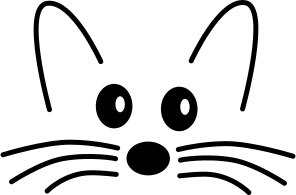
\includegraphics[width=1.4em]{squeak-logo}}}
\iftoshelse{
	\usepackage{marginnote}
		\renewcommand*{\marginfont}{\footnotesize}
	\newcommand{\vartriangleout}{\ifthenelse{\isodd{\thepage}}{\vartriangleright}{\vartriangleleft}}
	\newcommand{\dothisicon}{\fcolorbox{blue!65}{white}{\highlight{$\vartriangleout$}}}
	\newcommand{\dothis}[1]{%
		\noindent\par\noindent
		{\reversemarginpar
			\marginnote{\fcolorbox{blue!65}{white}{\highlight{$\vartriangleout$}}}}
		%\MarginLabel{do this}
		\noindent\emph{#1}
		\nopagebreak}
}{
	\newcommand{\dothisicon}{\raisebox{-.5ex}{
\includegraphics[height=1.2em]{pharo}}}
	\newcommand{\dothis}[1]{%
		\medskip
		\noindent\dothisicon
		\ifx#1\empty\else\quad\emph{#1}\fi
		\par\smallskip\nopagebreak}
}
%===> NEW VERSION <===
% NB: To use this in an individual chapter, you must set:
%\graphicspath{{figures/} {../figures/}}
% at the head of the chapter.  Don't forget the final /
%=============================================================
%:Reader hints (hint)
%
% Indicates a non-obvious consequence 
\newcommand{\hint}[1]{\vspace{1ex}\noindent\fbox{\textsc{Hint}} \emph{#1}}
%=================================================================
% graphics for Morphic handles
\newcommand{\grabHandle}{\raisebox{-0.2ex}{
\includegraphics[width=1em]{blackHandle}}}
\newcommand{\moveHandle}{\raisebox{-0.2ex}{
\includegraphics[width=1em]{moveHandle}}}
\newcommand{\debugHandle}{\raisebox{-0.2ex}{
\includegraphics[width=1em]{debugHandle}}}
%=============================================================
%:Highlighting Important stuff (doublebox)
%
% From Seaside book ...
\newsavebox{\SavedText}
\newlength{\InnerBoxRule}\setlength{\InnerBoxRule}{.75\fboxrule}
\newlength{\OuterBoxRule}\setlength{\OuterBoxRule}{1.5\fboxrule}
\newlength{\BoxSeparation}\setlength{\BoxSeparation}{1.5\fboxrule}
\addtolength{\BoxSeparation}{.5pt}
\newlength{\SaveBoxSep}\setlength{\SaveBoxSep}{2\fboxsep}
%
\newenvironment{doublebox}{\begin{lrbox}{\SavedText}
    \begin{minipage}{.75\textwidth}}
    {\end{minipage}\end{lrbox}\begin{center}
    \setlength{\fboxsep}{\BoxSeparation}\setlength{\fboxrule}{\OuterBoxRule}
    \fbox{\setlength{\fboxsep}{\SaveBoxSep}\setlength{\fboxrule}{\InnerBoxRule}%
      \fbox{\usebox{\SavedText}}}
  \end{center}}
% Use this:
\newcommand{\important}[1]{\begin{doublebox}#1\end{doublebox}}
%=============================================================
%:Section depth
\setcounter{secnumdepth}{2}
%% for this to happen start the file with
%\ifx\wholebook\relax\else
%% $Author$
% $Date$
% $Revision$

% HISTORY:
% 2006-10-31 - Oscar code macros
% ...

%=============================================================
% NB: documentclass must be set in main document.
% Allows book to be generated in multiple formats.
%=============================================================
%:Packages
\usepackage[T1]{fontenc}  %%%%%% really important to get the code directly in the text!
\usepackage{lmodern}
%\usepackage[scaled=0.85]{bookmanx} % needs another scale factor if used with \renewcommand{\sfdefault}{cmbr}
\usepackage{palatino}
\usepackage[scaled=0.85]{helvet}
\usepackage[protrusion,expansion=false]{microtype}
\usepackage{graphicx}
\usepackage{theorem}
\usepackage[english]{babel}
%%% ON: pdfsync breaks the use of p{width} for tabular columns!
%%\ifdefined\usepdfsync\usepackage{pdfsync}\fi % Requires texlive 2007
%=============================================================
%:More packages
%Stef should check which ones are used!
%\usepackage{picinpar}
%\usepackage{layout}
%\usepackage{color}
%\usepackage{enum}
%\usepackage{a4wide}
% \usepackage{fancyhdr}
\usepackage{ifthen}
\usepackage{float}
\usepackage{longtable}
\usepackage{makeidx}
\usepackage[nottoc]{tocbibind}
\usepackage{multicol}
\usepackage{booktabs}	% book-style tables
\usepackage{topcapt}	% enables \topcaption
\usepackage{multirow}
\usepackage{tabularx}
%\usepackage[bottom]{footmisc}
\usepackage{xspace}
\usepackage{alltt}
\usepackage{amssymb,textcomp}
\usepackage[usenames,dvipsnames]{color}
%\usepackage{colortbl}
\usepackage[hang]{subfigure}\makeatletter\def\p@subfigure{\thefigure\,}\makeatother
\usepackage{rotating}
\usepackage{enumitem}	% apb: allows more control over tags in enumerations
\usepackage{verbatim}     % for comment environment
\usepackage{varioref}	% for page references that work
\labelformat{footnote}{\thechapter--#1} % to distinguish citations from jurabib
\usepackage{needspace}
\usepackage{isodateo} % enable \isodate
\usepackage[newparttoc]{titlesec}
\usepackage{titletoc}
\usepackage{wrapfig}
\usepackage[
	super,
	citefull=first,
	authorformat={allreversed,and},
	titleformat={commasep,italic}
]{jurabib} % citations as footnotes
\usepackage[
	colorlinks=true,
	linkcolor=black,
	urlcolor=black,
	citecolor=black
]{hyperref}   % should come last
%=============================================================
%:PDF version
%%\pdfminorversion=3 % Set PDF to 1.3 for Lulu
%=============================================================
%:URL style
\makeatletter
\def\url@leostyle{%
  \@ifundefined{selectfont}{\def\UrlFont{\sf}}{\def\UrlFont{\sffamily}}}
\makeatother
% Now actually use the newly defined style.
\urlstyle{leo}
%=============================================================
%:Booleans
\newboolean{lulu}
\setboolean{lulu}{false}
\newcommand{\ifluluelse}[2]{\ifthenelse{\boolean{lulu}}{#1}{#2}}
%=============================================================
%:Names
\newcommand{\SUnit}{SUnit\xspace}
\newcommand{\sunit}{SUnit\xspace}
\newcommand{\xUnit}{$x$Unit\xspace}
\newcommand{\JUnit}{JUnit\xspace}
\newcommand{\st}{Smalltalk\xspace}
\newcommand{\pharo}{Pharo\xspace} % Use this, not \Pharo
%\newcommand{\sqmap}{SqueakMap\xspace}
\newcommand{\squeak}{Squeak\xspace} % use this, not \Squeak or \sq
\newcommand{\sqsrc}{SqueakSource\xspace}
\newcommand{\sbe}{\url{http://SqueakByExample.org}\xspace}
\newcommand{\pharoweb}{\url{http://pharo-project.org}\xspace}
\newcommand{\pbe}{\url{http://PharoByExample.org}\xspace}
\newcommand{\sba}{\url{http://SquareBracketAssociates.org}\xspace}
\newcommand{\bam}{\lct{Bounc\-ing\-Atoms\-Morph}\xspace}
%=============================================================
%:Markup macros for proof-reading
\usepackage[normalem]{ulem} % for \sout
\usepackage{xcolor}
\newcommand{\ra}{$\rightarrow$}
\newcommand{\ugh}[1]{\textcolor{red}{\uwave{#1}}} % please rephrase
\newcommand{\ins}[1]{\textcolor{blue}{\uline{#1}}} % please insert
\newcommand{\del}[1]{\textcolor{red}{\sout{#1}}} % please delete
\newcommand{\chg}[2]{\textcolor{red}{\sout{#1}}{\ra}\textcolor{blue}{\uline{#2}}} % please change
%=============================================================
%:Editorial comment macros
%\newcommand{\nnbb}[2]{
%    % \fbox{\bfseries\sffamily\scriptsize#1}
%    \fcolorbox{gray}{yellow}{\bfseries\sffamily\scriptsize#1}
%    {\sf\small$\blacktriangleright$\textit{#2}$\blacktriangleleft$}
%   }
\newcommand{\yellowbox}[1]{\fcolorbox{gray}{yellow}{\bfseries\sffamily\scriptsize#1}}
\newcommand{\triangles}[1]{{\sf\small$\blacktriangleright$\textit{#1}$\blacktriangleleft$}}
\newcommand{\nnbb}[2]{\yellowbox{#1} \triangles{#2}}
\newcommand{\fix}{\yellowbox{FIX!}}
\newcommand{\here}{\yellowbox{CONTINUE HERE!}}
% editor macros
\newcommand{\apl}[1]{\nnbb{Alain}{#1}} % Alain
\newcommand{\ab}[1]{\nnbb{Andrew}{#1}} % Black
\newcommand{\sd}[1]{\nnbb{St\'{e}f}{#1}} % Ducasse
\newcommand{\dc}[1]{\nnbb{DamienC}{#1}} % Ducasse
\newcommand{\md}[1]{\nnbb{Marcus}{#1}} % Denker
\newcommand{\on}[1]{\nnbb{Oscar}{#1}} % Nierstrasz
\newcommand{\damien}[1]{\nnbb{Damien}{#1}} % Pollet
\newcommand{\lr}[1]{\nnbb{Lukas}{#1}} % Renggli
\newcommand{\orla}[1]{\nnbb{Orla}{#1}} % Greevy
\newcommand{\alex}[1]{\nnbb{Alex}{#1}} % Bergel
\newcommand{\alx}[1]{\nnbb{Alex}{#1}} % Bergel
\newcommand{\dr}[1]{\nnbb{David}{#1}} % Roethlisberger
\newcommand{\ja}[1]{\nnbb{Jannik}{#1}} % Laval
\newcommand{\jr}[1]{\nnbb{Jorge}{#1}} % Ressia
\newcommand{\fp}[1]{\nnbb{Fabrizio}{#1}} % Perin
\newcommand{\michael}[1]{\nnbb{Michael}{#1}} % Davies
\newcommand{\ew}[1]{\nnbb{Erwann}{#1}} % Wernli
\newcommand{\mb}[1]{\nnbb{Martial}{#1}} % Boniou
\newcommand{\hw}[1]{\nnbb{Hernan}{#1}} % Wilkinson
%=============================================================
%:Abbreviation macros
\newcommand{\ie}{\emph{すなわち}、}
\newcommand{\eg}{\emph{例えば}、}
\newcommand{\etc}{などなど。}
%=============================================================
%:Cross reference macros
\newcommand{\charef}[1]{第~\ref{cha:#1}~章}
\newcommand{\secref}[1]{\ref{sec:#1}~節}
\newcommand{\figref}[1]{図~\ref{fig:#1}\xspace}
\newcommand{\Figref}[1]{図~\ref{fig:#1}\xspace}
\newcommand{\appref}[1]{付録~\ref{app:#1}\xspace}
\newcommand{\tabref}[1]{表~\ref{tab:#1}\xspace}
\newcommand{\faqref}[1]{FAQ~\ref{faq:#1}, p.~\pageref{faq:#1}\xspace}
% APB: I removed trailing \xspace commands from these macros because
% \xspace mostly doesn't work.  If you want a space after your
% references, type one!
% ON: xspace has always worked just fine for me!  Please leave them in.
%
\newcommand{\ruleref}[1]{\ref{rule:#1}\xspace}
%
\newcommand{\egref}[1]{example~\ref{eg:#1}\xspace}
\newcommand{\Egref}[1]{Example~\ref{eg:#1}\xspace}
%
\newcommand{\scrref}[1]{script~\ref{scr:#1}\xspace}
\newcommand{\Scrref}[1]{Script~\ref{scr:#1}\xspace}
\newcommand{\tscrref}[1]{the script~\ref{scr:#1}\xspace}
\newcommand{\Tscrref}[1]{The script~\ref{scr:#1}\xspace}
%
\newcommand{\mthref}[1]{method~\ref{mth:#1}\xspace}
\newcommand{\mthsref}[1]{methods~\ref{mth:#1}\xspace}
\newcommand{\Mthref}[1]{Method~\ref{mth:#1}\xspace}
\newcommand{\tmthref}[1]{the method~\ref{mth:#1}\xspace}
\newcommand{\Tmthref}[1]{The method~\ref{mth:#1}\xspace}
%
\newcommand{\clsref}[1]{class~\ref{cls:#1}\xspace}
\newcommand{\tclsref}[1]{the class~\ref{cls:#1}\xspace}
\newcommand{\Tclsref}[1]{The class~\ref{cls:#1}\xspace}

\newcommand{\chalabel}[1]{\label{cha:#1}}
\newcommand{\seclabel}[1]{\label{sec:#1}}
\newcommand{\figlabel}[1]{\label{fig:#1}}
\newcommand{\tablabel}[1]{\label{tab:#1}}
\newcommand{\rulelabel}[1]{\label{rule:#1}}
\newcommand{\eglabel}[1]{\label{eg:#1}}
\newcommand{\scrlabel}[1]{\label{scr:#1}}
\newcommand{\mthlabel}[1]{\label{mth:#1}}
\newcommand{\clslabel}[1]{\label{cls:#1}}
\newcommand{\faqlabel}[1]{\label{faq:#1}}
%=============================================================
%:Menu item macro
% for menu items, so we can change our minds on how to print them! (apb)
\definecolor{lightgray}{gray}{0.89}
\newcommand{\menu}[1]{{%
	\setlength{\fboxsep}{0pt}%
	\colorbox{lightgray}{{{\upshape\sffamily\strut \,#1\,}}}}}
\newcommand{\link}[1]{{%
	\fontfamily{lmr}\selectfont
 	\upshape{\sffamily \underline{#1}}}}
% For submenu items:
\newcommand{\go}{\,$\triangleright$\,}
% \newcommand{\go}{\,$\blacktriangleright$\,}
% For keyboard shortcuts:
%\newcommand{\short}[1]{\mbox{$\langle${\sc CMD}$\rangle$-#1}\xspace}
\newcommand{\short}[1]{\mbox{{\sc cmd}\hspace{0.08em}--\hspace{0.09em}#1}\xspace}
% For buttons:
\newcommand{\button}[1]{{%
	\setlength{\fboxsep}{0pt}%
	\fbox{{\upshape\sffamily\strut \,#1\,}}}}
% NB: The button macro does not work within captions -- incompatible with xcolor package :-(
\newcommand{\toolsflap}{\textit{Tools} flap\xspace}
%=============================================================
%:Mouse clicks
\newcommand{\click}{click\xspace} % RED
\newcommand{\actclick}{action-click\xspace} % YELLOW
\newcommand{\metaclick}{meta-click\xspace} % BLUE
\newcommand{\Click}{Click\xspace} % RED
\newcommand{\Actclick}{Action-click\xspace} % YELLOW
\newcommand{\Metaclick}{Meta-click\xspace} % BLUE
%=============================================================
%:ToSh macros
\newboolean{tosh}
\setboolean{tosh}{false}
\newcommand{\iftoshelse}[2]{\ifthenelse{\boolean{tosh}}{#1}{#2}}
%=============================================================
%:ToSh colors
%\newcommand{\highlightcolor}{\color{blue!65}}
%\newcommand{\boxcolor}{\color{gray!25}}
\newcommand{\highlight}[1]{\textcolor{blue!65}{#1}}
%\newcommand{\codecolor}{\color{blue!65}}
%%\setlength{\fboxrule}{2pt}
%\newcommand{\asPict}[1]{%
%	{\Large\highlight{#1}}}
%=============================================================
%:Reader cues (do this)
%
% Indicate something the reader should try out.
% \newcommand{\dothisicon}{\raisebox{-.5ex}{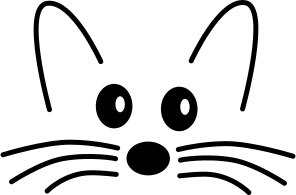
\includegraphics[width=1.4em]{squeak-logo}}}
\iftoshelse{
	\usepackage{marginnote}
		\renewcommand*{\marginfont}{\footnotesize}
	\newcommand{\vartriangleout}{\ifthenelse{\isodd{\thepage}}{\vartriangleright}{\vartriangleleft}}
	\newcommand{\dothisicon}{\fcolorbox{blue!65}{white}{\highlight{$\vartriangleout$}}}
	\newcommand{\dothis}[1]{%
		\noindent\par\noindent
		{\reversemarginpar
			\marginnote{\fcolorbox{blue!65}{white}{\highlight{$\vartriangleout$}}}}
		%\MarginLabel{do this}
		\noindent\emph{#1}
		\nopagebreak}
}{
	\newcommand{\dothisicon}{\raisebox{-.5ex}{
\includegraphics[height=1.2em]{pharo}}}
	\newcommand{\dothis}[1]{%
		\medskip
		\noindent\dothisicon
		\ifx#1\empty\else\quad\emph{#1}\fi
		\par\smallskip\nopagebreak}
}
%===> NEW VERSION <===
% NB: To use this in an individual chapter, you must set:
%\graphicspath{{figures/} {../figures/}}
% at the head of the chapter.  Don't forget the final /
%=============================================================
%:Reader hints (hint)
%
% Indicates a non-obvious consequence 
\newcommand{\hint}[1]{\vspace{1ex}\noindent\fbox{\textsc{Hint}} \emph{#1}}
%=================================================================
% graphics for Morphic handles
\newcommand{\grabHandle}{\raisebox{-0.2ex}{
\includegraphics[width=1em]{blackHandle}}}
\newcommand{\moveHandle}{\raisebox{-0.2ex}{
\includegraphics[width=1em]{moveHandle}}}
\newcommand{\debugHandle}{\raisebox{-0.2ex}{
\includegraphics[width=1em]{debugHandle}}}
%=============================================================
%:Highlighting Important stuff (doublebox)
%
% From Seaside book ...
\newsavebox{\SavedText}
\newlength{\InnerBoxRule}\setlength{\InnerBoxRule}{.75\fboxrule}
\newlength{\OuterBoxRule}\setlength{\OuterBoxRule}{1.5\fboxrule}
\newlength{\BoxSeparation}\setlength{\BoxSeparation}{1.5\fboxrule}
\addtolength{\BoxSeparation}{.5pt}
\newlength{\SaveBoxSep}\setlength{\SaveBoxSep}{2\fboxsep}
%
\newenvironment{doublebox}{\begin{lrbox}{\SavedText}
    \begin{minipage}{.75\textwidth}}
    {\end{minipage}\end{lrbox}\begin{center}
    \setlength{\fboxsep}{\BoxSeparation}\setlength{\fboxrule}{\OuterBoxRule}
    \fbox{\setlength{\fboxsep}{\SaveBoxSep}\setlength{\fboxrule}{\InnerBoxRule}%
      \fbox{\usebox{\SavedText}}}
  \end{center}}
% Use this:
\newcommand{\important}[1]{\begin{doublebox}#1\end{doublebox}}
%=============================================================
%:Section depth
\setcounter{secnumdepth}{2}
%% for this to happen start the file with
%\ifx\wholebook\relax\else
%\input{../common.tex}
%\begin{document}
%\fi
% and terminate by
% \ifx\wholebook\relax\else\end{document}\fi

\DeclareGraphicsExtensions{.pdf, .jpg, .png}
%=============================================================
%:PDF setup
\hypersetup{
%   a4paper,
%   pdfstartview=FitV,
%   colorlinks,
%   linkcolor=darkblue,
%   citecolor=darkblue,
   pdftitle={Pharo by Example},
   pdfauthor={Andrew P. Black, St\'ephane Ducasse,	Oscar Nierstrasz,
Damien Pollet},
   pdfkeywords={Smalltalk, Squeak, Object-Oriented Programming, OOP},
   pdfsubject={Computer Science}
}
%=============================================================
%:Page layout and appearance
%
% \renewcommand{\headrulewidth}{0pt}
\renewcommand{\chaptermark}[1]{\markboth{#1}{}}
\renewcommand{\sectionmark}[1]{\markright{\thesection\ #1}}
\renewpagestyle{plain}[\small\itshape]{%
	\setheadrule{0pt}%
	\sethead[][][]{}{}{}%
	\setfoot[][][]{}{}{}}
\renewpagestyle{headings}[\small\itshape]{%
	\setheadrule{0pt}%
	\setmarks{chapter}{section}%
	\sethead[\thepage][][\chaptertitle]{\sectiontitle}{}{\thepage}%
	\setfoot[][][]{}{}{}}
%=============================================================
%:Title section setup and TOC numbering depth
\setcounter{secnumdepth}{1}
\setcounter{tocdepth}{1}
\titleformat{\part}[display]{\centering}{\huge\partname\ \thepart}{1em}{\Huge\textbf}[]
\titleformat{\chapter}[display]{}{\huge\chaptertitlename\ \thechapter}{1em}{\Huge\raggedright\textbf}[]
\titlecontents{part}[3pc]{%
		\pagebreak[2]\addvspace{1em plus.4em minus.2em}%
		\leavevmode\large\bfseries}
	{\contentslabel{3pc}}{\hspace*{-3pc}}
	{}[\nopagebreak]
\titlecontents{chapter}[3pc]{%
		\pagebreak[0]\addvspace{1em plus.2em minus.2em}%
		\leavevmode\bfseries}
	{\contentslabel{3pc}}{}
	{\hfill\contentspage}[\nopagebreak]
\dottedcontents{section}[3pc]{}{3pc}{1pc}
\dottedcontents{subsection}[3pc]{}{0pc}{1pc}
% \dottedcontents{subsection}[4.5em]{}{0pt}{1pc}
% Make \cleardoublepage insert really blank pages http://www.tex.ac.uk/cgi-bin/texfaq2html?label=reallyblank
\let\origdoublepage\cleardoublepage
\newcommand{\clearemptydoublepage}{%
  \clearpage
  {\pagestyle{empty}\origdoublepage}}
\let\cleardoublepage\clearemptydoublepage % see http://www.tex.ac.uk/cgi-bin/texfaq2html?label=patch
%=============================================================
%:FAQ macros (for FAQ chapter)
\newtheorem{faq}{FAQ}
\newcommand{\answer}{\paragraph{Answer}\ }
%=============================================================
%:Listings package configuration
% \newcommand{\caret}{\makebox{\raisebox{0.4ex}{\footnotesize{$\wedge$}}}}
\newcommand{\caret}{\^\,}
\newcommand{\escape}{{\sf \textbackslash}}
\definecolor{source}{gray}{0.95}
\usepackage{listings}
\lstdefinelanguage{Smalltalk}{
%  morekeywords={self,super,true,false,nil,thisContext}, % This is overkill
  morestring=[d]',
  morecomment=[s]{"}{"},
  alsoletter={\#:},
  escapechar={!},
  literate=
    {BANG}{!}1
    {CARET}{\^}1
    {UNDERSCORE}{\_}1
    {\\st}{Smalltalk}9 % convenience -- in case \st occurs in code
    % {'}{{\textquotesingle}}1 % replaced by upquote=true in \lstset
    {_}{{$\leftarrow$}}1
    {>>>}{{\sep}}1
    {^}{{$\uparrow$}}1
    {~}{{$\sim$}}1
    {-}{{\texttt{-}}}1 %{\textminus}}1 %{-}{\hspace{-0.13em}}{-}}1  % the goal is to make - the same width as +
    % {+}{\sf+}1 %{\raisebox{0.08ex}{+}}}1      % and to raise + off the baseline to match -
    {-->}{{\quad$\longrightarrow$\quad}}3
	, % Don't forget the comma at the end!
  tabsize=4
}[keywords,comments,strings]

\lstset{language=Smalltalk,
	basicstyle=\sffamily,
	keywordstyle=\color{black}\bfseries,
	% stringstyle=\ttfamily, % Ugly! do we really want this? -- on
	mathescape=true,
	showstringspaces=false,
	keepspaces=true,
	breaklines=true,
	breakautoindent=true,
	backgroundcolor=\color{source},
	lineskip={-1pt}, % Ugly hack
	upquote=true, % straight quote; requires textcomp package
	columns=fullflexible} % no fixed width fonts
% In-line code (literal)
% Normally use this for all in-line code:
\newcommand{\ct}{\lstinline[mathescape=false,backgroundcolor=\color{white},basicstyle={\sffamily\upshape}]}
% apb 2007.8.28 added the \upshape declaration to avoid getting italicized code in \dothis{ } sections.
% In-line code (latex enabled)
% Use this only in special situations where \ct does not work
% (within section headings ...):
\newcommand{\lct}[1]{{\textsf{\textup{#1}}}}
% Use these for system categories and protocols:
\newcommand{\scat}[1]{\emph{\textsf{#1}}\xspace}
\newcommand{\pkg}[1]{\emph{\textsf{#1}}\xspace}
\newcommand{\prot}[1]{\emph{\textsf{#1}}\xspace}
% Code environments
% NB: the arg is for tests
% Only code and example environments may be tests
\lstnewenvironment{code}[1]{%
	\lstset{%
		% frame=lines,
		frame=single,
		framerule=0pt,
		mathescape=false
	}
}{}
\def\ignoredollar#1{}
%=============================================================
%:Code environments (method, script ...)
% NB: the third arg is for tests
% Only code and example environments may be tests
\lstnewenvironment{example}[3][defaultlabel]{%
	\renewcommand{\lstlistingname}{Example}%
	\lstset{
		% frame=lines,
		frame=single,
		framerule=0pt,
		mathescape=false,
		caption={\emph{#2}},
		label={eg:#1}
	}
}{}
\lstnewenvironment{script}[2][defaultlabel]{%
\renewcommand{\lstlistingname}{Script}%
	\lstset{
		% frame=lines,
		frame=single,
		framerule=0pt,
		mathescape=false,
		name={Script},
		caption={\emph{#2}},
		label={scr:#1}
	}
}{}
\lstnewenvironment{method}[2][defaultlabel]{%
	\renewcommand{\lstlistingname}{Method}%
	\lstset{
		% frame=lines,
		frame=single,
		framerule=0pt,
		mathescape=false,
		name={Method},
		caption={\emph{#2}},
		label={mth:#1}
	}
}{}
\lstnewenvironment{methods}[2][defaultlabel]{% just for multiple methods at once
	\renewcommand{\lstlistingname}{Methods}%
	\lstset{
		% frame=lines,
		frame=single,
		framerule=0pt,
		mathescape=false,
		name={Method},
		caption={\emph{#2}},
		label={mth:#1}
	}
}{}
\lstnewenvironment{numMethod}[2][defaultlabel]{%
	\renewcommand{\lstlistingname}{Method}%
	\lstset{
		numbers=left,
		numberstyle={\tiny\sffamily},
		% frame=lines,
		frame=single,
		framerule=0pt,
		mathescape=false,
		name={Method},
		caption={\emph{#2}},
		label={mth:#1}
	}
}{}
\lstnewenvironment{classdef}[2][defaultlabel]{%
	\renewcommand{\lstlistingname}{Class}%
	\lstset{
		% frame=lines,
		frame=single,
		framerule=0pt,
		mathescape=false,
		name={Class},
		caption={\emph{#2}},
		label={cls:#1}
	}
}{}
%=============================================================
%:Reserving space
% Usually need one more line than the actual lines of code
\newcommand{\needlines}[1]{\Needspace{#1\baselineskip}}
%=============================================================
%:Indexing macros
% Macros ending with "ind" generate text as well as an index entry
% Macros ending with "index" *only* generate an index entry
\newcommand{\ind}[1]{\index{#1}#1\xspace} % plain text
\newcommand{\subind}[2]{\index{#1!#2}#2\xspace} % show #2, subindex under #1
\newcommand{\emphind}[1]{\index{#1}\emph{#1}\xspace} % emph #1
\newcommand{\emphsubind}[2]{\index{#1!#2}\emph{#2}\xspace} % show emph #2, subindex inder #1
\newcommand{\scatind}[1]{\index{#1@\textsf{#1} (category)}\scat{#1}} % category
\newcommand{\pkgind}[1]{\index{#1@\textsf{#1} (package)}\pkg{#1}} % package
\newcommand{\protind}[1]{\index{#1@\textsf{#1} (protocol)}\prot{#1}} % protocol
\newcommand{\clsind}[1]{\index{#1@\textsf{#1} (class)}\ct{#1}\xspace}
% \newcommand{\clsind}[1]{\index{#1!\#@(class)}\ct{#1}\xspace} % class
\newcommand{\clsindplural}[1]{\index{#1!\#@(class)}\ct{#1}s\xspace} % class
\newcommand{\cvind}[1]{\index{#1@\textsf{#1} (class variable)}\ct{#1}\xspace} % class var
\newcommand{\glbind}[1]{\index{#1@\textsf{#1} (global)}\ct{#1}\xspace} % global
\newcommand{\patind}[1]{\index{#1@#1 (pattern)}\ct{#1}\xspace} % pattern
\newcommand{\pvind}[1]{\index{#1@\textsf{#1} (pseudo variable)}\ct{#1}\xspace} % pseudo var
\newcommand{\clsmthind}[2]{\index{#1!#2@\ct{#2}}\ct{#1>>>#2}\xspace} % class + method name
\newcommand{\mthind}[2]{\index{#1!#2@\ct{#2}}\ct{#2}\xspace} % show method name only
\newcommand{\lmthind}[2]{\index{#1!#2@\ct{#2}}\lct{#2}\xspace} % show method name only
\newcommand{\cmind}[2]{\index{#1!#2@\ct{#2}}\ct{#1>>>#2}\xspace} % show class>>method
\newcommand{\lcmind}[2]{\index{#1!#2@\ct{#2}}\lct{#1>>>#2}\xspace} % show class>>method
\newcommand{\toolsflapind}{\index{Tools flap}\toolsflap} % index tools flap
% The following only generate an index entry:
% \newcommand{\clsindex}[1]{\index{#1@\textsf{#1} (class)}}
\newcommand{\clsindex}[1]{\index{#1!\#@(class)}} % class
\newcommand{\mthindex}[2]{\index{#1!#2@\ct{#2}}} % method
\newcommand{\cmindex}[2]{\index{#1!#2@\ct{#2}}} % class>>method
\newcommand{\cvindex}[1]{\index{#1@\textsf{#1} (class variable)}} % class var
\newcommand{\glbindex}[1]{\index{#1@\textsf{#1} (global)}}% global
\newcommand{\pvindex}[1]{\index{#1@\textsf{#1} (pseudo variable)}}% pseudo var
\newcommand{\seeindex}[2]{\index{#1|see{#2}}} % #1, see #2
\newcommand{\scatindex}[1]{\index{#1@\textsf{#1} (category)}} % category
\newcommand{\pkgindex}[1]{\index{#1@\textsf{#1} (package)}} % package
\newcommand{\protindex}[1]{\index{#1@\textsf{#1} (protocol)}} % protocol
% How can we have the main entry page numbers in bold yet not break the hyperlink?
\newcommand{\boldidx}[1]{{\bf #1}} % breaks hyperlink
%\newcommand{\indmain}[1]{\index{#1|boldidx}#1\xspace} % plain text, main entry
%\newcommand{\emphsubindmain}[2]{\index{#1!#2|boldidx}\emph{#2}\xspace} % subindex, main entry
%\newcommand{\subindmain}[2]{\index{#1!#2|boldidx}#2\xspace} % subindex, main entry
%\newcommand{\clsindmain}[1]{\index{#1@\textsf{#1} (class)|boldidx}\ct{#1}\xspace}
%\newcommand{\clsindmain}[1]{\index{#1!\#@(class)|boldidx}\ct{#1}\xspace} % class main
%\newcommand{\indexmain}[1]{\index{#1|boldidx}} % main index entry only
\newcommand{\indmain}[1]{\index{#1}#1\xspace} % The main index entry for this item
\newcommand{\emphsubindmain}[2]{\index{#1!#2}\emph{#2}\xspace} % subindex, main entry
\newcommand{\subindmain}[2]{\index{#1!#2}#2\xspace} % subindex, main entry
%\newcommand{\clsindmain}[1]{\index{#1@\textsf{#1} (class)}\ct{#1}\xspace}
\newcommand{\clsindmain}[1]{\index{#1!\#@(class)}\ct{#1}\xspace} % class main
\newcommand{\clsindexmain}[1]{\index{#1!\#@(class)}} % class main index only
\newcommand{\indexmain}[1]{\index{#1}} 
%=============================================================
%:Code macros
% some constants
\newcommand{\codesize}{\small}
\newcommand{\codefont}{\sffamily}
%\newcommand{\cat}[1]{\textit{In category #1}}%%To remove later
\newlength{\scriptindent}
\setlength{\scriptindent}{.3cm}
%% Method presentation constants
\newlength{\methodindent}
\newlength{\methodwordlength}
\newlength{\aftermethod}
\setlength{\methodindent}{0.2cm}
\settowidth{\methodwordlength}{\ M\'ethode\ }
%=============================================================
%:Smalltalk macros
%\newcommand{\sep}{{$\gg$}}
\newcommand{\sep}{\mbox{>>}}
\newcommand{\self}{\lct{self}\xspace}
\newcommand{\super}{\lct{super}\xspace}
\newcommand{\nil}{\lct{nil}\xspace}
%=============================================================
% be less conservative about float placement
% these commands are from http://www.tex.ac.uk/cgi-bin/texfaq2html?label=floats
\renewcommand{\topfraction}{.9}
\renewcommand{\bottomfraction}{.9}
\renewcommand{\textfraction}{.1}
\renewcommand{\floatpagefraction}{.85}
\renewcommand{\dbltopfraction}{.66}
\renewcommand{\dblfloatpagefraction}{.85}
\setcounter{topnumber}{9}
\setcounter{bottomnumber}{9}
\setcounter{totalnumber}{20}
\setcounter{dbltopnumber}{9}
%=============================================================
% Give information from each chapter's author
\newcommand{\contact}[2]{\textbf{#1} \textsf{(#2)}}

\newcommand{\chapterauthor}[1]{\emph{with the participation of:\\#1}\\}

\newcommand{\authornoury}{\contact{Noury Bouraqadi}{bouraqadi@gmail.com}}
\newcommand{\authordamienc}{\contact{Damien Cassou}{damien.cassou@gmail.com}}
\newcommand{\authoroscar}{\contact{Oscar Nierstrasz}{oscar.nierstrasz@acm.org}}
\newcommand{\authorsteph}{\contact{St\'ephane Ducasse}{stephane.ducasse@inria.fr}}
\newcommand{\authoralex}{\contact{Alexandre Bergel}{alexandre@bergel.eu}}
\newcommand{\authorolivier}{\contact{Olivier Auverlot}{olivier.auverlot@inria.fr}}
\newcommand{\authornicolas}{\contact{Nicolas Cellier}{ncellier@ifrance.com}}
\newcommand{\authormarcus}{\contact{Marcus Denker}{marcus.denker@inria.fr}}
\newcommand{\authoralain}{\contact{Alain Plantec}{alain.plantec@univ-brest.fr}}
\newcommand{\authordale}{\contact{Dale Henrichs}{dale.henrichs@gemstone.com}}
\newcommand{\authormariano}{\contact{Mariano Martinez Peck}{marianopeck@gmail.com}}
\newcommand{\authorsven}{\contact{Sven Van Caekenberghe}{sven@beta9.be}}

%=============================================================
% apb doesn't like paragraphs to run in to each other without a break
\parskip 1ex
%=============================================================
%:Stuff to check, merge or deprecate
%\setlength{\marginparsep}{2mm}
%\renewcommand{\baselinestretch}{1.1}
%=============================================================

%\begin{document}
%\fi
% and terminate by
% \ifx\wholebook\relax\else\end{document}\fi

\DeclareGraphicsExtensions{.pdf, .jpg, .png}
%=============================================================
%:PDF setup
\hypersetup{
%   a4paper,
%   pdfstartview=FitV,
%   colorlinks,
%   linkcolor=darkblue,
%   citecolor=darkblue,
   pdftitle={Pharo by Example},
   pdfauthor={Andrew P. Black, St\'ephane Ducasse,	Oscar Nierstrasz,
Damien Pollet},
   pdfkeywords={Smalltalk, Squeak, Object-Oriented Programming, OOP},
   pdfsubject={Computer Science}
}
%=============================================================
%:Page layout and appearance
%
% \renewcommand{\headrulewidth}{0pt}
\renewcommand{\chaptermark}[1]{\markboth{#1}{}}
\renewcommand{\sectionmark}[1]{\markright{\thesection\ #1}}
\renewpagestyle{plain}[\small\itshape]{%
	\setheadrule{0pt}%
	\sethead[][][]{}{}{}%
	\setfoot[][][]{}{}{}}
\renewpagestyle{headings}[\small\itshape]{%
	\setheadrule{0pt}%
	\setmarks{chapter}{section}%
	\sethead[\thepage][][\chaptertitle]{\sectiontitle}{}{\thepage}%
	\setfoot[][][]{}{}{}}
%=============================================================
%:Title section setup and TOC numbering depth
\setcounter{secnumdepth}{1}
\setcounter{tocdepth}{1}
\titleformat{\part}[display]{\centering}{\huge\partname\ \thepart}{1em}{\Huge\textbf}[]
\titleformat{\chapter}[display]{}{\huge\chaptertitlename\ \thechapter}{1em}{\Huge\raggedright\textbf}[]
\titlecontents{part}[3pc]{%
		\pagebreak[2]\addvspace{1em plus.4em minus.2em}%
		\leavevmode\large\bfseries}
	{\contentslabel{3pc}}{\hspace*{-3pc}}
	{}[\nopagebreak]
\titlecontents{chapter}[3pc]{%
		\pagebreak[0]\addvspace{1em plus.2em minus.2em}%
		\leavevmode\bfseries}
	{\contentslabel{3pc}}{}
	{\hfill\contentspage}[\nopagebreak]
\dottedcontents{section}[3pc]{}{3pc}{1pc}
\dottedcontents{subsection}[3pc]{}{0pc}{1pc}
% \dottedcontents{subsection}[4.5em]{}{0pt}{1pc}
% Make \cleardoublepage insert really blank pages http://www.tex.ac.uk/cgi-bin/texfaq2html?label=reallyblank
\let\origdoublepage\cleardoublepage
\newcommand{\clearemptydoublepage}{%
  \clearpage
  {\pagestyle{empty}\origdoublepage}}
\let\cleardoublepage\clearemptydoublepage % see http://www.tex.ac.uk/cgi-bin/texfaq2html?label=patch
%=============================================================
%:FAQ macros (for FAQ chapter)
\newtheorem{faq}{FAQ}
\newcommand{\answer}{\paragraph{Answer}\ }
%=============================================================
%:Listings package configuration
% \newcommand{\caret}{\makebox{\raisebox{0.4ex}{\footnotesize{$\wedge$}}}}
\newcommand{\caret}{\^\,}
\newcommand{\escape}{{\sf \textbackslash}}
\definecolor{source}{gray}{0.95}
\usepackage{listings}
\lstdefinelanguage{Smalltalk}{
%  morekeywords={self,super,true,false,nil,thisContext}, % This is overkill
  morestring=[d]',
  morecomment=[s]{"}{"},
  alsoletter={\#:},
  escapechar={!},
  literate=
    {BANG}{!}1
    {CARET}{\^}1
    {UNDERSCORE}{\_}1
    {\\st}{Smalltalk}9 % convenience -- in case \st occurs in code
    % {'}{{\textquotesingle}}1 % replaced by upquote=true in \lstset
    {_}{{$\leftarrow$}}1
    {>>>}{{\sep}}1
    {^}{{$\uparrow$}}1
    {~}{{$\sim$}}1
    {-}{{\texttt{-}}}1 %{\textminus}}1 %{-}{\hspace{-0.13em}}{-}}1  % the goal is to make - the same width as +
    % {+}{\sf+}1 %{\raisebox{0.08ex}{+}}}1      % and to raise + off the baseline to match -
    {-->}{{\quad$\longrightarrow$\quad}}3
	, % Don't forget the comma at the end!
  tabsize=4
}[keywords,comments,strings]

\lstset{language=Smalltalk,
	basicstyle=\sffamily,
	keywordstyle=\color{black}\bfseries,
	% stringstyle=\ttfamily, % Ugly! do we really want this? -- on
	mathescape=true,
	showstringspaces=false,
	keepspaces=true,
	breaklines=true,
	breakautoindent=true,
	backgroundcolor=\color{source},
	lineskip={-1pt}, % Ugly hack
	upquote=true, % straight quote; requires textcomp package
	columns=fullflexible} % no fixed width fonts
% In-line code (literal)
% Normally use this for all in-line code:
\newcommand{\ct}{\lstinline[mathescape=false,backgroundcolor=\color{white},basicstyle={\sffamily\upshape}]}
% apb 2007.8.28 added the \upshape declaration to avoid getting italicized code in \dothis{ } sections.
% In-line code (latex enabled)
% Use this only in special situations where \ct does not work
% (within section headings ...):
\newcommand{\lct}[1]{{\textsf{\textup{#1}}}}
% Use these for system categories and protocols:
\newcommand{\scat}[1]{\emph{\textsf{#1}}\xspace}
\newcommand{\pkg}[1]{\emph{\textsf{#1}}\xspace}
\newcommand{\prot}[1]{\emph{\textsf{#1}}\xspace}
% Code environments
% NB: the arg is for tests
% Only code and example environments may be tests
\lstnewenvironment{code}[1]{%
	\lstset{%
		% frame=lines,
		frame=single,
		framerule=0pt,
		mathescape=false
	}
}{}
\def\ignoredollar#1{}
%=============================================================
%:Code environments (method, script ...)
% NB: the third arg is for tests
% Only code and example environments may be tests
\lstnewenvironment{example}[3][defaultlabel]{%
	\renewcommand{\lstlistingname}{Example}%
	\lstset{
		% frame=lines,
		frame=single,
		framerule=0pt,
		mathescape=false,
		caption={\emph{#2}},
		label={eg:#1}
	}
}{}
\lstnewenvironment{script}[2][defaultlabel]{%
\renewcommand{\lstlistingname}{Script}%
	\lstset{
		% frame=lines,
		frame=single,
		framerule=0pt,
		mathescape=false,
		name={Script},
		caption={\emph{#2}},
		label={scr:#1}
	}
}{}
\lstnewenvironment{method}[2][defaultlabel]{%
	\renewcommand{\lstlistingname}{Method}%
	\lstset{
		% frame=lines,
		frame=single,
		framerule=0pt,
		mathescape=false,
		name={Method},
		caption={\emph{#2}},
		label={mth:#1}
	}
}{}
\lstnewenvironment{methods}[2][defaultlabel]{% just for multiple methods at once
	\renewcommand{\lstlistingname}{Methods}%
	\lstset{
		% frame=lines,
		frame=single,
		framerule=0pt,
		mathescape=false,
		name={Method},
		caption={\emph{#2}},
		label={mth:#1}
	}
}{}
\lstnewenvironment{numMethod}[2][defaultlabel]{%
	\renewcommand{\lstlistingname}{Method}%
	\lstset{
		numbers=left,
		numberstyle={\tiny\sffamily},
		% frame=lines,
		frame=single,
		framerule=0pt,
		mathescape=false,
		name={Method},
		caption={\emph{#2}},
		label={mth:#1}
	}
}{}
\lstnewenvironment{classdef}[2][defaultlabel]{%
	\renewcommand{\lstlistingname}{Class}%
	\lstset{
		% frame=lines,
		frame=single,
		framerule=0pt,
		mathescape=false,
		name={Class},
		caption={\emph{#2}},
		label={cls:#1}
	}
}{}
%=============================================================
%:Reserving space
% Usually need one more line than the actual lines of code
\newcommand{\needlines}[1]{\Needspace{#1\baselineskip}}
%=============================================================
%:Indexing macros
% Macros ending with "ind" generate text as well as an index entry
% Macros ending with "index" *only* generate an index entry
\newcommand{\ind}[1]{\index{#1}#1\xspace} % plain text
\newcommand{\subind}[2]{\index{#1!#2}#2\xspace} % show #2, subindex under #1
\newcommand{\emphind}[1]{\index{#1}\emph{#1}\xspace} % emph #1
\newcommand{\emphsubind}[2]{\index{#1!#2}\emph{#2}\xspace} % show emph #2, subindex inder #1
\newcommand{\scatind}[1]{\index{#1@\textsf{#1} (category)}\scat{#1}} % category
\newcommand{\pkgind}[1]{\index{#1@\textsf{#1} (package)}\pkg{#1}} % package
\newcommand{\protind}[1]{\index{#1@\textsf{#1} (protocol)}\prot{#1}} % protocol
\newcommand{\clsind}[1]{\index{#1@\textsf{#1} (class)}\ct{#1}\xspace}
% \newcommand{\clsind}[1]{\index{#1!\#@(class)}\ct{#1}\xspace} % class
\newcommand{\clsindplural}[1]{\index{#1!\#@(class)}\ct{#1}s\xspace} % class
\newcommand{\cvind}[1]{\index{#1@\textsf{#1} (class variable)}\ct{#1}\xspace} % class var
\newcommand{\glbind}[1]{\index{#1@\textsf{#1} (global)}\ct{#1}\xspace} % global
\newcommand{\patind}[1]{\index{#1@#1 (pattern)}\ct{#1}\xspace} % pattern
\newcommand{\pvind}[1]{\index{#1@\textsf{#1} (pseudo variable)}\ct{#1}\xspace} % pseudo var
\newcommand{\clsmthind}[2]{\index{#1!#2@\ct{#2}}\ct{#1>>>#2}\xspace} % class + method name
\newcommand{\mthind}[2]{\index{#1!#2@\ct{#2}}\ct{#2}\xspace} % show method name only
\newcommand{\lmthind}[2]{\index{#1!#2@\ct{#2}}\lct{#2}\xspace} % show method name only
\newcommand{\cmind}[2]{\index{#1!#2@\ct{#2}}\ct{#1>>>#2}\xspace} % show class>>method
\newcommand{\lcmind}[2]{\index{#1!#2@\ct{#2}}\lct{#1>>>#2}\xspace} % show class>>method
\newcommand{\toolsflapind}{\index{Tools flap}\toolsflap} % index tools flap
% The following only generate an index entry:
% \newcommand{\clsindex}[1]{\index{#1@\textsf{#1} (class)}}
\newcommand{\clsindex}[1]{\index{#1!\#@(class)}} % class
\newcommand{\mthindex}[2]{\index{#1!#2@\ct{#2}}} % method
\newcommand{\cmindex}[2]{\index{#1!#2@\ct{#2}}} % class>>method
\newcommand{\cvindex}[1]{\index{#1@\textsf{#1} (class variable)}} % class var
\newcommand{\glbindex}[1]{\index{#1@\textsf{#1} (global)}}% global
\newcommand{\pvindex}[1]{\index{#1@\textsf{#1} (pseudo variable)}}% pseudo var
\newcommand{\seeindex}[2]{\index{#1|see{#2}}} % #1, see #2
\newcommand{\scatindex}[1]{\index{#1@\textsf{#1} (category)}} % category
\newcommand{\pkgindex}[1]{\index{#1@\textsf{#1} (package)}} % package
\newcommand{\protindex}[1]{\index{#1@\textsf{#1} (protocol)}} % protocol
% How can we have the main entry page numbers in bold yet not break the hyperlink?
\newcommand{\boldidx}[1]{{\bf #1}} % breaks hyperlink
%\newcommand{\indmain}[1]{\index{#1|boldidx}#1\xspace} % plain text, main entry
%\newcommand{\emphsubindmain}[2]{\index{#1!#2|boldidx}\emph{#2}\xspace} % subindex, main entry
%\newcommand{\subindmain}[2]{\index{#1!#2|boldidx}#2\xspace} % subindex, main entry
%\newcommand{\clsindmain}[1]{\index{#1@\textsf{#1} (class)|boldidx}\ct{#1}\xspace}
%\newcommand{\clsindmain}[1]{\index{#1!\#@(class)|boldidx}\ct{#1}\xspace} % class main
%\newcommand{\indexmain}[1]{\index{#1|boldidx}} % main index entry only
\newcommand{\indmain}[1]{\index{#1}#1\xspace} % The main index entry for this item
\newcommand{\emphsubindmain}[2]{\index{#1!#2}\emph{#2}\xspace} % subindex, main entry
\newcommand{\subindmain}[2]{\index{#1!#2}#2\xspace} % subindex, main entry
%\newcommand{\clsindmain}[1]{\index{#1@\textsf{#1} (class)}\ct{#1}\xspace}
\newcommand{\clsindmain}[1]{\index{#1!\#@(class)}\ct{#1}\xspace} % class main
\newcommand{\clsindexmain}[1]{\index{#1!\#@(class)}} % class main index only
\newcommand{\indexmain}[1]{\index{#1}} 
%=============================================================
%:Code macros
% some constants
\newcommand{\codesize}{\small}
\newcommand{\codefont}{\sffamily}
%\newcommand{\cat}[1]{\textit{In category #1}}%%To remove later
\newlength{\scriptindent}
\setlength{\scriptindent}{.3cm}
%% Method presentation constants
\newlength{\methodindent}
\newlength{\methodwordlength}
\newlength{\aftermethod}
\setlength{\methodindent}{0.2cm}
\settowidth{\methodwordlength}{\ M\'ethode\ }
%=============================================================
%:Smalltalk macros
%\newcommand{\sep}{{$\gg$}}
\newcommand{\sep}{\mbox{>>}}
\newcommand{\self}{\lct{self}\xspace}
\newcommand{\super}{\lct{super}\xspace}
\newcommand{\nil}{\lct{nil}\xspace}
%=============================================================
% be less conservative about float placement
% these commands are from http://www.tex.ac.uk/cgi-bin/texfaq2html?label=floats
\renewcommand{\topfraction}{.9}
\renewcommand{\bottomfraction}{.9}
\renewcommand{\textfraction}{.1}
\renewcommand{\floatpagefraction}{.85}
\renewcommand{\dbltopfraction}{.66}
\renewcommand{\dblfloatpagefraction}{.85}
\setcounter{topnumber}{9}
\setcounter{bottomnumber}{9}
\setcounter{totalnumber}{20}
\setcounter{dbltopnumber}{9}
%=============================================================
% Give information from each chapter's author
\newcommand{\contact}[2]{\textbf{#1} \textsf{(#2)}}

\newcommand{\chapterauthor}[1]{\emph{with the participation of:\\#1}\\}

\newcommand{\authornoury}{\contact{Noury Bouraqadi}{bouraqadi@gmail.com}}
\newcommand{\authordamienc}{\contact{Damien Cassou}{damien.cassou@gmail.com}}
\newcommand{\authoroscar}{\contact{Oscar Nierstrasz}{oscar.nierstrasz@acm.org}}
\newcommand{\authorsteph}{\contact{St\'ephane Ducasse}{stephane.ducasse@inria.fr}}
\newcommand{\authoralex}{\contact{Alexandre Bergel}{alexandre@bergel.eu}}
\newcommand{\authorolivier}{\contact{Olivier Auverlot}{olivier.auverlot@inria.fr}}
\newcommand{\authornicolas}{\contact{Nicolas Cellier}{ncellier@ifrance.com}}
\newcommand{\authormarcus}{\contact{Marcus Denker}{marcus.denker@inria.fr}}
\newcommand{\authoralain}{\contact{Alain Plantec}{alain.plantec@univ-brest.fr}}
\newcommand{\authordale}{\contact{Dale Henrichs}{dale.henrichs@gemstone.com}}
\newcommand{\authormariano}{\contact{Mariano Martinez Peck}{marianopeck@gmail.com}}
\newcommand{\authorsven}{\contact{Sven Van Caekenberghe}{sven@beta9.be}}

%=============================================================
% apb doesn't like paragraphs to run in to each other without a break
\parskip 1ex
%=============================================================
%:Stuff to check, merge or deprecate
%\setlength{\marginparsep}{2mm}
%\renewcommand{\baselinestretch}{1.1}
%=============================================================

%\begin{document}
%\fi
% and terminate by
% \ifx\wholebook\relax\else\end{document}\fi

\DeclareGraphicsExtensions{.pdf, .jpg, .png}
%=============================================================
%:PDF setup
\hypersetup{
%   a4paper,
%   pdfstartview=FitV,
%   colorlinks,
%   linkcolor=darkblue,
%   citecolor=darkblue,
   pdftitle={Pharo by Example},
   pdfauthor={Andrew P. Black, St\'ephane Ducasse,	Oscar Nierstrasz,
Damien Pollet},
   pdfkeywords={Smalltalk, Squeak, Object-Oriented Programming, OOP},
   pdfsubject={Computer Science}
}
%=============================================================
%:Page layout and appearance
%
% \renewcommand{\headrulewidth}{0pt}
\renewcommand{\chaptermark}[1]{\markboth{#1}{}}
\renewcommand{\sectionmark}[1]{\markright{\thesection\ #1}}
\renewpagestyle{plain}[\small\itshape]{%
	\setheadrule{0pt}%
	\sethead[][][]{}{}{}%
	\setfoot[][][]{}{}{}}
\renewpagestyle{headings}[\small\itshape]{%
	\setheadrule{0pt}%
	\setmarks{chapter}{section}%
	\sethead[\thepage][][\chaptertitle]{\sectiontitle}{}{\thepage}%
	\setfoot[][][]{}{}{}}
%=============================================================
%:Title section setup and TOC numbering depth
\setcounter{secnumdepth}{1}
\setcounter{tocdepth}{1}
\titleformat{\part}[display]{\centering}{\huge\partname\ \thepart}{1em}{\Huge\textbf}[]
\titleformat{\chapter}[display]{}{\huge\chaptertitlename\ \thechapter}{1em}{\Huge\raggedright\textbf}[]
\titlecontents{part}[3pc]{%
		\pagebreak[2]\addvspace{1em plus.4em minus.2em}%
		\leavevmode\large\bfseries}
	{\contentslabel{3pc}}{\hspace*{-3pc}}
	{}[\nopagebreak]
\titlecontents{chapter}[3pc]{%
		\pagebreak[0]\addvspace{1em plus.2em minus.2em}%
		\leavevmode\bfseries}
	{\contentslabel{3pc}}{}
	{\hfill\contentspage}[\nopagebreak]
\dottedcontents{section}[3pc]{}{3pc}{1pc}
\dottedcontents{subsection}[3pc]{}{0pc}{1pc}
% \dottedcontents{subsection}[4.5em]{}{0pt}{1pc}
% Make \cleardoublepage insert really blank pages http://www.tex.ac.uk/cgi-bin/texfaq2html?label=reallyblank
\let\origdoublepage\cleardoublepage
\newcommand{\clearemptydoublepage}{%
  \clearpage
  {\pagestyle{empty}\origdoublepage}}
\let\cleardoublepage\clearemptydoublepage % see http://www.tex.ac.uk/cgi-bin/texfaq2html?label=patch
%=============================================================
%:FAQ macros (for FAQ chapter)
\newtheorem{faq}{FAQ}
\newcommand{\answer}{\paragraph{Answer}\ }
%=============================================================
%:Listings package configuration
% \newcommand{\caret}{\makebox{\raisebox{0.4ex}{\footnotesize{$\wedge$}}}}
\newcommand{\caret}{\^\,}
\newcommand{\escape}{{\sf \textbackslash}}
\definecolor{source}{gray}{0.95}
\usepackage{listings}
\lstdefinelanguage{Smalltalk}{
%  morekeywords={self,super,true,false,nil,thisContext}, % This is overkill
  morestring=[d]',
  morecomment=[s]{"}{"},
  alsoletter={\#:},
  escapechar={!},
  literate=
    {BANG}{!}1
    {CARET}{\^}1
    {UNDERSCORE}{\_}1
    {\\st}{Smalltalk}9 % convenience -- in case \st occurs in code
    % {'}{{\textquotesingle}}1 % replaced by upquote=true in \lstset
    {_}{{$\leftarrow$}}1
    {>>>}{{\sep}}1
    {^}{{$\uparrow$}}1
    {~}{{$\sim$}}1
    {-}{{\texttt{-}}}1 %{\textminus}}1 %{-}{\hspace{-0.13em}}{-}}1  % the goal is to make - the same width as +
    % {+}{\sf+}1 %{\raisebox{0.08ex}{+}}}1      % and to raise + off the baseline to match -
    {-->}{{\quad$\longrightarrow$\quad}}3
	, % Don't forget the comma at the end!
  tabsize=4
}[keywords,comments,strings]

\lstset{language=Smalltalk,
	basicstyle=\sffamily,
	keywordstyle=\color{black}\bfseries,
	% stringstyle=\ttfamily, % Ugly! do we really want this? -- on
	mathescape=true,
	showstringspaces=false,
	keepspaces=true,
	breaklines=true,
	breakautoindent=true,
	backgroundcolor=\color{source},
	lineskip={-1pt}, % Ugly hack
	upquote=true, % straight quote; requires textcomp package
	columns=fullflexible} % no fixed width fonts
% In-line code (literal)
% Normally use this for all in-line code:
\newcommand{\ct}{\lstinline[mathescape=false,backgroundcolor=\color{white},basicstyle={\sffamily\upshape}]}
% apb 2007.8.28 added the \upshape declaration to avoid getting italicized code in \dothis{ } sections.
% In-line code (latex enabled)
% Use this only in special situations where \ct does not work
% (within section headings ...):
\newcommand{\lct}[1]{{\textsf{\textup{#1}}}}
% Use these for system categories and protocols:
\newcommand{\scat}[1]{\emph{\textsf{#1}}\xspace}
\newcommand{\pkg}[1]{\emph{\textsf{#1}}\xspace}
\newcommand{\prot}[1]{\emph{\textsf{#1}}\xspace}
% Code environments
% NB: the arg is for tests
% Only code and example environments may be tests
\lstnewenvironment{code}[1]{%
	\lstset{%
		% frame=lines,
		frame=single,
		framerule=0pt,
		mathescape=false
	}
}{}
\def\ignoredollar#1{}
%=============================================================
%:Code environments (method, script ...)
% NB: the third arg is for tests
% Only code and example environments may be tests
\lstnewenvironment{example}[3][defaultlabel]{%
	\renewcommand{\lstlistingname}{Example}%
	\lstset{
		% frame=lines,
		frame=single,
		framerule=0pt,
		mathescape=false,
		caption={\emph{#2}},
		label={eg:#1}
	}
}{}
\lstnewenvironment{script}[2][defaultlabel]{%
\renewcommand{\lstlistingname}{Script}%
	\lstset{
		% frame=lines,
		frame=single,
		framerule=0pt,
		mathescape=false,
		name={Script},
		caption={\emph{#2}},
		label={scr:#1}
	}
}{}
\lstnewenvironment{method}[2][defaultlabel]{%
	\renewcommand{\lstlistingname}{Method}%
	\lstset{
		% frame=lines,
		frame=single,
		framerule=0pt,
		mathescape=false,
		name={Method},
		caption={\emph{#2}},
		label={mth:#1}
	}
}{}
\lstnewenvironment{methods}[2][defaultlabel]{% just for multiple methods at once
	\renewcommand{\lstlistingname}{Methods}%
	\lstset{
		% frame=lines,
		frame=single,
		framerule=0pt,
		mathescape=false,
		name={Method},
		caption={\emph{#2}},
		label={mth:#1}
	}
}{}
\lstnewenvironment{numMethod}[2][defaultlabel]{%
	\renewcommand{\lstlistingname}{Method}%
	\lstset{
		numbers=left,
		numberstyle={\tiny\sffamily},
		% frame=lines,
		frame=single,
		framerule=0pt,
		mathescape=false,
		name={Method},
		caption={\emph{#2}},
		label={mth:#1}
	}
}{}
\lstnewenvironment{classdef}[2][defaultlabel]{%
	\renewcommand{\lstlistingname}{Class}%
	\lstset{
		% frame=lines,
		frame=single,
		framerule=0pt,
		mathescape=false,
		name={Class},
		caption={\emph{#2}},
		label={cls:#1}
	}
}{}
%=============================================================
%:Reserving space
% Usually need one more line than the actual lines of code
\newcommand{\needlines}[1]{\Needspace{#1\baselineskip}}
%=============================================================
%:Indexing macros
% Macros ending with "ind" generate text as well as an index entry
% Macros ending with "index" *only* generate an index entry
\newcommand{\ind}[1]{\index{#1}#1\xspace} % plain text
\newcommand{\subind}[2]{\index{#1!#2}#2\xspace} % show #2, subindex under #1
\newcommand{\emphind}[1]{\index{#1}\emph{#1}\xspace} % emph #1
\newcommand{\emphsubind}[2]{\index{#1!#2}\emph{#2}\xspace} % show emph #2, subindex inder #1
\newcommand{\scatind}[1]{\index{#1@\textsf{#1} (category)}\scat{#1}} % category
\newcommand{\pkgind}[1]{\index{#1@\textsf{#1} (package)}\pkg{#1}} % package
\newcommand{\protind}[1]{\index{#1@\textsf{#1} (protocol)}\prot{#1}} % protocol
\newcommand{\clsind}[1]{\index{#1@\textsf{#1} (class)}\ct{#1}\xspace}
% \newcommand{\clsind}[1]{\index{#1!\#@(class)}\ct{#1}\xspace} % class
\newcommand{\clsindplural}[1]{\index{#1!\#@(class)}\ct{#1}s\xspace} % class
\newcommand{\cvind}[1]{\index{#1@\textsf{#1} (class variable)}\ct{#1}\xspace} % class var
\newcommand{\glbind}[1]{\index{#1@\textsf{#1} (global)}\ct{#1}\xspace} % global
\newcommand{\patind}[1]{\index{#1@#1 (pattern)}\ct{#1}\xspace} % pattern
\newcommand{\pvind}[1]{\index{#1@\textsf{#1} (pseudo variable)}\ct{#1}\xspace} % pseudo var
\newcommand{\clsmthind}[2]{\index{#1!#2@\ct{#2}}\ct{#1>>>#2}\xspace} % class + method name
\newcommand{\mthind}[2]{\index{#1!#2@\ct{#2}}\ct{#2}\xspace} % show method name only
\newcommand{\lmthind}[2]{\index{#1!#2@\ct{#2}}\lct{#2}\xspace} % show method name only
\newcommand{\cmind}[2]{\index{#1!#2@\ct{#2}}\ct{#1>>>#2}\xspace} % show class>>method
\newcommand{\lcmind}[2]{\index{#1!#2@\ct{#2}}\lct{#1>>>#2}\xspace} % show class>>method
\newcommand{\toolsflapind}{\index{Tools flap}\toolsflap} % index tools flap
% The following only generate an index entry:
% \newcommand{\clsindex}[1]{\index{#1@\textsf{#1} (class)}}
\newcommand{\clsindex}[1]{\index{#1!\#@(class)}} % class
\newcommand{\mthindex}[2]{\index{#1!#2@\ct{#2}}} % method
\newcommand{\cmindex}[2]{\index{#1!#2@\ct{#2}}} % class>>method
\newcommand{\cvindex}[1]{\index{#1@\textsf{#1} (class variable)}} % class var
\newcommand{\glbindex}[1]{\index{#1@\textsf{#1} (global)}}% global
\newcommand{\pvindex}[1]{\index{#1@\textsf{#1} (pseudo variable)}}% pseudo var
\newcommand{\seeindex}[2]{\index{#1|see{#2}}} % #1, see #2
\newcommand{\scatindex}[1]{\index{#1@\textsf{#1} (category)}} % category
\newcommand{\pkgindex}[1]{\index{#1@\textsf{#1} (package)}} % package
\newcommand{\protindex}[1]{\index{#1@\textsf{#1} (protocol)}} % protocol
% How can we have the main entry page numbers in bold yet not break the hyperlink?
\newcommand{\boldidx}[1]{{\bf #1}} % breaks hyperlink
%\newcommand{\indmain}[1]{\index{#1|boldidx}#1\xspace} % plain text, main entry
%\newcommand{\emphsubindmain}[2]{\index{#1!#2|boldidx}\emph{#2}\xspace} % subindex, main entry
%\newcommand{\subindmain}[2]{\index{#1!#2|boldidx}#2\xspace} % subindex, main entry
%\newcommand{\clsindmain}[1]{\index{#1@\textsf{#1} (class)|boldidx}\ct{#1}\xspace}
%\newcommand{\clsindmain}[1]{\index{#1!\#@(class)|boldidx}\ct{#1}\xspace} % class main
%\newcommand{\indexmain}[1]{\index{#1|boldidx}} % main index entry only
\newcommand{\indmain}[1]{\index{#1}#1\xspace} % The main index entry for this item
\newcommand{\emphsubindmain}[2]{\index{#1!#2}\emph{#2}\xspace} % subindex, main entry
\newcommand{\subindmain}[2]{\index{#1!#2}#2\xspace} % subindex, main entry
%\newcommand{\clsindmain}[1]{\index{#1@\textsf{#1} (class)}\ct{#1}\xspace}
\newcommand{\clsindmain}[1]{\index{#1!\#@(class)}\ct{#1}\xspace} % class main
\newcommand{\clsindexmain}[1]{\index{#1!\#@(class)}} % class main index only
\newcommand{\indexmain}[1]{\index{#1}} 
%=============================================================
%:Code macros
% some constants
\newcommand{\codesize}{\small}
\newcommand{\codefont}{\sffamily}
%\newcommand{\cat}[1]{\textit{In category #1}}%%To remove later
\newlength{\scriptindent}
\setlength{\scriptindent}{.3cm}
%% Method presentation constants
\newlength{\methodindent}
\newlength{\methodwordlength}
\newlength{\aftermethod}
\setlength{\methodindent}{0.2cm}
\settowidth{\methodwordlength}{\ M\'ethode\ }
%=============================================================
%:Smalltalk macros
%\newcommand{\sep}{{$\gg$}}
\newcommand{\sep}{\mbox{>>}}
\newcommand{\self}{\lct{self}\xspace}
\newcommand{\super}{\lct{super}\xspace}
\newcommand{\nil}{\lct{nil}\xspace}
%=============================================================
% be less conservative about float placement
% these commands are from http://www.tex.ac.uk/cgi-bin/texfaq2html?label=floats
\renewcommand{\topfraction}{.9}
\renewcommand{\bottomfraction}{.9}
\renewcommand{\textfraction}{.1}
\renewcommand{\floatpagefraction}{.85}
\renewcommand{\dbltopfraction}{.66}
\renewcommand{\dblfloatpagefraction}{.85}
\setcounter{topnumber}{9}
\setcounter{bottomnumber}{9}
\setcounter{totalnumber}{20}
\setcounter{dbltopnumber}{9}
%=============================================================
% Give information from each chapter's author
\newcommand{\contact}[2]{\textbf{#1} \textsf{(#2)}}

\newcommand{\chapterauthor}[1]{\emph{with the participation of:\\#1}\\}

\newcommand{\authornoury}{\contact{Noury Bouraqadi}{bouraqadi@gmail.com}}
\newcommand{\authordamienc}{\contact{Damien Cassou}{damien.cassou@gmail.com}}
\newcommand{\authoroscar}{\contact{Oscar Nierstrasz}{oscar.nierstrasz@acm.org}}
\newcommand{\authorsteph}{\contact{St\'ephane Ducasse}{stephane.ducasse@inria.fr}}
\newcommand{\authoralex}{\contact{Alexandre Bergel}{alexandre@bergel.eu}}
\newcommand{\authorolivier}{\contact{Olivier Auverlot}{olivier.auverlot@inria.fr}}
\newcommand{\authornicolas}{\contact{Nicolas Cellier}{ncellier@ifrance.com}}
\newcommand{\authormarcus}{\contact{Marcus Denker}{marcus.denker@inria.fr}}
\newcommand{\authoralain}{\contact{Alain Plantec}{alain.plantec@univ-brest.fr}}
\newcommand{\authordale}{\contact{Dale Henrichs}{dale.henrichs@gemstone.com}}
\newcommand{\authormariano}{\contact{Mariano Martinez Peck}{marianopeck@gmail.com}}
\newcommand{\authorsven}{\contact{Sven Van Caekenberghe}{sven@beta9.be}}

%=============================================================
% apb doesn't like paragraphs to run in to each other without a break
\parskip 1ex
%=============================================================
%:Stuff to check, merge or deprecate
%\setlength{\marginparsep}{2mm}
%\renewcommand{\baselinestretch}{1.1}
%=============================================================

%	\usepackage{a4wide}
% --------------------------------------------
    \graphicspath{{figures/} {../figures/}}
	\begin{document}
	\renewcommand{\nnbb}[2]{} % Disable editorial comments
	\sloppy
\fi

%=================================================================
%@\chapter{Reflection}\chalabel{reflection}
\chapter{リフレクション}\chalabel{reflection}

%\alex{I addressed lukas comments using editorial macros. Please, if you read this, remove this comment and remove the editorial macros, else their purpose is diminished}

%@\indexmain{reflection}
\indexmain{リフレクション}
%@\st is a reflective programming language.
\st は、リフレクティブな(自分を客観視することができる)プログラミング言語です。
%@In a nutshell, this means that programs are able to ``reflect'' on their own execution and structure.
つまりこれは、プログラムが自分自身の実行過程や構造について考える(リフレクトする)ことができるという意味です。
% \lr{not only on execution, also on the static model}
%@More technically, this means that the \emphind{metaobjects} of the runtime system can be \emph{reified} as ordinary objects, which can be queried and inspected.
より技術的には、実行時システムの\emphind{メタオブジェクト}を、通常のオブジェクトのように\emph{具現化}することができ、その結果、それらにクエリを送ったり、それらをインスペクトすることができるという意味です。
%@The metaobjects in \st are classes, metaclasses, method dictionaries, compiled methods, the run-time stack, and so on.
\st のメタオブジェクトには、クラス、メタクラス、メソッド辞書、コンパイル済みメソッド、実行時スタックなどがあります。
%@This form of reflection is also called \emphind{introspection}, and is supported by many modern programming languages.
このタイプのリフレクションは、\emphind{イントロスペクション}とも呼ばれます。多くの今風のプログラミング言語は、リフレクションをサポートしています。

\begin{figure}[ht]\centering
	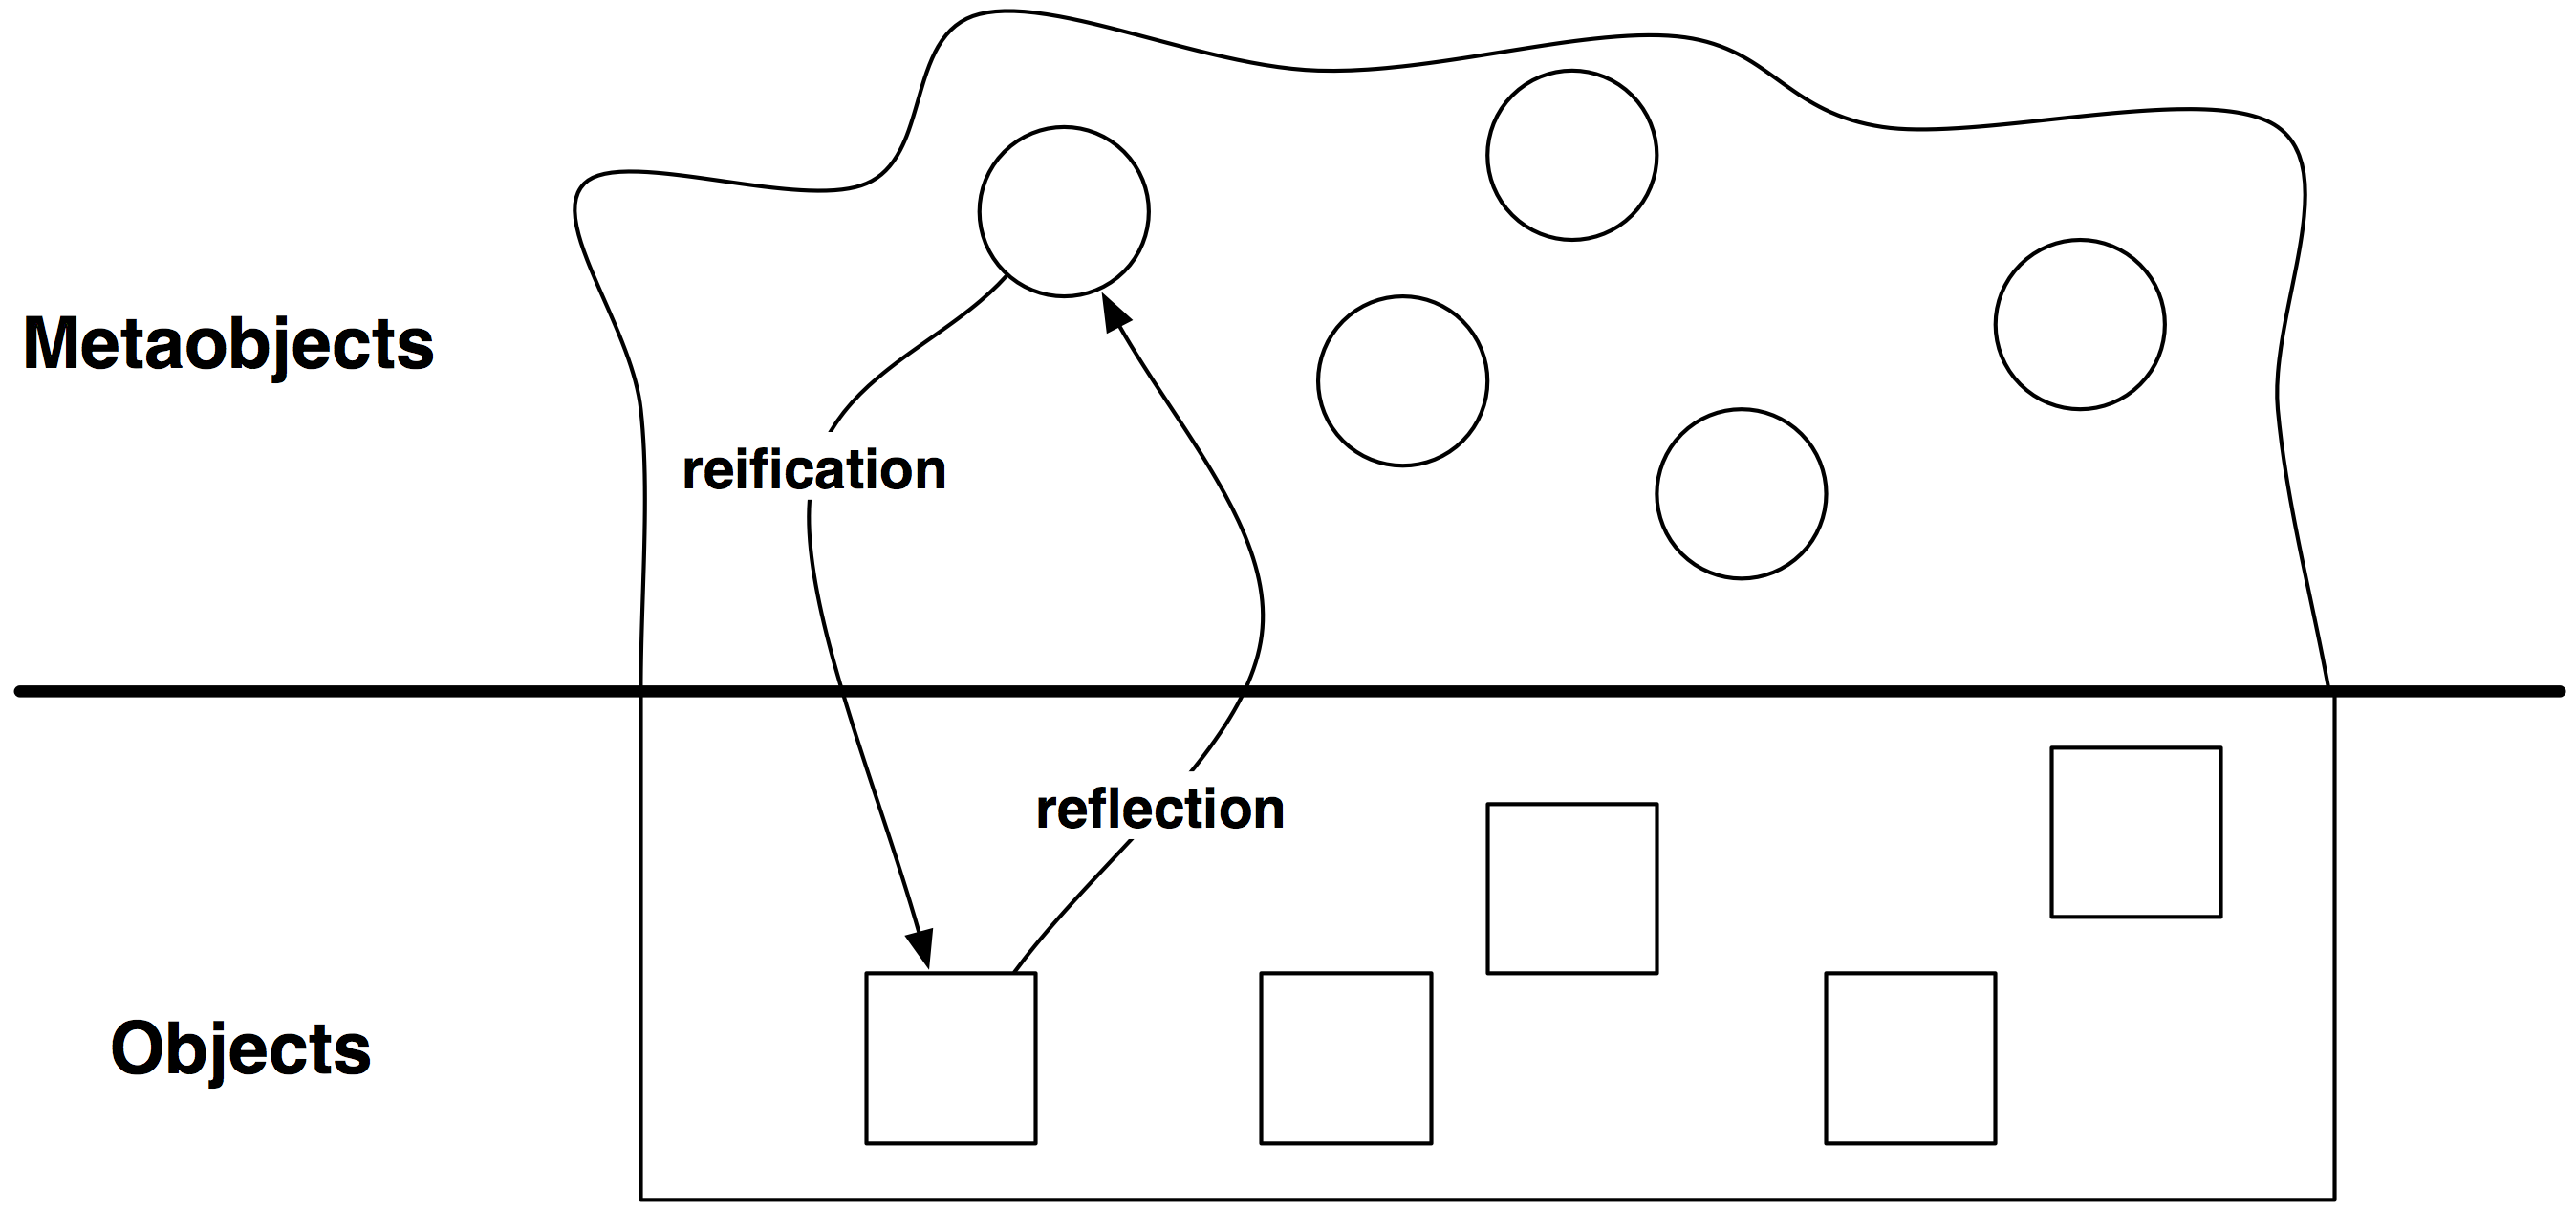
\includegraphics[width=\linewidth]{reflect}
%@	\caption{Reification and reflection.\figlabel{reflect}} % \lr{not referenced, not sure if I understand it}
	\caption{具現化とリフレクション。\figlabel{reflect}} % \lr{not referenced, not sure if I understand it}
\end{figure}

%@Conversely, it is possible in \st to modify reified metaobjects and \emph{reflect} these changes back to the runtime system (see \figref{reflect}).
逆に\st では、具現化されたメタオブジェクトを変更したり、こうした変更を実行時システムに\emph{反映}することができます(\figref{reflect}参照)。
%@This is also called \emph{intercession}, and is supported mainly by dynamic programming languages, and only to a very limited degree by static languages.
このタイプのリフレクションは、\emph{インターセッション}とも呼ばれ、主に動的なプログラミング言語がこれをサポートしますが、静的な言語では、サポートの範囲は極めて限られます。

%@A program that manipulates other programs (or even itself) is a \emphind{metaprogram}.
他のプログラム(あるいはそのプログラム自身までも)を操作するプログラムは、\emphind{メタプログラム}です。
%@For a programming language to be reflective, it should support both \ind{introspection} and \ind{intercession}.
プログラミング言語がリフレクティブであるためには、その言語は、\ind{イントロスペクション}と\ind{インターセッション}の両方をサポートしているべきです。
%@Introspection is the ability to \emph{examine} the data structures that define the language, such as objects, classes, methods and the execution stack.
イントロスペクションとは、オブジェクト、クラス、メソッド、そして実行時スタックといったデータ構造を\emph{調べる}ことができる能力のことです。これらのデータ構造は、その言語を定義するデータ構造です。
%@Intercession is the ability to \emph{modify} these structures, in other words to change the language semantics and the behavior of a program from within the program itself.
インターセッションとは、こうしたデータ構造が\emph{変更}できる、言い換えれば、言語のセマンティクスやプログラムのふるまいを、プログラム自身の中から変更できる能力のことです。
%@\emph{Structural reflection} is about examining and modifying the structures of the run-time system, and \emphind{behavioural reflection} is about modifying the interpretation of these structures.
\emph{構造的リフレクション}と言ったとき、それは、実行時システムの構造を調べ・変更することについて言うのであり、\emphind{振る舞い的リフレクション}と言ったとき、それは、これら実行時システムの構造を解釈するしかたを変更するについて言うのです。

%@In this chapter we will focus mainly on \ind{structural reflection}.
この章では、主に、\ind{構造的リフレクション}に焦点をあてます。
%@We will explore many practical examples illustrating how \st supports introspection and metaprogramming.
ここでは多くの実際的な例つまり、\st がどのようにイントロスペクションとメタプログラミングをサポートしているかを例証する、実際的な例について探ります。

%======================================
%@\section{Introspection}
\section{イントロスペクション}

%@Using the inspector, you can look at an object, change the values of its instance variables, and even send messages to it.
インスペクターを使えば、オブジェクトを詳しく見ることや、インスタンス変数の値を変更することができますし、そのオブジェクトにメッセージを送ることさえできます。

%@\dothis{Evaluate the following code in a workspace:}
\dothis{以下のコードをワークスペースで評価してみましょう:}
\begin{code}{| w |}
w := Workspace new.
w openLabel: 'My Workspace'.
w inspect
\end{code}

%@This will open a second workspace and an inspector.
こうすることによって、もうひとつのワークスペースと、インスペクターが開きます。
%@The inspector shows the internal state of this new workspace, listing its instance variables in the left part (\ct!dependents!, \ct!contents!, \ct!bindings!...) and the value of the selected instance variable in the right part.
このインスペクターは、新しく開いたワークスペースの内部状態を示しており、左側にはインスタンス変数がリストされ、(\ct!dependents!, \ct!contents!, \ct!bindings!...)そして右側には、選択されたインスタンス変数の値が表示されます。
%@The \ct!contents! instance variable represents whatever the workspace is displaying in its text area, so if you select it, the right part will show an empty string.
\ct!contents!インスタンス変数はワークスペースがそのテキスト領域に表示しているものを、それが何であれ、表わしているので、\ct!contents!を選択すれば、右側には、空文字列が表示されることになります。

\begin{figure}[ht]\centering
	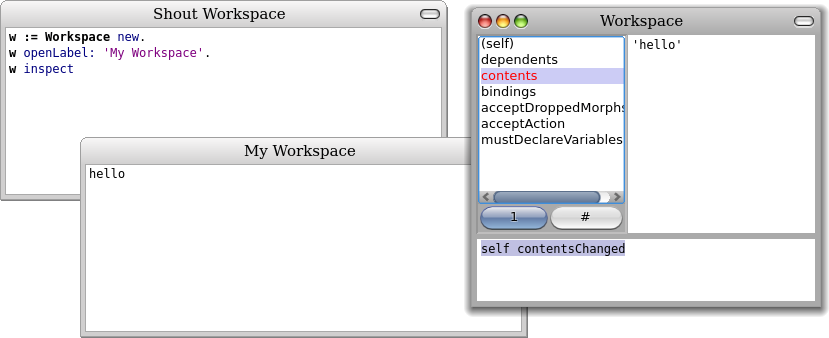
\includegraphics[width=\linewidth]{workspaceInspector}
%@	\caption{Inspecting a \ct!Workspace!.\figlabel{workspaceInspector}}
	\caption{\ct!ワークスペース!をインスペクトしている様子。\figlabel{workspaceInspector}}
\end{figure}

%@\dothis{Now type \ct!'hello'! in place of that empty string, then \emph{accept} it.}
\dothis{それでは、この空文字列のところに\ct!'hello'!と入力してから、\emph{accept}してみましょう。}
%@The value of the \ct!contents! variable will change, but the workspace window will not notice it, so it does not redisplay itself.
\ct!contents!変数の値は変りますが、ワークスペースウィンドウは、そのことに気付きません。だからワークスペースは何も再描画しません。
%@To trigger the window refresh, evaluate \ct!self contentsChanged! in the lower part of the inspector.
このウィンドウに自分自身を更新するきっかけを与えるには、インスペクターの下の部分で、\ct!self contentsChanged!を評価します。

%-----------------------------------------------------------------
%@\subsection{Accessing instance variables}
\subsection{インスタンス変数へのアクセス}

%@How does the inspector work?
インスペクターはどのように動作しているのでしょうか?
%@In \st, all instance variables are protected.
\st では、すべてのインスタンス変数は保護されています。
%@In theory, it is impossible to access them from another object if the class doesn't define any accessor.
理論上は、そのクラスが何らかのアクセサを定義していないかぎり、他のオブジェクトがこれらのインスタンス変数にアクセスすることは不可能です。
%@In practice, the inspector can access instance variables without needing accessors, because it uses the reflective abilities of \st.
実際には、インスペクターは、アクセサがなくてもインスタンス変数にアクセスすることができます。それは\st のリフレクティブな能力を用いているからです。
%@In \st, classes define instance variables either by name or by numeric indices.
\st では、クラスは、インスタンス変数を、名前か添字で定義します。
%@The inspector uses methods defined by the \ct!Object! class to access them: \lct{instVarAt: \emph{index}} and \lct{instVarNamed: \emph{aString}} can be used to get the value of the instance variable at position \lct{\emph{index}} or identified by \lct{\emph{aString}}, respectively; to assign new values to these instance variables, it uses \ct!instVarAt:put:! and \ct!instVarNamed:put:!.
インスペクターは、\ct!Object!クラスで定義されている、インスタンス変数にアクセスするためのメソッドを、用います。これら: \lct{instVarAt: \emph{index}}そして\lct{instVarNamed: \emph{aString}}は、インスタンス変数の値を得るのに用いることができます。インスタンス変数は、\lct{\emph{index}}によって位置を特定され、\lct{\emph{aString}}で識別されます。また、\ct!instVarAt:put:!や\ct!instVarNamed:put:!は、インスタンス変数に新しい値を代入するのに用います。%@?respectivelyは訳さなかった。
\mthindex{Object}{instVarAt:}
\mthindex{Object}{instVarNamed:}
\mthindex{Object}{instVarAt:put:}
\mthindex{Object}{instVarNamed:put:}

%@For instance, you can change the value of the \ct!w! binding of the first workspace by evaluating:
例えば、以下を評価すれば、最初のワークスペースで\ct!w!にバインドされたもうひとつのワークスペースオブジェクトの、内部状態を変更することができます: %@?英文が変?
\begin{code}{}
w instVarNamed: 'contents' put: 'howdy!'; contentsChanged
\end{code}

%@\important{\emph{Caveat:} Although these methods are useful for building development tools, using them to develop conventional applications is a bad idea: these reflective methods break the encapsulation boundary of your objects and can therefore make your code much harder to understand and maintain.}
\important{\emph{警告:} いくらこれらのメソッドが、開発ツールを構築するのに便利だと言っても、通常のアプリケーションを開発するのにこれらのメソッドを使うのは、悪い考えです: これらのリフレクティブなメソッドは、オブジェクトのカプセル化の境界を破り、その結果、コードは、よりわかりづらく、保守しづらいものになりかねません。}
% \lr{Why? The access does not show up when looking for all readers/writers in the code browser.}

%@Both \ct!instVarAt:! and \ct!instVarAt:put:! are \ind{primitive methods}, meaning that they are implemented as primitive operations of the \pharo virtual machine.
\ct!instVarAt:!も\ct!instVarAt:put:!も、\ind{プリミティブメソッド}であり、そのことは、これらが、\pharo 仮想マシンのプリミティブな操作によって実装されていることを意味します。
%@If you consult the code of these methods, you will see the special \ind{pragma} syntax \ct!<primitive: N>! where \ct!N! is an integer.
これらのメソッドのコードを調べれば、特殊な\ind{プラグマ}構文 \ct!<primitive: N>! が見つかるでしょう。なお、ここで、\ct!N!は整数です。
% \lr{actually this is the syntax of pragmas (method annotations), \ct!primitive:! is just a special kind of pragma}

\needlines{5}
\begin{code}{}
Object>>>instVarAt: index 
%@	"Primitive. Answer a fixed variable in an object. ..."
	"プリミティブ。オブジェクト内で固定長配列で管理されたインスタンス変数を返す。..."
	!\textbf{<primitive: 73>}!
%@	"Access beyond fixed variables."
	"固定長配列の範囲を超えた変数にアクセスする。"
	^self basicAt: index - self class instSize		
\end{code}

%@Typically, the code after the primitive invocation is not executed.
通常は、こうしたプリミティブ呼び出しのあとのコードは、実行されません。
%@It is executed only if the primitive fails. In this specific case, if we try to access a variable that does not exist, then the code following the primitive will be tried.
プリミティブ呼び出しのあとのコードは、プリミティブが失敗したときにのみ、実行されます。この\ct!instVarAt:!の例では、存在しないインスタンス変数にアクセスしようとしたとき、プリミティブに続くコードが試行されます。
%@This also allows the debugger to be started on primitive methods.
これにより、プリミティブメソッドからデバッガを開始することも可能になります。
%@Although it is possible to modify the code of primitive methods, beware that this can be risky business for the stability of your \pharo system.
いくらプリミティブメソッドのコードが変更できると言っても、そのような仕事は、\pharo システムの安定性を脅かしかねない危険な仕事であることに注意してください。%@?business: 「仕事」以外のいい訳はないか?

\begin{figure}[ht]\centering
	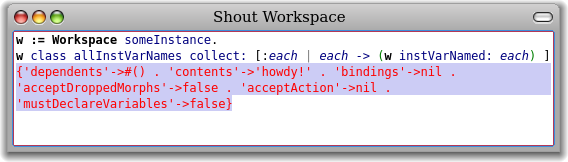
\includegraphics[width=\linewidth]{allInstanceVariables}
%@	\caption{Displaying all instance variables of a \ct!Workspace!.\figlabel{allInstanceVariables}}
	\caption{\ct!ワークスペース!のすべてのインスタンス変数を表示している様子。\figlabel{allInstanceVariables}}
\end{figure}

%@\figref{allInstanceVariables} shows how to display the values of the instance variables of an arbitrary instance (\ct!w!) of class \ct!Workspace!.
\figref{allInstanceVariables}を見れば、どのようにすれば、\ct!Workspace!クラスの任意のインスタンス (\ct!w!) のインスタンス変数が表示できるか、ということがわかります。
%@The method \ct!allInstVarNames! returns all the names of the instance variables of a given class.
この\ct!allInstVarNames!メソッドは、与えられたクラスのすべてのインスタンス変数の名前を返します。

%@In the same spirit, it is possible to gather instances that have specific properties.
同様の精神にもとづき、特定の属性を持ったインスタンスを集めることが可能です。%@?In the same spirit: 同様の精神にもとづき?
%@For instance, to get all instances of class \ct!SketchMorph! whose instance variable \ct!owner! is set to the world morph (\ie images currently displayed), try this expression:
例えば、SketchMorph!クラスのインスタンスで、\ct!owner!インスタンス変数がワールドモーフに設定されている\ct!すべてのインスタンス(\ie 現在表示されているすべてのイメージ)を得るには、次の式を試してみましょう:
\begin{code}{}
SketchMorph allInstances select: [:c | (c instVarNamed: 'owner') isWorldMorph]
\end{code}

%-----------------------------------------------------------------
%@\subsection{Iterating over instance variables}
\subsection{インスタンス変数について繰り返し処理する}

\mthindex{Object}{instanceVariableValues}
%@Let us consider the message \ct!instanceVariableValues!, which returns a collection of all values of instance variables defined by this class, excluding the inherited instance variables.
\ct!instanceVariableValues!メッセージについて考えてみましょう。これは、クラスが定義しているすべてのインスタンス変数の値のコレクションを返します。ただし、継承されたインスタンス変数は除きます。
%@For instance:
例えば:
\begin{code}{@TEST}
(1@2) instanceVariableValues --> an OrderedCollection(1 2)
\end{code}

%@The method is implemented in \ct{Object} as follows:
このメソッドは、以下のように、\ct{Object}クラスで実装されています: %@? Pharo-1.1.1には、このメソッドは無い。
\needlines{9}
\begin{code}{}
Object>>>instanceVariableValues
%@	"Answer a collection whose elements are the values of those instance variables of the receiver which were added by the receiver's class."	
	"レシーバーのクラスが追加した、すべてのレシーバーのインスタンス変数の値を要素とするコレクションを返す。"	
	| c |
	c := OrderedCollection new.
	self class superclass instSize + 1
		to: self class instSize
		do: [ :i | c add: (self instVarAt: i)].
	^ c
\end{code}

%@This method iterates over the indices of instance variables that the class defines, starting just after the last index used by the superclasses.
このメソッドは、そのクラスが定義する一連のインスタンス変数の添字について、繰り返し処理します。このときの添字は、スーパークラスで用いられていた最後の添字の直後の値から始まります。
%@(The method \ct!instSize! returns the number of all named instance variables that a class defines.)
(この\ct!instSize!メソッドは、そのクラスが定義しているすべての名前付きのインスタンス変数の数を返します。) %@? 「。)」か「)。」か?

%-----------------------------------------------------------------
%@\subsection{Querying classes and interfaces}
\subsection{クラスやインターフェースへのクエリ}

%@The development tools in \pharo (code browser, debugger, inspector...) all use the reflective features we have seen so far.
\pharo の開発ツール (コードブラウザー、デバッガー, インスペクター...)はすべて、これまでに見たリフレクティブな機能を使っています。

%@Here are a few other messages that might be useful to build development tools:
この他にももう少し、おそらく開発ツールを構築するのに便利なメッセージがあります:

%@\lct{isKindOf: \emph{aClass}} returns true if the receiver is instance of \lct{\emph{aClass}} or of one of its superclasses.
\lct{isKindOf: \emph{aClass}}は、レシーバーが\lct{\emph{aClass}}や、そのスーパークラスのいずれかのインスタンスであるときに、trueを返します。
%@For instance:
例えば:
\begin{code}{@TEST}
1.5 class                     --> Float
1.5 isKindOf: Number --> true
1.5 isKindOf: Integer   --> false
\end{code}
\mthindex{Object}{class}
\mthindex{Object}{isKindOf:}

%@\lct{respondsTo: \emph{aSymbol}} returns true if the receiver has a method whose selector is \lct{\emph{aSymbol}}.
\lct{respondsTo: \emph{aSymbol}}は、レシーバーのクラスに、セレクターが\lct{\emph{aSymbol}}であるようなメソッドが定義されているときに、trueを返します。%@?receiver has a method: 「レシーバーのクラス」というように「クラス」を補った。
%@For instance:
例えば:
\needlines{3}
\begin{code}{@TEST}
%@1.5 respondsTo: #floor      --> true    "since Number implements floor"
1.5 respondsTo: #floor      --> true    "Numberがfloorを実装しているので"
1.5 floor                            --> 1
%@Exception respondsTo: #, --> true    "exception classes can be grouped"
Exception respondsTo: #, --> true    "例外クラスはグループ化することができる"
\end{code}
\mthindex{Object}{respondsTo:}

%@\important{\emph{Caveat:} Although these features are especially useful for defining development tools, they are normally not appropriate for typical applications.
\important{\emph{警告:}いくらこれらの機能が、とりわけ開発ツールを定義するのに便利だからと言っても、これらは通常、典型的なアプリケーションには適していません。
%@Asking an object for its class, or querying it to discover which messages it understands, are typical signs of design problems, since they violate the principle of encapsulation.
オブジェクトに、それが属するクラスを尋ねたり、オブジェクトがどのようなメッセージを理解するかを見つけ出そうと、それにクエリを送ること、設計上の欠陥を典型的に示すものです。なぜならそれは、カプセル化の原則を破るからです。%@?少し日本語が変?
%@Development tools, however, are not normal applications, since their domain is that of software itself. As such these tools have a right to dig deep into the internal details of code.}
開発ツールは、しかしながら、通常のアプリケーションではありません。なぜなら、開発ツールは、ソフトウェアそれ自身を対象領域とするものだからです。それで、これらのツールは、コードの内部の詳細について、深く掘り下げることを許されているのです。}

%There also exist mechanisms for introspecting on various parts of the run-time system, such as  the process scheduler, the memory manager and so on. For now we will focus on navigating through objects, classes and methods, and we will look more closely at rest of the runtime system in an other chapter.
%\on{let's not mention this if we don't actually write such a chapter!}

%-----------------------------------------------------------------
%@\subsection{Code metrics}
\subsection{コードメトリクス}

%@Let's see how we can use \st's introspection features to quickly extract some code metrics.
\st のイントロスペクション機能をどのように使えば、いくつかのコードメトリクスが、手早く抽出できるか、見てみましょう。
%@Code \ind{metrics} measure such aspects as the depth of the inheritance hierarchy, the number of direct or indirect subclasses, the number of methods or of instance variables in each class, or the number of locally defined methods or instance variables.
コード\ind{メトリクス}は、次のようなコードの側面を測ります --- 継承の階層の深さ、直接・間接のサブクラスの数、各クラスのメソッドやインスタンス変数の数、局所的に定義されたメソッドやインスタンス変数の数。
%@Here are a few metrics for the class \ct!Morph!, which is the superclass of all graphical objects in \pharo, revealing that it is a huge class, and that it is at the root of a huge hierarchy. Maybe it needs some refactoring! 
以下に、\ct!Morph!クラスのメトリクスをいくつか挙げます。\ct!Morph!クラスは、\pharo においては、すべてのグラフィカルなオブジェクトのスーパークラスです。このメトリクスにより、このクラスが巨大なクラスであり、巨大な階層のルートであることが明かになります。何らかのリファクタリングが必要なのかもしれません! 

\mthindex{Behavior}{allSuperclasses}
\mthindex{Behavior}{allSelectors}
\mthindex{Behavior}{allInstVarNames}
\mthindex{Behavior}{selectors}
\mthindex{Behavior}{instVarNames}
\mthindex{Behavior}{subclasses}
\mthindex{Behavior}{allSubclasses}
\mthindex{ClassDescription}{linesOfCode}
\begin{code}{}
%@Morph allSuperclasses size.  -->       2 "inheritance depth"
Morph allSuperclasses size.  -->       2 "インヘリタンスの深さ"
%@Morph allSelectors size.        --> 1378 "number of methods"
Morph allSelectors size.        --> 1378 "メソッドの数"
%@Morph allInstVarNames size. -->      6 "number of instance variables"
Morph allInstVarNames size. -->      6 "インスタンス変数の数"
%@Morph selectors size.             -->  998 "number of new methods"
Morph selectors size.             -->  998 "Morphで新しく定義されたメソッドの数"
%@Morph instVarNames size.     -->      6 "number of new variables"
Morph instVarNames size.     -->      6 "Morphで新しく定義されたインスタンス変数メソッドの数"
%@Morph subclasses size.          -->    45 "direct subclasses"
Morph subclasses size.          -->    45 "直接のサブクラスの数"
%@Morph allSubclasses size.      -->  326 "total subclasses"
Morph allSubclasses size.      -->  326 "サブクラスの総数"
%@Morph linesOfCode.               --> 5968 "total lines of codeBANG"
Morph linesOfCode.               --> 5968 "総コード行数"
\end{code}

%@One of the most interesting metrics in the domain of object-oriented languages is the number of methods that extend methods inherited from the superclass.
オブジェクト指向言語のドメインにおいて、最も興味深いメトリクスのひとつは、どのくらいの数のメソッドが、スーパークラスから継承したメソッドを拡張しているかということです。
%@This informs us about the relation between the class and its superclasses.
このことにより、クラスとそのスーパークラスの関係を知ることができます。
%@In the next sections we will see how to exploit our knowledge of the runtime structure to answer such questions.
次の節では、その種のメトリクスに関する疑問にどう答えるか、つまり実行時構造に関するこれまでの知識をフルに使ってどう答えるか、について示します。%@?will see: 示します? our knowledge: これまでの知識

%======================================
%@\section{Browsing code}
\section{コードをブラウズする}

%@In \st, everything is an object. In particular, classes are objects that provide useful features for navigating through their instances.
\st では、すべてがオブジェクトです。とくにクラスは、クラスのインスタンスの世界をナビゲートするための、便利な機能を提供するオブジェクトです。%@?navigating through their instances: クラスのインスタンスの世界をナビゲートするための?
%@Most of the messages we will look at now are implemented in \ct{Behavior}, so they are understood by all classes.
これから詳しく見るメッセージの多くは、\ct{Behavior}で実装されているので、これらのメッセージは、すべてのクラスが、これを理解することができます。

%@As we saw previously, you can obtain an instance of a given class by sending it the message \ct!#someInstance!.
以前見たように、与えられたクラスのインスタンスは、そのクラスにメッセージ: \ct!#someInstance!メッセージを送ることにより、得ることができます。%@?As we saw previouslyだと!?
\mthindex{Behavior}{someInstance}
\begin{code}{@TEST} % Possibly fragile!
Point someInstance --> 0@0
\end{code}

%@You can also gather all the instances with \ct!#allInstances!, or the number of alive instances in memory with \ct!#instanceCount!.
また、すべてのインスタンスを集めるのに、\ct!#allInstances!を用いることができ、また、メモリ中で生きているインスタンスの数を得るのに、\ct!#instanceCount!を用いることができます。

\alex{In a Pharo0.1-10342dev09.96.3, I have "ByteString instanceCount --> 63607"}
\mthindex{Behavior}{allInstances}
\mthindex{Behavior}{instanceCount}
\mthindex{Behavior}{allSubInstances}
\begin{code}{} % Cannot test this
ByteString allInstances        --> #('collection' 'position'  ...)
ByteString instanceCount    --> 104565
String allSubInstances size -->  101675
\end{code}

%@These features can be very useful when debugging an application, because you can ask a class to enumerate those of its methods exhibiting specific properties.
以下の機能は、アプリケーションをデバッグするときに、非常に便利なことがあります。なぜなら、クラスに対して、そのメソッド --- 具体的な属性を示すメソッドを列挙するよう依頼することができるからです。%@?exhibitingは何にかかる?
\begin{itemize}
%@\item \mthind{Behavior}{whichSelectorsAccess:} returns the list of all selectors of methods that read or write the instance variable named by the argument
\item \mthind{Behavior}{whichSelectorsAccess:} 引数が示すインスタンス変数を読み書きするすべてのメソッドセレクターのリストを返す %@?selectors of methods: メソッドセレクター? 他にも、method selector, method's selectorの原語が発見されている。
%@\item \mthind{Behavior}{whichSelectorsStoreInto:} returns the selectors of methods that modify the value of an instance variable
\item \mthind{Behavior}{whichSelectorsStoreInto:} インスタンス変数の値を変更するメソッドセレクターを返す
%@\item \mthind{Behavior}{whichSelectorsReferTo:} returns the selectors of methods that send a given message
\item \mthind{Behavior}{whichSelectorsReferTo:} 与えられたメッセージを送るメッセージセレクターを返す
%@\item \mthind{Behavior}{crossReference} associates each message with the set of methods that send it.
\item \mthind{Behavior}{crossReference} 各メッセージを、そのメッセージを送るメソッドの集合に関連づける %@?Method Finderで探したが、crossReferenceというメソッドは見つからなかった。
\end{itemize}

\begin{code}{} % TOO FRAGILE TO TEST
Point whichSelectorsAccess: 'x'    --> an IdentitySet(#'\\' #= #scaleBy: ...)
Point whichSelectorsStoreInto: 'x' --> an IdentitySet(#setX:setY: ...)
Point whichSelectorsReferTo: #+  --> an IdentitySet(#rotateBy:about: ...)
Point crossReference --> an Array(
		an Array('*' an IdentitySet(#rotateBy:about: ...))
		an Array('+' an IdentitySet(#rotateBy:about: ...))
		...)
\end{code}

%@The following messages take inheritance into account:
以下のメッセージは、継承に着眼します: %@?take inheritance into account: 継承に着眼?
\begin{itemize}
%@\item \mthind{Behavior}{whichClassIncludesSelector:} returns the superclass that implements the given message
\item \mthind{Behavior}{whichClassIncludesSelector:} 与えられたメッセージを実装するスーパークラスを返す
%@\item \mthind{Behavior}{unreferencedInstanceVariables} returns the list of instance variables that are neither used in the receiver class nor any of its subclasses
\item \mthind{Behavior}{unreferencedInstanceVariables}レシーバークラスでも、そのどのサブクラスでも使われない、インスタンス変数のリストを返す
\end{itemize}

\begin{code}{@TEST}
Rectangle whichClassIncludesSelector: #inspect --> Object
Rectangle unreferencedInstanceVariables            --> #()
\end{code}

%@\clsind{SystemNavigation} is a facade that supports various useful methods for querying and browsing the source code of the system.
\clsind{SystemNavigation}は、さまざまな便利なメソッドをサポートする、ファサードです。ここで言うメソッドとは、システムのソースコードにクエリを送ったり、ソースコードをブラウズするのに便利なメソッドのことです。
%@\ct{SystemNavigation} \mthind{SystemNavigation class}{default} returns an instance you can use to navigate the system.
\ct{SystemNavigation} \mthind{SystemNavigation class}{default}は、システムをナビゲートするのに使えるインスタンスを返します。
%@For example:
例えば:

\mthindex{SystemNavigation}{allClassesImplementing:}
\begin{code}{@TEST}
SystemNavigation default allClassesImplementing: #yourself --> {Object}
\end{code}

%@The following messages should also be self-explanatory:
以下のメッセージの意味も、字面から明かでしょう:

\mthindex{SystemNavigation}{allSentMessages}
\mthindex{SystemNavigation}{allUnsentMessages}
\mthindex{SystemNavigation}{allUnimplementedCalls}
\begin{code}{}
SystemNavigation default allSentMessages size          --> 24930
SystemNavigation default allUnsentMessages size      --> 6431
SystemNavigation default allUnimplementedCalls size --> 270
\end{code}

%@Note that messages implemented but not sent are not necessarily useless, since they may be sent implicitly (\eg using \ct{perform:}).
ここで次のことに注意してください。実装されてはいても送られないメッセージは、かならずしも用なし、ということではありません。なぜなら、それらは間接的に送られることもありうるからです(\eg \ct{perform:}を使って)。
%@Messages sent but not implemented, however, are more problematic, because the methods sending these messages will fail at runtime.
送られるのに実装されていないメッセージには、しかしながら、もっと問題があります。なぜなら、これらのメッセージを送るメソッドは、いずれ実行時に失敗することになるからです。
%@They may be a sign of unfinished implementation, obsolete APIs, or missing libraries.
これらは、未完了の実装、廃止されたAPI、あるいはライブラリの欠落の兆候でしょう。

\mthindex{SystemNavigation}{allCallsOn:}
%@\ct!SystemNavigation default allCallsOn: #Point! returns all messages sent explicitly to \ct!Point! as a receiver.
\ct!SystemNavigation default allCallsOn: #Point! は、\ct!Point!レシーバーに明示的に送られるメッセージを返します。

%@All these features are integrated in the programming environment of \pharo, in particular in the code browsers.
これらすべての機能は、\pharo のプログラミング環境、とくにコードブラウザー、に統合されています。
%@As you are surely already aware, there are convenient keyboard shortcuts for browsing all i\underline{m}plementors (\short{m}) and se\underline{n}ders (\short{n}) of a given message.
すでにきっとお気付きでしょうが、次のような便利なキーボードショートカットがあります: すべてのインプリメンター(i\underline{m}plementors)をブラウズするための (\short{m})、そして、与えられたメッセージのセンダー(se\underline{n}ders)をブラウズするための (\short{n})。
%@What is perhaps not so well known is that there are many such pre-packaged queries implemented as methods of the \ct{SystemNavigation} class in the \prot{browsing} protocol.
おそれく次のことは、それほどよく知られていないでしょう。このようなパッケージ済みのたくさんのクエリが、\ct{SystemNavigation}クラスの\prot{browsing}プロトコルのメソッドとして実装されています。%@?browsingプロトコル? browseではないのか(Pharo-1.1.1)?
%@For example, you can programmatically browse all implementors of the message \ct{ifTrue:} by evaluating:
例えば、プログラム的に\ct{ifTrue:}メッセージのすべてのインプリメンターをブラウズするのは、以下を評価することで可能です:
\mthindex{SystemNavigation}{browseAllImplementorsOf:}
\begin{code}{}
SystemNavigation default browseAllImplementorsOf: #ifTrue:
\end{code}

\begin{figure}[ht]\centering
	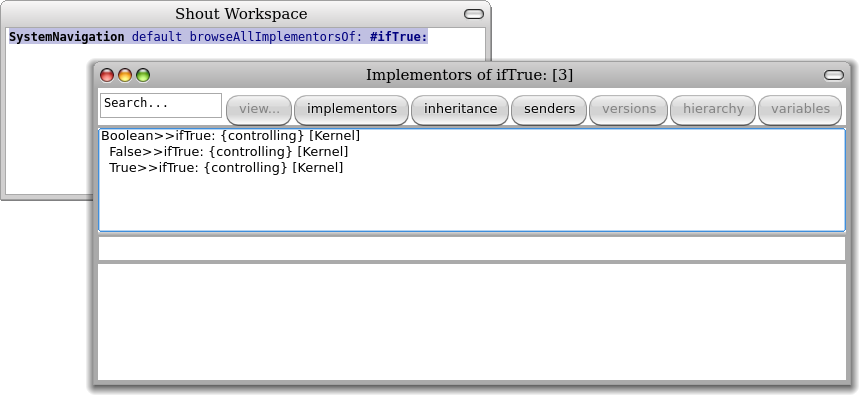
\includegraphics[width=\linewidth]{implementors}
%@	\caption{Browse all implementations of \ct!\#ifTrue:!.\figlabel{implementors}}
	\caption{すべての\ct!\#ifTrue:の実装をブラウズしている様子。\figlabel{implementors}}
\end{figure}

%@Particularly useful are the methods \ct{browseAllSelect:} and \lct{browseMethodsWithSourceString:}.  Here are two different ways to browse all methods in the system that perform super sends (the first way is rather brute force; the second way is better and eliminates some false positives):
とりわけ便利なのは、\ct{browseAllSelect:}メソッドと\lct{browseMethodsWithSourceString:}メソッドです。以下に述べるのは、システム中のすべてのメソッドのうち、super-送信を行うものをブラウズする、ふたつの異った方法です (最初の方法は、かなり総当たり式の方法です; 2番目の方法は、より好ましくいもので、偽陽性の結果をいくつか除外することができます): %@?false positives: 偽陽性の結果?
\mthindex{SystemNavigation}{browseMethodsWithSourceString:}
\mthindex{SystemNavigation}{browseAllSelect:}
\begin{code}{}
SystemNavigation default browseMethodsWithSourceString: 'super'.
SystemNavigation default browseAllSelect: [:method | method sendsToSuper ].
\end{code}

%======================================
%@\section{Classes, method dictionaries and methods}
\section{クラス、メソッド辞書、そしてメソッド}

%@Since classes are objects, we can inspect or explore them just like any other object.
クラスはオブジェクトなので、他のオブジェクトとまったく同様、クラスをインスペクトやエクスプロアすることもできます。

\mthindex{Object}{explore}
%@\dothis{Evaluate \ct{Point explore}.}
\dothis{\ct{Point explore}を評価してみましょう。}

%@In \figref{CompiledMethod}, the \ind{explorer} shows the structure of class \clsind{Point}.
\figref{CompiledMethod}が示しているのは、\ind{エクスプローラー}が、\clsind{Point}クラスの構造を示している様子です。
%@You can see that the class stores its methods in a dictionary, indexing them by their selector.
ここでは、クラスがそのメソッドを辞書に格納していることが確認できます。セレクターが、辞書の見出しになっています。
%@The selector \ct{#*} points to the decompiled \ind{bytecode} of \ct!Point>>>*!.
The selector \ct{#*}セレクターは、逆コンパイルされた\ct!Point>>>*の\ind{バイトコード}を指しています。

\begin{figure}[ht]\centering
	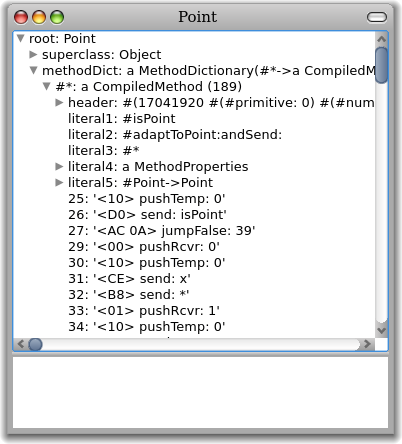
\includegraphics[width=.5\linewidth]{CompiledMethod}
%@	\caption{Explorer class \ct!Point! and the bytecode of its \ct!\#*! method.\figlabel{CompiledMethod}}
	\caption{\ct!Point!クラスと\ct!Point!クラスの\ct!\#*!メソッドをエクスプロアする。\figlabel{CompiledMethod}} %@?Explorer: なぜ名詞?
\end{figure}

%@Let us consider the relationship between classes and methods.
クラスとメソッドの関係について考えてみましょう。
%@In \figref{MethodsAsObjects} we see that classes and metaclasses have the common superclass \ct{Behavior}. This is where \mthind{Behavior}{new} is defined, amongst other key methods for classes.
\figref{MethodsAsObjects}で、クラスとメタクラスには共通のスーパークラス---\ct{Behavior}があることを見ました。\ct{Behavior}クラスで、\mthind{Behavior}{new}が定義されています。newはクラスの他の主要なメソッドのひとつにすぎません。%@?最後のnewをマークアップするか? %@?among other things/places/factors etc: used to say that you are only mentioning one or two people or things out of a much larger group: (LDOCE) 
%@Every class has a method dictionary, which maps method selectors to \ind{compiled methods}.
どのクラスにもメソッド辞書があって、メソッド辞書は、メソッドセレクターと\ind{コンパイル済みメソッド}を、対応づけます。
%@Each compiled method knows the class in which it is installed.
コンパイル済みメソッドはそれぞれ、そのメソッドがインストールされているクラスを知っています。
%@In \figref{CompiledMethod} we can even see that this is stored in an association in \ct{literal5}.
\figref{CompiledMethod}を見れば、このPointクラスが、\ct!\#*!に当たるコンパイル済みメソッドの、\ct{literal5}というインスタンス変数に、アソシエーションとして格納されていることがわかります。

\begin{figure}[ht]\centering
	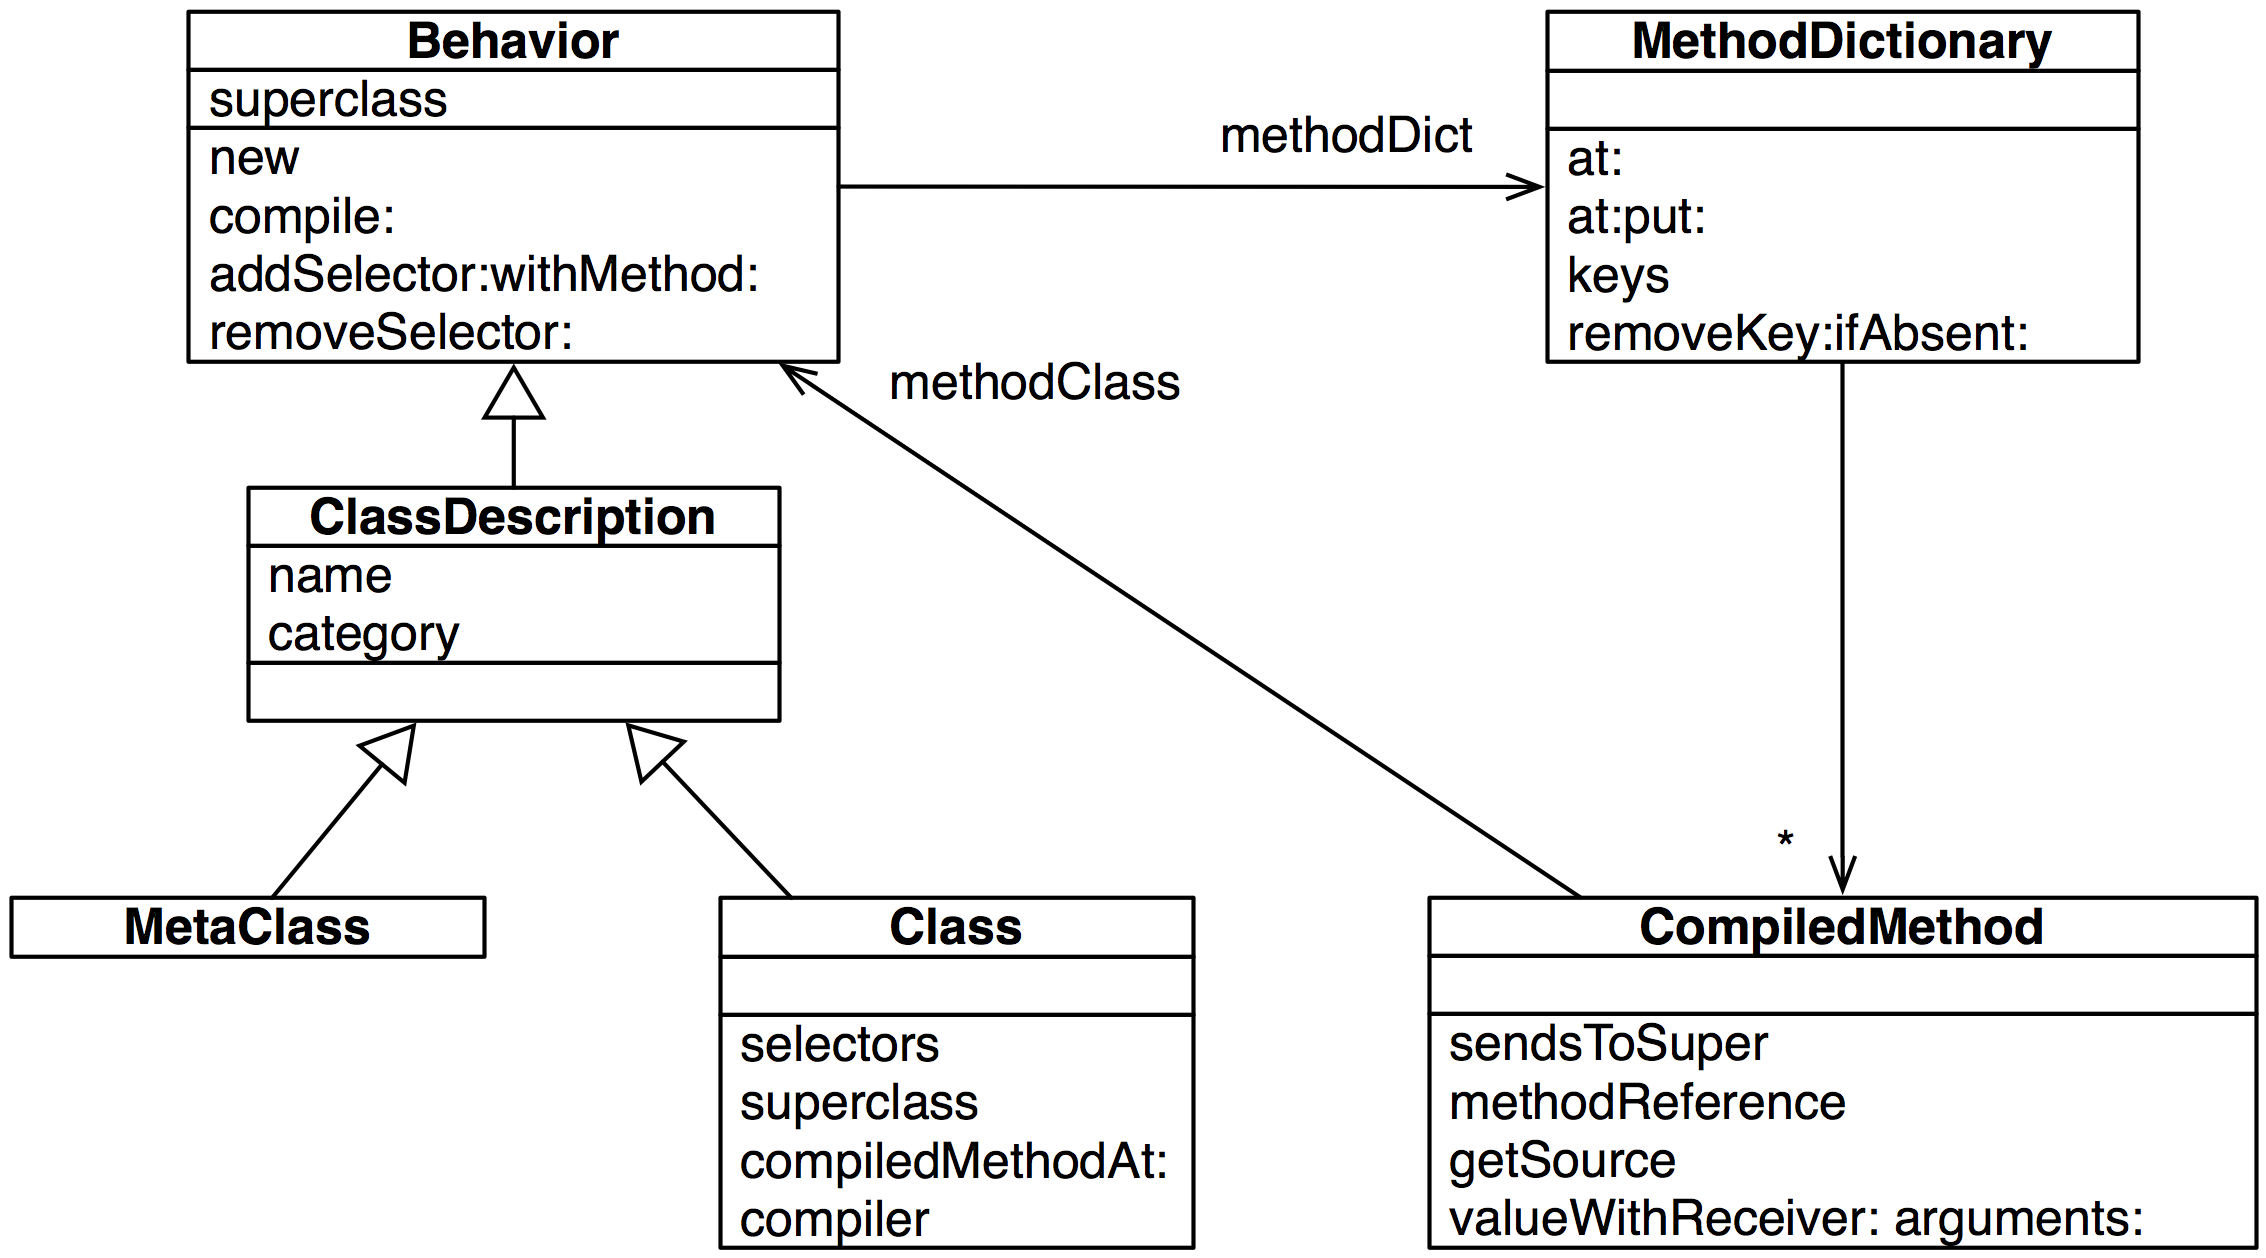
\includegraphics[width=\linewidth]{MethodsAsObjects}
%@	\caption{Classes, method dictionaries and compiled methods\figlabel{MethodsAsObjects}}
	\caption{クラス、メソッド辞書、そしてコンパイル済みメソッド\figlabel{MethodsAsObjects}}
\end{figure}

%@We can exploit the relationships between classes and methods to pose queries about the system.
クラスとメソッドの関係をフルに使って、\pharo のシステムについてのクエリを送ることができます。
%@For example, to discover which methods are newly introduced in a given class, \ie do not override superclass methods, we can navigate from the class to the \ind{method dictionary} as follows:
例えば、どのメソッドが、与えられたクラスに新規に導入されたかということを見出すことは、\ie どのメソッドが、スーパークラスのメソッドをオーバーライドしていないか、ということは見出すことは、以下のように、クラスから\ind{メソッド辞書}をナビゲートすることで可能になります: %@?少し日本語が変。
\mthindex{Behavior}{methodDict}
\begin{code}{}
[:aClass| aClass methodDict keys select: [:aMethod |
  (aClass superclass canUnderstand: aMethod) not ]] value: SmallInteger
  --> an IdentitySet(#threeDigitName #printStringBase:nDigits: ...)
\end{code}

%@A compiled method does not simply store the bytecode of a method.
コンパイル済みメソッドは、単に、メソッドのバイトコードを格納しているだけではありません。
%@It is also an object that provides numerous useful methods for querying the system.
コンパイル済みメソッド自身がまた、システムにクエリを送るための、多数の便利なメソッドを提供するオブジェクトなのです。
%@One such method is \ct{isAbstract} (which tells if the method sends \ct{subclassResponsibility}).
そのようなメソッドのひとつに、\ct{isAbstract}があります(\ct{isAbstract}メソッドは、コンパイル済みメソッドが、\ct{subclassResponsibility}を送るかどうか、教えてくれます)。
%@We can use it to identify all the abstract methods of an abstract class
\ct{isAbstract}メソッドを使えば、抽象クラスのすべての抽象メソッドを識別することができます。
\needlines{4}
\begin{code}{}
[:aClass| aClass methodDict keys select: [:aMethod |
  (aClass>>aMethod) isAbstract ]] value: Number
  --> an IdentitySet(#storeOn:base: #printOn:base: #+ #- #* #/ ...)
\end{code}
%@Note that this code sends the \ct{>>} message to a class to obtain the compiled method for a given selector.
このコードでは、次のことに注意してください。クラスに対して、\ct{>>}メッセージが送られ、その結果、与えられたセレクターに対するコンパイル済みメソッドが得られています。

% As a slightly more complex example, we can browse 

%@To browse the super-sends within a given hierarchy, for example within the Collections hierarchy, we can pose a more sophisticated query:
与えられた階層内のsuper-送信をブラウズするには、例えば、Collectionの階層内のsuper-送信をブラウズするには、より洗練されたクエリを送ることができます:
\begin{code}{}
class := Collection.
SystemNavigation default
  browseMessageList: (class withAllSubclasses gather: [:each |
    each methodDict associations
      select: [:assoc | assoc value sendsToSuper]
      thenCollect: [:assoc | MethodReference class: each selector: assoc key]])
  name: 'Supersends of ' , class name , ' and its subclasses'
\end{code}
%@Note how we navigate from classes to method dictionaries to compiled methods to identify the methods we are interested in.
関心のあるメソッド(super-送信をするメソッド)を識別するために、クラスからメソッド辞書へと、そしてメソッド辞書からコンパイル済みメソッドへと、どのようにナビゲートしているかに注意してください。
%@A \ct{MethodReference} is a lightweight proxy for a compiled method that is used by many tools.
\ct{MethodReference}は、コンパイル済みメソッドのための軽量のプロキシーで、たくさんのツールがこのプロキシーを使っています。
%@There is a convenience method \clsmthind{CompiledMethod}{methodReference} to return the method reference for a compiled method.
\clsmthind{CompiledMethod}{methodReference}という簡便メソッドがあって、これは、コンパイル済みメソッドに対するメソッド参照を返します。%@?convenience: 簡便?
\begin{code}{@TEST}
(Object>>#=) methodReference methodSymbol --> #=
\end{code}

%======================================
%@\section{Browsing environments}
\section{ブラウジング環境}

%@Although \clsind{SystemNavigation} offers some useful ways to programmatically query and browse system code, there is a better way.  The \ind{Refactoring Browser}, which is integrated into \pharo, provides both interactive and programmatic ways to pose complex queries.
\clsind{SystemNavigation}は、システムコードに対してプログラム的にクエリを送り、プログラム的にこれをブラウズする方法をいくつか提供しますが、もっとよい方法があります。\pharo には\ind{Refactoring Browser}というものが統合されているのですが、これを使えば、複雑なクエリを、会話的にもプログラム的にも送ることができます。

%@Suppose we are interested to discover which methods in the \lct{Collection} hierarchy send a message to \super which is different from the method's selector.
\lct{Collection}の階層のメソッドのうち、どのようなメソッドが、そのセレクターと異なるメッセージを\super に送っているか、それを見出すことに関心があったとしましょう。
%@This is normally considered to be a bad \ind{code smell}, since such a \super-send should normally be replaced by a \self-send. (Think about it --- you only \emph{need} \super to extend a method you are overriding; all other inherited methods can be accessed by sending to \self!)
このように、何かをオーバーライドしているわけではないメソッドが、\super-送信をしているのは、通常は、悪い\ind{コード臭}と考えられます。なぜなら、そのような\super-送信は、通常は、\self-送信で置き換えられるべきだからです。(次のことを考えてみてください --- \super は、メソッドをオーバーライドしようとするときにだけ\emph{必要}です; 他のすべての継承されたメソッドにアクセスするには、\selfにメッセージを送ることで済みます!)

%@The refactoring browser provides us with an elegant way to restrict our query to just the classes and methods we are interested in.
リファクタリングブラウザーというツールは、クエリの送り先を、関心のあるクラスやメソッドに限定するための、エレガントな方法を提供します。

%@\dothis{Open a browser on the class \ct{Collection}.
\dothis{ブラウザーを開けて、\ct{Collection}.を見てみましょう。
%@\actclick on the class name and select \menu{refactoring scope>subclasses with}.
クラス名を\actclick して、\menu{refactoring scope>subclasses with}を選択しましょう。
%@This will open a new Browser Environment on just the \ct{Collection} hierarchy.
こうすると、まさに、\ct{Collection}階層についてのブラウザー環境が、新規に開きます。 
%@Within this restricted scope select \menu{refactoring scope>super-sends} to open a new environment with all methods that perform super-sends within the \ct{Collection} hierarchy.
この限定されたスコープの中で、\menu{refactoring scope>super-sends}を選択しましょう。すると、新しいウィンドウが開き、\ct{Collection}階層の中で、super-送信を行っているすべてのメソッドが列挙されます。
%@Now \click on any method and select \menu{refactor>code critics}.
さあ、任意のメソッドを\click し、\menu{refactor>code critics}を選んでみましょう。
%@Navigate to \menu{Lint checks>Possible bugs>Sends different super message} and \actclick to select \menu{browse}.}
\menu{Lint checks>Possible bugs>Sends different super message}とナビゲートして、\menu{browse}を\actclick してみましょう。}

%@In \figref{sendDifferentSuper} we can see that 19 such methods have been found within the \ct{Collection} hierarchy, including \ct{Collection>>>printNameOn:}, which sends \ct{super printOn:}.
\figref{sendDifferentSuper}では、そのような19個のメソッドが、\ct{Collection}階層の中に見つかったのを見ることができます。それらの中には、\ct{Collection>>>printNameOn:} があって、このメソッドは、\ct{super printOn:}を送っています。
\begin{figure}[ht]\centering
	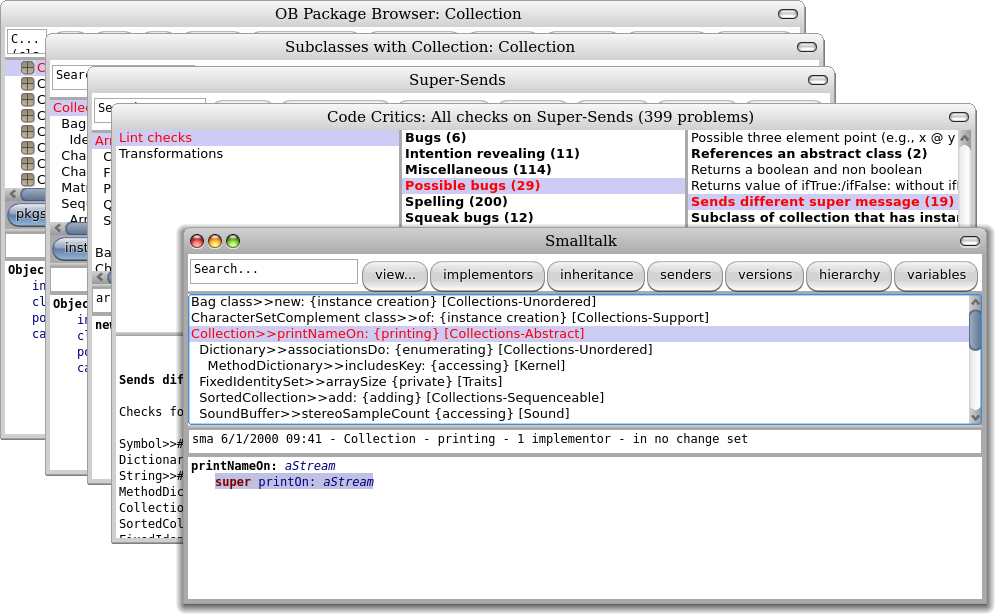
\includegraphics[width=\linewidth]{sendDifferentSuper}
%@	\caption{Finding methods that send a different super message.\figlabel{sendDifferentSuper}}
	\caption{自身のセレクターとは違うメッセージを、superに送っているメソッドを、見つけている様子。\figlabel{sendDifferentSuper}}
\end{figure}

%@Browser environments can also be created programmatically.
ブラウザー環境はまた、プログラム的に作ることができます。
%@Here, for example, we create a new \clsind{BrowserEnvironment} for \clsind{Collection} and its subclasses, select the super-sending methods, and open the resulting environment.
例えば、以下のように、\clsind{Collection}とそのサブクラスに対する、新しい\clsind{BrowserEnvironment}のインスタンスを生成し、このインスタンスに対して\ct!selectMethods:!を用いて、superを送っているメソッドを抽出し、結果を\ct{SelectorEnvironment}オブジェクトとして表示することができます。
\needlines{4}
\begin{code}{}
((BrowserEnvironment new forClasses: (Collection withAllSubclasses))
	selectMethods: [:method | method sendsToSuper])
	label: 'Collection methods sending super';
	open.
\end{code}{}

%@Note how this is considerably more compact than the earlier, equivalent example using \ct{SystemNavigation}.
この例は、先程の例、つまり\ct{SystemNavigation}を用いたこれと等価な例より、かなりコンパクトになっていることに注意してください。

%@Finally, we can find just those methods that send a different super message programmatically as follows:
最終的に、このようなメソッド、つまり異なったsuperメッセージを送っているメソッドを、以下のようにして、プログラム的に見つけ出すことができます:
\needlines{6}
\begin{code}{}
((BrowserEnvironment new forClasses: (Collection withAllSubclasses))
	selectMethods: [:method | 
		method sendsToSuper
		and: [(method parseTree superMessages includes: method selector) not]])
	label: 'Collection methods sending different super';
	open
\end{code}
%@Here we ask each compiled method for its (Refactoring Browser) parse tree, in order to find out whether the super messages differ from the method's selector.
ここでは、各コンパイル済みメソッドに、その (Refactoring Browser) 解析木について尋ね、superメッセージが、メソッドセレクターと異なっているかを探り出しています。
%@Have a look at the \prot{querying} protocol of the class \ct{RBProgramNode} to see some the things we can ask of parse trees.
\ct{RBProgramNode}クラスの\prot{querying}プロトコルを見てみましょう。これを見れば、解析木に対して、何が聞けるかがわかります。%@?see some the things?

%======================================
%@\section{Accessing the run-time context}
\section{実行時コンテクストにアクセスする}

%@We have seen how \st's reflective capabilities let us query and explore objects, classes and methods.  But what about the run-time environment?
これまで、\st のリフレクティブな機能により、オブジェクト、クラス、メソッドにクエリを送ったり、これらをエクスプロアしたりできることを見てきました。しかし、実行時環境についてはどうでしょう?

%-----------------------------------------------------------------
%@\subsection{Method contexts}
\subsection{メソッドコンテクスト}

%@In fact, the run-time context of an executing method is in the virtual machine --- it is not in the image at all!
実際、実行中のメソッドの実行時コンテクストは、仮想マシンの中にあります --- 決して、イメージの中ではない、ということです!
%@On the other hand, the \ind{debugger} obviously has access to this information, and we can happily explore the run-time context, just like any other object.
その一方で、\ind{デバッガー}はもちろん、この実行時コンテクストにアクセスすることができます。そして幸運なことに、この実行時コンテクストをエクスプロアすることができます。それはちょうど、他の任意のオブジェクトをエクスプロアすることができるのと同様です。
%@How is this possible?
これは、どのようにして可能なのでしょうか?

%@Actually, there is nothing magical about the debugger.
実は、デバッガーには何の魔法もありません。
%@The secret is the pseudo-variable \pvind{thisContext}, which we have encountered only in passing before.
秘密は、\pvind{thisContext}という疑似変数にあって、%@?which~: 意味不明。
%@Whenever \ct{thisContext} is referred to in a running method, the entire run-time context of that method is reified and made available to the image as a series of chained \clsind{MethodContext} objects.
実行中のメソッドが\ct{thisContext}を参照したとき、そのメソッドの完全な実行時コンテクストが具現化され、\clsind{MethodContext}オブジェクトの一連の連鎖として、仮想イメージから利用できるようになります。

%@We can easily experiment with this mechanism ourselves.
このメカニズムについて、簡単に、自分自身で実験することができます。

%@\dothis{Change the definition of \ct{Integer>>>factorial} by inserting the underlined expression as shown below:}
\dothis{\ct{Integer>>>factorial}の定義を変えてみましょう。以下のようにします:}

\mthindex{Object}{halt}
\begin{code}{}
Integer>>>factorial
%@	"Answer the factorial of the receiver."
	"レシーバーの階乗を返す。"
	self = 0 ifTrue: [!\underline{thisContext explore. self halt.}! ^ 1].
	self > 0 ifTrue: [^ self * (self - 1) factorial].
	self error: 'Not valid for negative integers'
\end{code}

%@\dothis{Now evaluate \ct{3 factorial} in a workspace. You should obtain both a debugger window and an explorer, as shown in \figref{exploringThisContext}.}
\dothis{さあ、\ct{3 factorial}を、ワークスペースで評価してみましょう。\figref{exploringThisContext}が示すように、デバッガーウィンドウとエクスプローラーの両方が得られるはずです。}

\begin{figure}[ht]\centering
	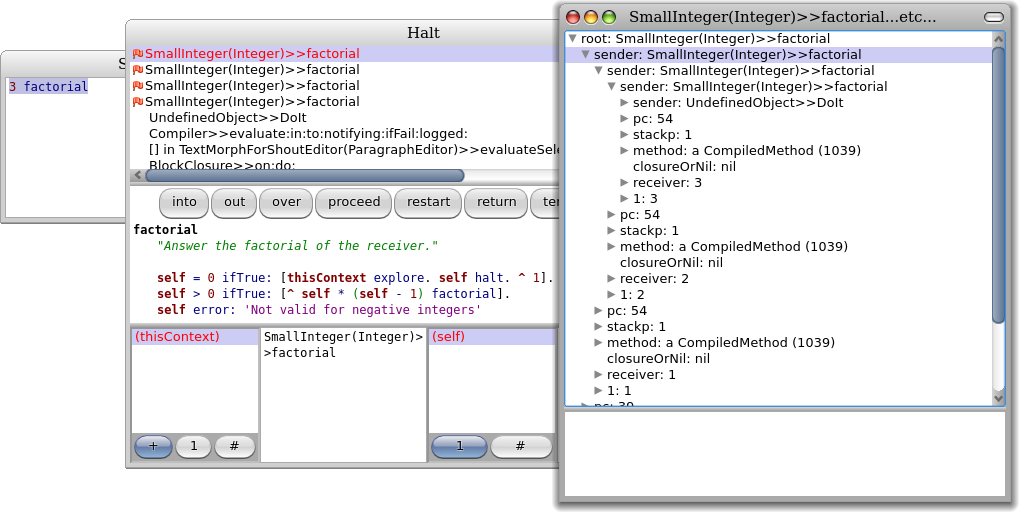
\includegraphics[width=\linewidth]{exploringThisContext}
%@	\caption{Exploring \lct{thisContext}.\figlabel{exploringThisContext}}
	\caption{\lct{thisContext}をエクスプロアしている様子。\figlabel{exploringThisContext}}
\end{figure}

%@Welcome to the poor-man's debugger!
貧者のデバッガーへようこそ!
%@If you now browse the class of the explored object (\ie by evaluating \ct{self browse} in the bottom pane of the explorer) you will discover that it is an instance of the class \lct{MethodContext}, as is each \ct{sender} in the chain.
ここでエクスプロアされたオブジェクトのクラスをブラウズすると(\ie エクスプローラーの下部のペインで\ct{self browse}を評価することによって)、\ct{thisContext}が、\lct{MethodContext}のインスタンスであることがわかるでしょう。これは、\ct{sender}の連鎖においても同様です。
% All of these objects have been created dynamically in the image by the \st virtual machine at the point where \ct{thisContext} was referred to in the \ct{factorial} method. \lr{Not actually. In all the currently available VMs the context objects are created with every method activation, no matter if they are accessed using \ct{thisContext} or not.}

%@\ct{thisContext} is not intended to be used for day-to-day programming, but it is essential for implementing tools like debuggers, and for accessing information about the call stack.
\ct{thisContext}は、日々のプログラミング用として意図されたものではありませんが、デバッガーのようなツールを実装するには不可欠であり、コールスタックについての情報にアクセスするのにも不可欠です。
%@You can evaluate the following expression to discover which methods make use of \ct{thisContext}:
以下の式を評価することにより、どのメソッドが\ct{thisContext}を活用しているかを見出すことができます:

\begin{code}{}
SystemNavigation default browseMethodsWithSourceString: 'thisContext'
\end{code}

%@As it turns out, one of the most common applications is to discover the sender of a message.
結局のところ、\ct{thisContext}の最も一般的な応用のひとつは、メッセージのセンダーを見出すことです。
%@Here is a typical application:
以下は典型的なアプリケーションです: %@?application: アプリケーションでいいか?
\begin{code}{}
Object>>>subclassResponsibility
%@	"This message sets up a framework for the behavior of the class' subclasses.
	"このメッセージは問題のクラスの一連のサブクラスの振る舞いについてのフレームワークを設定する。"
%@	Announce that the subclass should have implemented this message."
	"このメッセージがサブクラスで実装済みであるはずだ、と宣言する。"

	self error: 'My subclass should have overridden ', thisContext sender selector printString
\end{code}

%@By convention, methods in \st that send \ct{self subclassResponsibility} are considered to be abstract.  But how does \clsmthind{Object}{subclassResponsibility} provide a useful error message indicating which abstract method has been invoked?  Very simply, by asking \ct{thisContext} for the sender.
慣習により、\st のメソッドで\ct{self subclassResponsibility}を送るものは、抽象メソッドであると考えられます。しかし、\clsmthind{Object}{subclassResponsibility}メソッドは、どのようにして有用なエラーメッセージを提供するのでしょうか? つまり、どのようにして、どの抽象メソッドが呼ばれたかを示すのでしょうか? 非常に単純です。 \ct{thisContext}にセンダーを尋ねるのです。

\lr{I think co-routines and continuations should at least mentioned here. Another very practical application that is simple and could be shown here is the ``escaper''. Store the current context into a temp or inst-var \ct{target := thisContext} and jump back to that stack frame at a later point in time using \ct{target return: 123}.}
\sd{lukas maybe we should have another chapter showing such kind of beasts. I would love to read it.
Showing how to use block to build exception and such a kind of point. I think that this chapter should be an introduction may be
we should have a Reflection applied chapter}
\lr{I would love to help writing such a chapter}
%-----------------------------------------------------------------
%@\subsection{Intelligent breakpoints}
\subsection{賢いブレークポイント}

\mthindex{Object}{halt}
%@The \st way to set a breakpoint is to evaluate \ct{self halt} at an interesting point in a method.  This will cause \ct{thisContext} to be reified, and a \ind{debugger} window will open at the breakpoint.
ブレークポイントをかけるための\st のやりかたは、メソッド内の関心のある箇所で、\ct{self halt}を評価することです。こうすると、\ct{thisContext}が具現化され、\ind{デバッガー}ウィンドウが、ブレークポイントの所で開くことになります。
%@Unfortunately this poses problems for methods that are intensively used in the system.
不幸なことに、これを、システムの中核的なメソッドに対して行うと、数々の問題を引き起こすことになります。

%@Suppose, for instance, that we want to explore the execution of \ct{OrderedCollection>>>add:}.
例えば、こうしましょう。\ct{OrderedCollection>>>add:}の実行をエクスロアしたかったとしましょう。
%@Setting a breakpoint in this method is problematic.
このメソッドにブレークポイントをかけると、やっかいなことになります。

%@\dothis{Take a \emph{fresh} image and set the following breakpoint:}
\dothis{\emph{フレッシュな}仮想イメージを使って、以下のブレークポイントをセットしてみましょう:}
\needlines{3}
\begin{code}{}
OrderedCollection>>>add: newObject
	!\underline{self halt.}!
	^self addLast: newObject
\end{code}

%@Notice how your image immediately freezes!  We do not even get a debugger window.
この仮想イメージが、どのくらいただちに、フリーズするかに注目してください! デバッガーウィンドウを開けることさえできません。
%@The problem is clear once we understand that (i) \ct{OrderedCollection>>>add:} is used by many parts of the system, so the breakpoint is triggered very soon after we accept the change, but (ii) \emph{the debugger itself} sends \ct{add:} to an instance of \ct{OrderedCollection}, preventing the debugger from opening!
いったん次のことを理解すれば、問題は明確になるでしょう。(i) \ct{OrderedCollection>>>add:}はシステムの多くの場所で使われています。そして、ブレークポイントは、変更をacceptしたまさにその直後から有効になります。しかし、(ii) \emph{デバッガーそれ自身}が、\ct{add:}メッセージを\ct{OrderedCollection}のインスタンスに送るので、デバッガーを開けることができなくなるのです!
%@What we need is a way to \emph{conditionally halt} only if we are in a context of interest.
必要なのは、関心があるコンテクスト内でのみ、\emph{条件つきでhalt}する方法です。
%@This is exactly what \clsmthind{Object}{haltIf:} offers.
この方法を提供するのが、まさに、\clsmthind{Object}{haltIf:}です。

%@Suppose now that we only want to halt if \ct{add:} is sent from, say, the context of \ct{OrderedCollectionTest>>>testAdd}.
さて、haltが、何らかのコンテクスト、例えば、\ct{add:}が、\ct{OrderedCollectionTest>>>testAdd}のコンテクストから呼ばれたときにだけ起こるようにしたいとしましょう。%@?say: ?

%@\dothis{Fire up a fresh image again, and set the following breakpoint:}
\dothis{再びフレッシュな仮想イメージを立ち上げ、以下のブレークポイントを設定してみましょう:}
\begin{code}{}
OrderedCollection>>>add: newObject
	!\underline{self haltIf: \#testAdd.}!
	^self addLast: newObject
\end{code}

%@This time the image does not freeze. Try running the \ct{OrderedCollectionTest}.
今回は、仮想イメージはフリーズしません。\ct{OrderedCollectionTest}を走らせてみましょう。
%@(You can find it in the \scat{CollectionsTests-Sequenceable} category.)
\ct{OrderedCollectionTest}が、\scat{CollectionsTests-Sequenceable}カテゴリにあるのを見つけることができるでしょう。%@?くどい?

%@How does this work?  Let's have a look at \clsmthind{Object}{haltIf:}:
どうしてこのように動くのでしょうか?\clsmthind{Object}{haltIf:}の実装を見てみましょう:
\begin{code}{}
Object>>>haltIf: condition
	| cntxt |
	condition isSymbol ifTrue: [
		"only halt if a method with selector symbol is in callchain"
		cntxt := thisContext.
		[cntxt sender isNil] whileFalse: [
			cntxt := cntxt sender. 
			(cntxt selector = condition) ifTrue: [Halt signal]. ].
		^self.
	].
	...
\end{code}

%@Starting from \ct!thisContext!, \ct!haltIf:! goes up through the execution stack, checking if the name of the calling method is the same as the one passed as parameter.
\ct!thisContext!から始めて、\ct!haltIf:!は実行時スタックを上へ上へとたぐっていきながら、呼び出し側のメソッドの名前が、パラメーターとして与えられたシンボルと一致するかをチェックします。
%@If this is the case, then it raises an exception which, by default, summons the debugger.
もし一致したら、例外を発生させます。そして例外が発生したときのデフォルトの動作として、デバッガーが呼び出されます。

%@It is also possible to supply a boolean or a boolean block as an argument to \ct{haltIf:}, but these cases are straightforward and do not make use of \lct{thisContext}.
booleanやbooleanブロックを引数として、\ct{haltIf:}を呼ぶこともできますが、これらのケースについての処理は単純で、\lct{thisContext}は活用されません。

%======================================
%@\section{Intercepting messages not understood}
\section{理解されなかったメッセージをインターセプトする}
\seclabel{msgnotunderstood}

%@So far we have used the reflective features of \st mainly to query and explore objects, classes, methods and the run-time stack. Now we will look at how to use our knowledge of the \st system structure to intercept messages and modify behaviour at run-time.
これまでのところ、\st のリフレクティブな機能は、主に、オブジェクト、クラス、メソッド、そして実行時スタックにクエリを送ったり、これらをエクスプロアするのに用いてきました。ここからは、今までの\st システムの構造に関する知識をどのように使えば、メッセージをインターセプトして、その振る舞いを実行時に変えることができるか、詳しく見ていきます。

%@When an object receives a message, it first looks in the method dictionary of its class for a corresponding method to respond to the message.
オブジェクトがメッセージを受け取ったとき、オブジェクトはまず、そのクラスのメソッド辞書を引いて、メッセージに対応するメソッド、このメッセージに応答するべきメソッドを探します。
%@If no such method exists, it will continue looking up the class hierarchy, until it reaches \ct{Object}. If still no method is found for that message, the object will \emph{send itself} the message \ct{doesNotUnderstand:} with the message selector as its argument.
もし、そのようなメソッドが存在しなければ、クラス階層を上へ上へとたぐっていきます。これは場合によっては\ct{Object}にたどりつくまで続けられます。もし、そこでもメッセージに対するメソッドが見つからなかったら、オブジェクトは\emph{自分自身に} \ct{doesNotUnderstand:}を送ります。\ct{doesNotUnderstand:}の引数は、理解されなかったメッセージのメッセージセレクターです。
%@The process then starts all over again, until \clsmthind{Object}{doesNotUnderstand:} is found, and the debugger is launched.
このメソッド検索のプロセスは、振り出しに戻って再開され、\clsmthind{Object}{doesNotUnderstand:}が見つかるまで続けられ、そしてデバッガーが立ち上がります。

%@But what if \ct{doesNotUnderstand:} is overridden by one of the subclasses of \ct{Object} in the lookup path?
しかし、もし\ct{doesNotUnderstand:}が\ct{Object}のサブクラスでオーバーライドされていて、メソッドの検索パスに入っていたらどうなるでしょう?
%@As it turns out, this is a convenient way of realizing certain kinds of very dynamic behaviour. An object that does not understand a message can, by overriding \ct{doesNotUnderstand:}, fall back to an alternative strategy for responding to that message.
結局のところ、これは、ある種の非常に動的な振る舞いを理解するための、便利な方法です。あるメッセージが理解できないオブジェクトは、\ct{doesNotUnderstand:}をオーバーライドすることで、理解できないメッセージに応答するための、代替えの戦略に頼ることができるのです。%@?日本語が変

%@Two very common applications of this technique are (1) to implement \ind{lightweight proxies} for objects, and (2) to dynamically compile or load missing code.
このテクニックの非常に一般的な応用をふたつ挙げると、(1) オブジェクトの\ind{軽量プロキシー}の実装、そして、(2) 欠けているコードを動的にコンパイルまたはロードすること、です。

%-----------------------------------------------------------------
%@\subsection{Lightweight proxies}
\subsection{軽量プロキシー}

%@In the first case, we introduce a ``\ind{minimal object}'' to act as a proxy for an existing object.
最初の例として、``\ind{最低限のオブジェクト}''を紹介します。これは、既存のオブジェクトのプロキシーとして振る舞います。
%@Since the proxy will implement virtually no methods of its own, any message sent to it will be trapped by \ct{doesNotUnderstand:}. By implementing this message, the proxy can then take special action before delegating the message to the real subject it is the proxy for.
このプロキシーは実質的には、それ自身のメソッドを何ら持たないので、プロキシーに送られたどのメッセージも、\ct{doesNotUnderstand:}でトラップされます。この\ct{doesNotUnderstand:}メッセージを実装することにより、プロキシーは、それが代理を務める実体にメッセージを移譲する前に、特別なアクションを取ることができます。%@? ???

%@Let us have a look at how this may be implemented\footnote{You can also load \pkg{PBE-Reflection} from \url{http://www.squeaksource.com/PharoByExample/}}.
これが、どのように実装することができるか、見てみましょう。\footnote{\pkg{PBE-Reflection}を\url{http://www.squeaksource.com/PharoByExample/}からロードすることもできます}。

%@We define a \ct{LoggingProxy} as follows:
\ct{LoggingProxy}を以下のように定義します:
\begin{code}{}
ProtoObject subclass: #LoggingProxy
	instanceVariableNames: 'subject invocationCount'
	classVariableNames: ''
	poolDictionaries: ''
	category: 'PBE-Reflection'
\end{code}
%@Note that we subclass \ct{ProtoObject} rather than \ct{Object} because we do not want our proxy to inherit over 400 methods (!) from \ct{Object}.
\ct{Object}ではなく\ct{ProtoObject}のサブクラスとして定義していることに注意してください。なぜなら、\ct{Object}からこのプロキシーに、400個以上のメソッド(!)を継承したくないからです。

\begin{code}{}
Object methodDict size --> 408
\end{code}

%@Our proxy has two instance variables: the \ct{subject} it is a proxy for, and a \ct{count} of the number of messages it has intercepted.
このプロキシーにはふたつのインスタンス変数があります: \ct{subject} これは、このプロキシーが代理を務める実体です。そして\ct{invocationCount}は、このプロキシーがインターセプトしたメッセージの\ct{数}です。%@? ???
%@We initialize the two instance variables and we provide an accessor for the message count.
これらふたつのインスタンス変数を初期化し、インターセプトされたメッセージの数(\ct!invocationCount!)を返すアクセサを提供します。
%@Initially the \ct{subject} variable points to the proxy object itself.
最初は\ct{subject}変数は、プロキシーオブジェクトそれ自身を指しています。
\begin{code}{}
LoggingProxy>>>initialize
	invocationCount := 0.
	subject := self.
\end{code}

\begin{code}{}
LoggingProxy>>>invocationCount
	^ invocationCount
\end{code}

%@We simply intercept all messages not understood, print them to the Transcript, update the message count, and forward the message to the real subject.
理解されなかったすべてのメッセージを、単純にインターセプトし、それらをトランスクリプトに表示し、\ct!invocationCount!を更新し、そして、そのメッセージをプロキシーの実体へ転送します。
\begin{code}{}
LoggingProxy>>>doesNotUnderstand: aMessage 
	Transcript show: 'performing ', aMessage printString; cr.
	invocationCount := invocationCount + 1.
	^ aMessage sendTo: subject
\end{code}

%@Here comes a bit of magic.
ほら、ちょっとした魔法がやって来ます。%@?Here comes: 英辞郎
%@We create a new \ct{Point} object and a new \ct{LoggingProxy} object, and then we tell the proxy to \mthind{ProtoObject}{become:} the point object:
\ct{Point}オブジェクトと\ct{LoggingProxy}オブジェクトを新規に生成し、プロキシーに、\ct{Point}オブジェクトに\mthind{ProtoObject}{become:} と告げます。
\seeindex{\ct{become:}}{\ct{ProtoObject>>>become:}}
\begin{code}{}
point := 1@2.
LoggingProxy new !\underline{become:}! point.
\end{code}

%@This has the effect of swapping all references in the image to the point to now refer to the proxy, and vice versa. Most importantly, the proxy's \ct{subject} instance variable will now refer to the point!
\ct!become:!の効果は、仮想イメージの中の、この\ct{Point}オブジェクトへのすべての参照を、プロキシーへの参照とスワップし、逆に、すべてのプロキシーへの参照を、\ct{Point}オブジェクトへの参照とスワップすることです。最も重要なことですが、プロキシーの\ct{subject}インスタンス変数は、\ct{Point}オブジェクトを参照するのです!

\begin{code}{}
point invocationCount --> 0
point + (3@4)             --> 4@6
point invocationCount --> 1
\end{code}

%@This works nicely in most cases, but there are some shortcomings:
これは、多くの場合、うまく働きますが、いくつか欠点もあります:
\begin{code}{}
point class --> LoggingProxy
\end{code}
%@Curiously, the method \ct{class} is not even implemented in \ct{ProtoObject} but in \ct{Object}, which \ct{LoggingProxy} does not inherit from!
奇妙なことに、\ct{class}メソッドは、\ct{ProtoObject}で実装されてないばかりか、\ct{Object}で実装されてる\ct{class}メソッドとも違います。\ct{LoggingProxy}は、\ct{Object}を継承していません!
%@The answer to this riddle is that \ct{class} is never sent as a message but is directly answered by the virtual machine.\footnote{\ct{yourself} is also never truly sent.
この謎に対する答えは、\ct{class}はメッセージとして送られるのではなく、仮想マシンによって直接処理されるということです。\footnote{\ct{yourself}もまた、本当は、決して送られません。
%@Other messages that may be directly interpreted by the VM, depending on the receiver, include:
レシーバーが何であるかによって、直接仮想マシンが解釈することもありうるメッセージには以下のものがあります:
\ct{+- < > <= >= = ~= * / \ ==}
\ct{@ bitShift: // bitAnd: bitOr:}
\ct{at: at:put: size}
\ct{next nextPut: atEnd}
\ct{blockCopy: value value: do: new new: x y}.
%@Selectors that are never sent, because they are inlined by the compiler and transformed to comparison and jump bytecodes:
以下のセレクターは、決して送られません。なぜなら、これらはコンパイラーによって、比較とジャンプのバイトコードにインライン展開されるからです:
\ct{ifTrue: ifFalse: ifTrue:ifFalse: ifFalse:ifTrue:}
\ct{and: or:}
\ct{whileFalse: whileTrue: whileFalse whileTrue}
\ct{to:do: to:by:do:}
\ct{caseOf: caseOf:otherwise:}
\ct{ifNil: ifNotNil:  ifNil:ifNotNil: ifNotNil:ifNil:}
Attempts to send these messages to non-boolean objects can be intercepted and execution can be resumed with a valid boolean value by overriding \ct{mustBeBoolean} in the receiver or by catching the \ct{NonBooleanReceiver} exception.
}% NB: Notes by Lukas Renggli

%@Even if we can ignore such special message sends, there is another fundamental problem which cannot be overcome by this approach: \self-sends cannot be intercepted:
このような特別なメッセージ送信については、これを無視できるとしても、このアプローチでは、まだひとつ克服できない根本的な問題があります: \self-送信は、インターセプトできません:
\begin{code}{}
point := 1@2.
LoggingProxy new become: point.
point invocationCount --> 0
point rect: (3@4)        --> 1@2 corner: 3@4
point invocationCount --> 1
\end{code}

%@Our proxy has been cheated out of two \self-sends in the \ct{rect:} method:
\ct{LoggingProxy}は、\ct{rect:}メソッドの中の、ふたつの\self-送信をごまかされてしまっています: %@?has been cheated out of
\begin{code}{}
Point>>>rect: aPoint 
	^ Rectangle  origin: (self min: aPoint) corner: (self max: aPoint)
\end{code}

Although messages can be intercepted by proxies using this technique, one should be aware of the inherent limitations of using a proxy.  In \secref{wrapper} we will see another, more general approach for intercepting messages.

%-----------------------------------------------------------------
%@\subsection{Generating missing methods}
\subsection{欠けているメソッドの生成}

%@The other most common application of intercepting not understood messages is to dynamically load or generate the missing methods.
理解されなかったメッセージをインターセプトすることの、最も一般的な応用例は、欠けているメソッドの動的ロード、欠けているメソッドの動的生成です。
%@Consider a very large library of classes with many methods.  Instead of loading the entire library, we could load a stub for each class in the library. The stubs know where to find the source code of all their methods.  The stubs simply trap all messages not understood, and dynamically load the missing methods on-demand.  At some point, this behaviour can be deactivated, and the loaded code can be saved as the minimal necessary subset for the client application.
多くのメソッドからなる非常に大きなクラスライブラリについて考えてください。ライブラリ全体をロードするかわりに、各クラスのスタブをライブラリにロードすることもできるはずです。スタブは、どこを探せば、これらのすべてのメソッドのソースコードが見つかるか、ソースコードが見つかるか、を知っています。スタブは、単に、理解されなかったすべてのメッセージを捕捉し、そして、欠けているメソッドを、オンデマンドでロードします。ある時点で、この振る舞いは解除することができ、そしてロードされたコードは、クライアントアプリケーションの必要最小限のサブセットとして保存することができます。

%\on{Stef sez: check ObjectOut -- I looked, but this seems to be very old. Depends on SqueakPage.}

%@Let us look at a simple variant of this technique where we have a class that automatically adds accessors for its instance variables on-demand:
このテクニックの単純な応用例を詳しく見てみましょう。これは、オンデマンドで、自動的に、インスタンス変数へのアクセサーを追加するクラスです: %@?variant?
% \lr{the last statement should return the result of the message, otherwise you cannot proceed with the debugger} \alex{all redefinition of doesNotUnderstand: includes a return statement. However, I do not see your comment lukas, I tried to insert a 'self halt' in the method, I was able to proceed. I added the return in the function} \lr{Of course it depends on the exact circumstances. If you perform a message on self that returns self it does not matter, but in any other case a forgotten return can introduce strange side effects. There was no return in the listing below, but now there is and the problem is solved.}

\begin{code}{}
DynamicAcccessors>>>doesNotUnderstand: aMessage
	| messageName |
	messageName := aMessage selector asString.
	(self class instVarNames includes: messageName)
		ifTrue: [
			self class compile: messageName, String cr, ' ^ ', messageName.
			^ aMessage sendTo: self ].
	^ super doesNotUnderstand: aMessage
\end{code}
%@Any message not understood is trapped here. If an instance variable with the same name as the message sent exists, then we ask our class to compile an accessor for that instance variables and we re-send the message.
理解されなかったメッセージは、どれも、ここで捕捉されます。もし、送られたメッセージと同じ名前のインスタンス変数があったら、クラスに動的に生成したアクセサーのソースコードをコンパイルするように依頼します。そして、メッセージを再送信します。

%@Suppose the class \ct{DynamicAccessors} has an (uninitialized) instance variable \ct{x} but no pre-defined accessor. Then the following will generate the accessor dynamically and retrieve the value:
\ct{DynamicAccessors}クラスに、(初期化されていない)インスタンス変数\ct{x}があったにもかかわらず、事前に定義されたアクセサーがなかったとしましょう。すると以下のようにして、アクセサーが動的に生成され、そして\ct{x}の値が取り出されます。:
\needlines{2}
\begin{code}{}
myDA := DynamicAccessors new.
myDA x --> nil
\end{code}

%@Let us step through what happens the first time the message \ct{x} is sent to our object (see \figref{DynamicAccessors}).
\ct{DynamicAccessors}オブジェクトに最初に\ct{x}メッセージが送られたとき、何が起きるか、ひとつずつ見て行きましょう。(\figref{DynamicAccessors}参照).

\begin{figure}[ht]\centering
	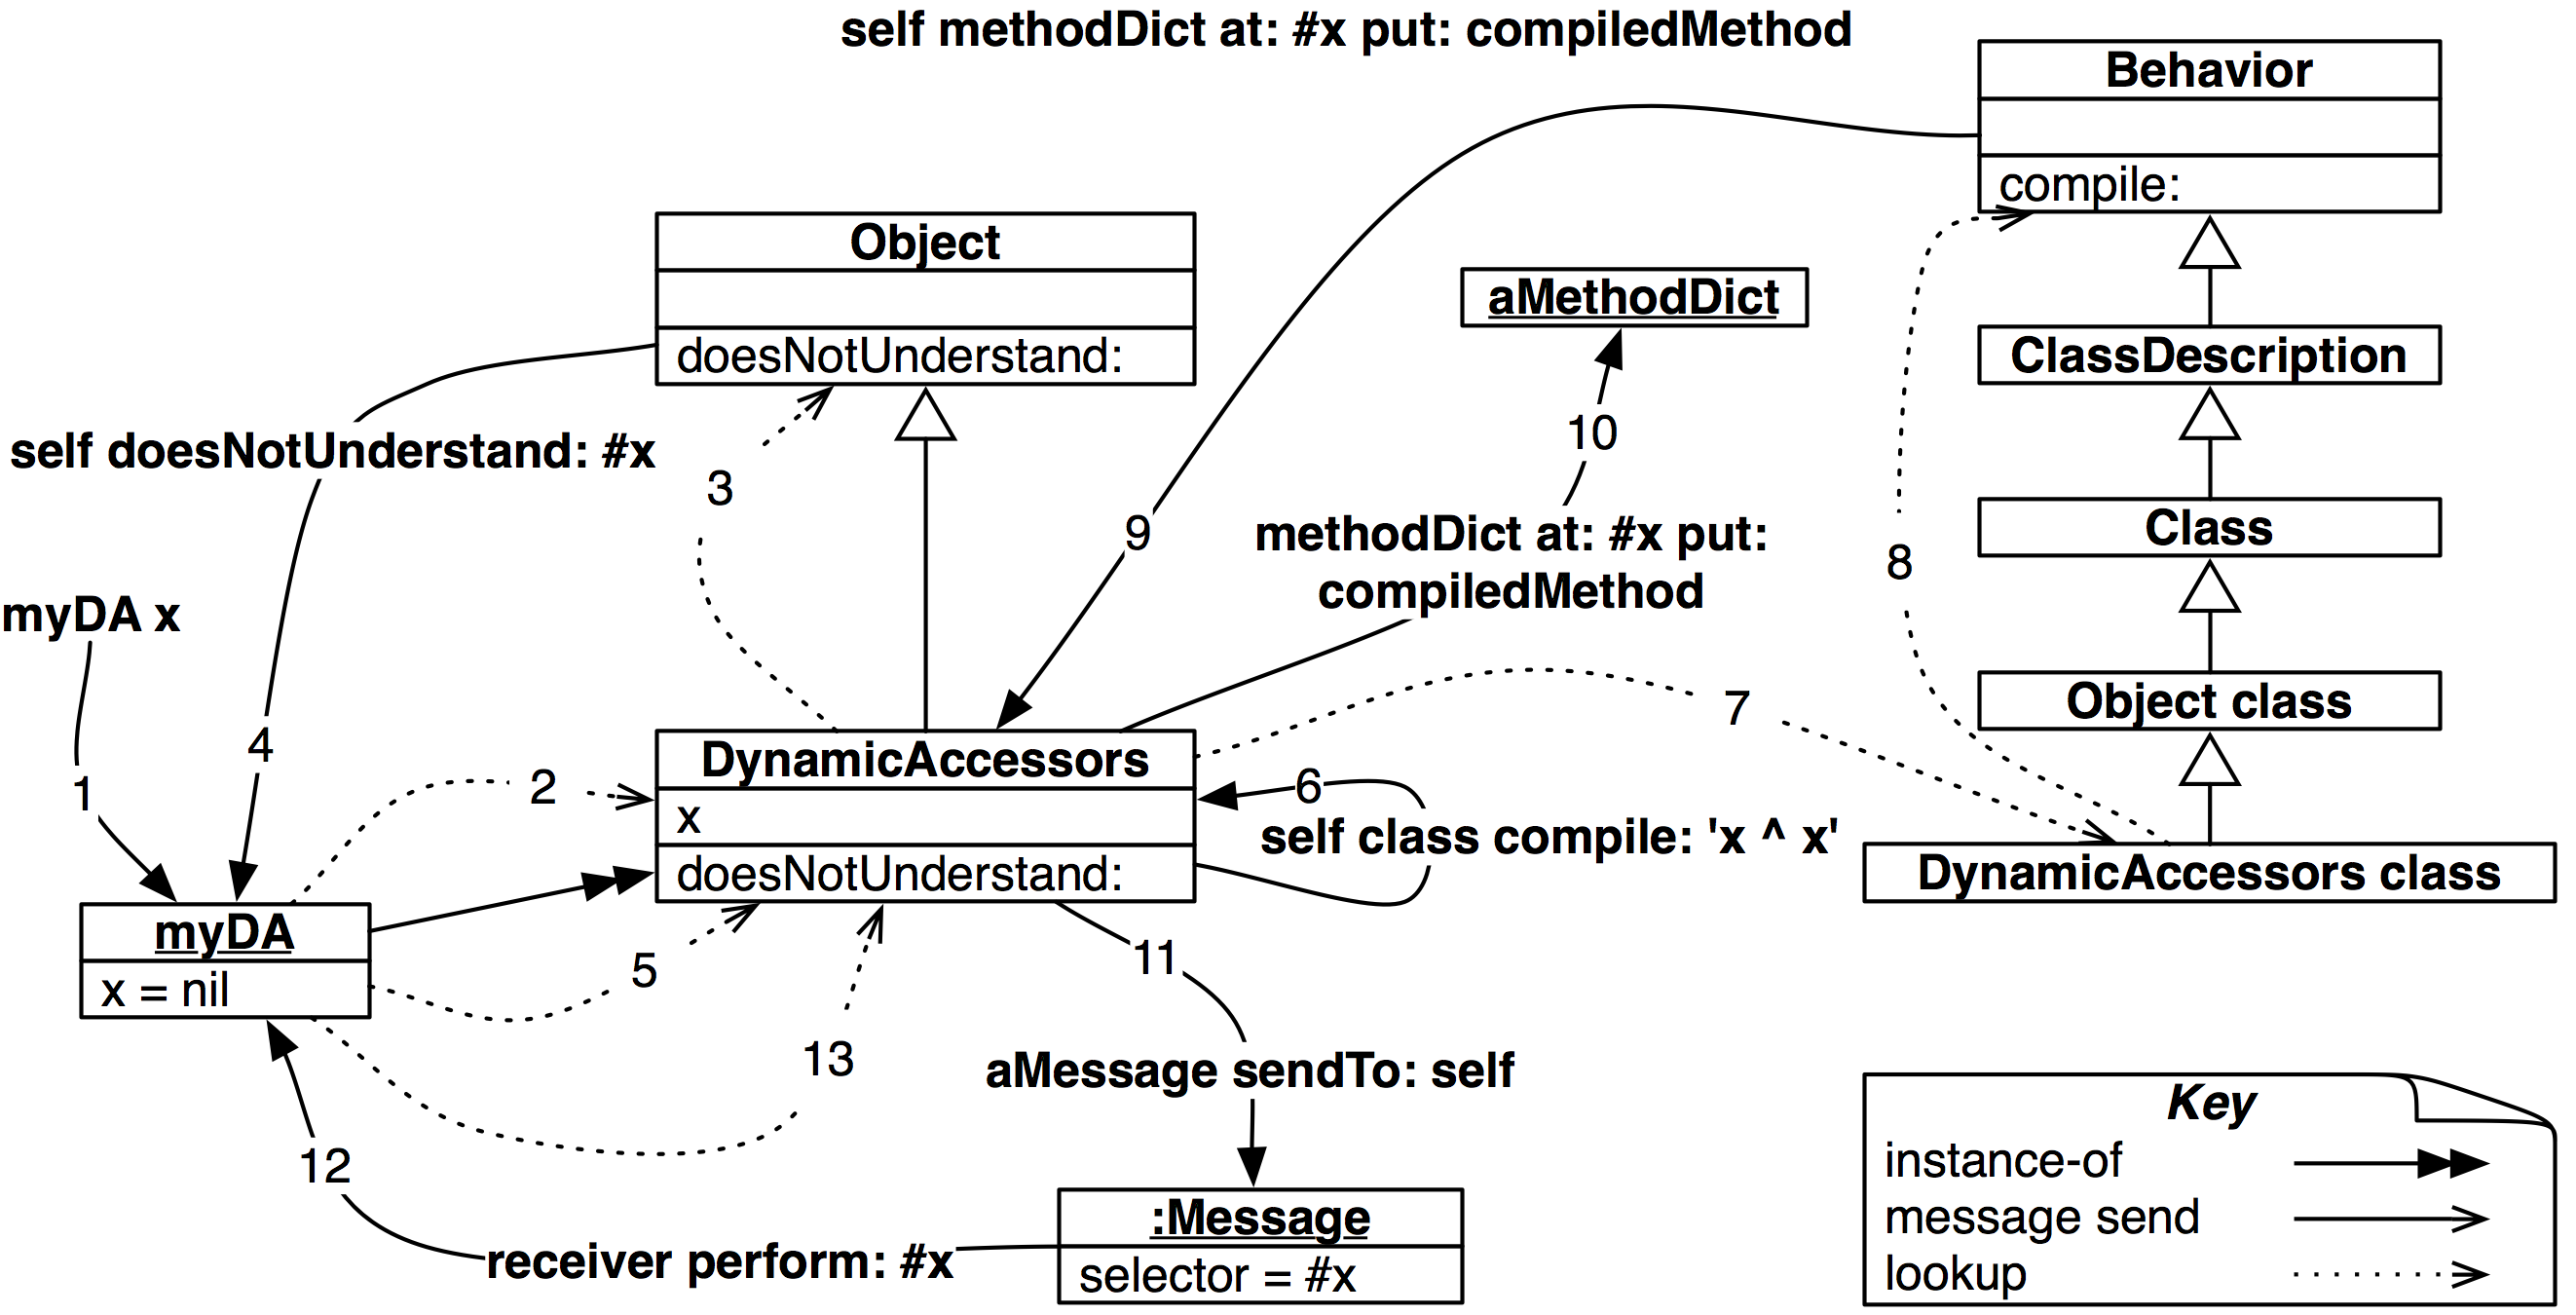
\includegraphics[width=\linewidth]{DynamicAccessors}
%@	\caption{Dynamically creating accessors.\figlabel{DynamicAccessors}}
	\caption{アクセサーの動的作成。\figlabel{DynamicAccessors}}
	% \alex{not sure whether the figure is highly necessary. The code is rather simple and the figure complete to follow in my opinion.}}
	% \on{trust me, it is useful to see all the steps.}
\end{figure}

%@(1) We send \ct{x} to \ct{myDA}, (2) the message is looked up in the class, and (3) not found in the class hierarchy. (4) This causes \ct{self doesNotUnderstand: #x} to be sent back to the object, (5) triggering a new lookup. This time \ct{doesNotUnderstand:} is found immediately in \ct{DynamicAccessors}, (6) which asks its class to compile the string \ct{'x ^ x'}. The \ct{compile} method is looked up (7), and (8) finally found in \ct{Behavior}, which (9-10) adds the new compiled method to the method dictionary of \ct{DynamicAccessors}. Finally, (11-13) the message is resent, and this time it is found.
(1) \ct{x}を\ct{myDA}に送り、(2) メッセージがクラスの中で検索され、そして、(3) クラス階層の中で見つかりません。(4) これにより、\ct{self doesNotUnderstand: #x}が、\ct{DynamicAccessors}オブジェクトに送り返され、(5) これが引き金になって、新しく検索が行われます。今度は、\ct{doesNotUnderstand:}が、ただちに\ct{DynamicAccessors}内に見つかり、(6) そして、\ct{DynamicAccessors}クラスが、文字列\ct{'x ^ x'}をコンパイルするように要求されます。\ct{compile}メソッドが検索され、(7)、そして(8) 最終的に\ct{Behavior}クラスに\ct{compile}メソッドが見つかり、それが(9-10) コンパイル済みメソッドを\ct{DynamicAccessors}のメソッド辞書に追加します。最期に、(11-13) メッセージが再送され、今度は、対応するメソッドが見つかります。

%@The same technique can be used to generate setters for instance variables, or other kinds of boilerplate code, such as visiting methods for a Visitor.
同じテクニックは、インスタンス変数のセッターや、他の種類の定型的なコード、Visitorパターンのvisitメソッドなど、を生成するのに使うことができます。v

%@Note the use of \clsmthind{Object}{perform:} in step (13) which can be used to send messages that are composed at run-time:
ステップ(13)での、\clsmthind{Object}{perform:}使い方に注意してください。\ct{perform:}メソッドを使えば、実行時に生成されたシンボルを使って、メッセージを送ることができます:
\begin{code}{@TEST}
5 perform: #factorial                                             --> 120
6 perform: ('fac', 'torial') asSymbol                       --> 720
4 perform: #max: withArguments: (Array with: 6) --> 6
\end{code}

%======================================
%@\section{Objects as method wrappers}
\section{メソッドラッパーとしてのオブジェクト}
\seclabel{wrapper}

%@We have already seen that compiled methods are ordinary objects in \st, and they support a number of methods that allow the programmer to query the run-time system.
すでに見てきたように、コンパイル済みメソッドも、\st においては、普通のオブジェクトです。そして\ct{コンパイル済みメソッドオブジェクト}にも、数々のリフレクティブなメソッドがあって、これらにより、プログラマーは実行時システムにクエリを送ることができます。
%@What is perhaps a bit more surprising, is that \emph{any object} can play the role of a compiled method. All it has to do is respond to the method \ct{run:with:in:} and a few other important messages.
少し意外なことかもしれませんが、\emph{任意のオブジェクト}は、コンパイル済みメソッドの役割の役割を担うことができます。それには、\ct{run:with:in:}メソッドと、他のいくつかの重要なメッセージに応答するだけで済みます。%@?respond to the method

%@\dothis{Define an empty class \ct{Demo}. Evaluate \ct{Demo new answer42} and notice how the usual ``Message Not Understood'' error is raised.}
\dothis{\ct{Demo}という空のクラスを定義しましょう。そして、\ct{Demo new answer42}を評価して、いつもの``Message Not Understood''エラーが引き起されるかどうかを確認しましょう。}

%@Now we will install a plain \st object in the method dictionary of our \ct{Demo} class.
さあここで、普通の\st オブジェクトを、この\ct{Demo}クラスのメソッド辞書に登録することにしましょう。

%@\dothis{Evaluate \lct{Demo methodDict at: \#answer42 put: ObjectsAsMethodsExample new.}
\dothis{\lct{Demo methodDict at: \#answer42 put: ObjectsAsMethodsExample new.}を評価しましょう。
%@Now try again to print the result of \ct{Demo new answer42}. This time we get the answer \ct{42}.}
さて、もういちど\ct{Demo new answer42}.の結果をprintしてみましょう。今度は、\ct{42}が得られます。}

%@If we take look at the class \clsind{ObjectsAsMethodsExample} we will find the following methods:
\clsind{ObjectsAsMethodsExample}を見ると、以下のメソッドが見つかるはずです:
%\alex{I would prefer having return 42 in the run:with:in: method, and not having answer42 defined in ObjectsAsMethodsExample, this could be confusing I imagine}
%\on{ObjectsAsMethodsExample is part of the standard pharo image -- it is not in PBE-Reflection}
\needlines{5}
\begin{code}{}
answer42
	^42

run: oldSelector with: arguments in: aReceiver
	^self perform: oldSelector withArguments: arguments
\end{code}

%@When our \ct{Demo} instance receives the message \ct{answer42}, method lookup proceeds as usual, however the virtual machine will detect that in place of a compiled method, an ordinary \st object is trying to play this role.
この\ct{Demo}のインスタンスが\ct{answer42}メッセージを受け取ると、メソッド検索は通常どおりに始まりますが、しかし、仮想マシンは、コンパイル済みメソッドがあるべき場所に、普通の\st のオブジェクトを検出すると、それがメソッドの代わりを務めようとしている、と判断します。%@?意訳しすぎか?
%@The VM will then send this object a new message \ct{run:with:in:} with the original method selector, arguments and receiver as arguments.
VMは、このオブジェクトに、\ct{run:with:in:}というメッセージを送り、このとき、もともとのメソッドセレクターと、もともとの引数と、レシーバーが、\ct{run:with:in:}の引数になります。%@?will: 無視した。VM: マクロ化しないのか?
%@Since \ct{ObjectsAsMethodsExample} implements this method, it intercepts the message and delegates it to itself.
\ct{ObjectsAsMethodsExample}は、この\ct{run:with:in:}メソッドを実装しているので、これはメッセージをインターセプトして、自分自身にメッセージを移譲します。

%@We can now remove the fake method as follows:
ここで、このためのメソッドは、以下のようにして、削除することができます:
\begin{code}{}
Demo methodDict removeKey: #answer42 ifAbsent: []
\end{code}

%@If we take a closer look at \ct{ObjectsAsMethodsExample}, we will see that its superclass also implements the methods \ct{flushcache}, \ct{methodClass:} and \lct{selector:}, but they are all empty.  These messages may be sent to a compiled method, so they need to be implemented by an object pretending to be a compiled method.  (\ct{flushcache} is the most important method to be implemented; others may be required depending on whether the method is installed using \clsmthind{Behavior}{addSelector:withMethod:} or directly using \clsmthind{MethodDictionary}{at:put:}.)
\ct{ObjectsAsMethodsExample}をよく見ると、そのスーパークラスがまた、\ct{flushcache}、\ct{methodClass:}、そして\lct{selector:}といったメソッドを定義しており、しかし、それらはすべて空になっていることがわかります。これらのメッセージは、コンパイル済みメソッドに送られる可能性があるので、コンパイル済みメソッドを装うオブジェクト、以上のメソッドを実装していなければいけません。(実装すべき最も重要なメソッドは\ct{flushcache}で; 他のメソッドは、場合によって必要となる可能性があります。つまり、そのメソッドが\clsmthind{Behavior}{addSelector:withMethod:}を使ってインストールされたのか、あるいは、\clsmthind{MethodDictionary}{at:put:}を使って直接インストールされたのか) %@? ???

%-------------------------------------------------------------------------
%@\subsection{Using method wrappers to perform test coverage}
\subsection{メソッドラッパーを、テストカバレッジの測定に使う}

%@Method wrappers are a well-known technique for intercepting messages \cite{Bran98a}.
メソッドラッパーは、メッセージをインターセプトするための、よく知られたテクニックです\cite{Bran98a}。
%@In the original implementation\footnote{http://www.squeaksource.com/MethodWrappers.html}, a method wrapper is an instance of a subclass of \ct{CompiledMethod}. When installed, a method wrapper can perform special actions before or after invoking the original method.
もともとの実装\footnote{http://www.squeaksource.com/MethodWrappers.html}では、メソッドラッパーとして、\ct{CompiledMethod}のサブクラスのインスタンスを使います。インストールされるとメソッドラッパーは、もともとのメソッドを呼び出す前かあとに、特別なアクションを実行することができます。
%@When uninstalled, the original method is returned to its rightful position in the method dictionary.
アンインストールされると、もともとのメソッドは、メソッド辞書内の、本来あるべき位置に戻されます。

%@In Pharo, \ind{method wrappers} can be implemented more easily by implementing \ct{run:with:in:} instead of by subclassing \ct{CompiledMethod}. In fact, there exists a lightweight implementation of objects as method wrappers\footnote{http://www.squeaksource.com/ObjectsAsMethodsWrap.html}, but it is not part of standard Pharo at the time of this writing.
Pharoでは、\ind{メソッドラッパー}は、\ct{CompiledMethod}をサブクラスするかわりに、\ct{run:with:in:}を実装すればよく、より簡単に実装することができます。実際、オブジェクトによる軽量のメソッドラッパーの実装\footnote{http://www.squeaksource.com/ObjectsAsMethodsWrap.html}が存在します。しかし、これを書いている時点では、この実装は、標準のPharoの一部ではありません。

%@Nevertheless, the Pharo Test Runner uses precisely this technique to evaluate test coverage.
にもかかわらず、Pharoのテストランナーは、カバレッジを評価するのに、まさにこのテクニックを使っています。
%@Let's have a quick look at how it works.
テストランナーがどのように動作するか、ザッと見てみましょう。

%@The entry point for test coverage is the method \clsmthind{TestRunner}{runCoverage}:
テストカバレッジのエントリーポイントは、\clsmthind{TestRunner}{runCoverage}です:
\begin{code}{}
TestRunner>>>runCoverage
	| packages methods |
%@	... "identify methods to check for coverage"
	... "カバレッジを測定するメソッドを識別する" %@? ???
	self collectCoverageFor: methods
\end{code}

%@The method \clsmthind{TestRunner}{collectCoverageFor:} clearly illustrates the coverage checking algorithm:
この\clsmthind{TestRunner}{collectCoverageFor:}メソッドは、カバレッジチェックのアルゴリズムを、明瞭に説明しています:
\begin{code}{}
TestRunner>>>collectCoverageFor: methods
	| wrappers suite |
	wrappers := methods collect: [ :each | TestCoverage on: each ].
	suite := self
		reset;
		suiteAll.
	[ wrappers do: [ :each | each install ].
	  [ self runSuite: suite ] ensure: [ wrappers do: [ :each | each uninstall ] ] ] valueUnpreemptively.
	wrappers := wrappers reject: [ :each | each hasRun ].
	wrappers isEmpty 
		ifTrue: 
			[ UIManager default inform: 'Congratulations. Your tests cover all code under analysis.' ]
		ifFalse: ...
\end{code}
%@A wrapper is created for each method to be checked, and each wrapper is installed.
チェックする各メソッドについて1個ずつラッパーが作られ、そして、各ラッパーがインストールされます。
%@The tests are run, and all wrappers are uninstalled.
テストが実行され、すべてのラッパーはアンインストールされます。
%@Finally the user obtains feedback concerning the methods that have not been covered.
最後に、カバーされなかったメソッドについてのフィードバックが、得られます。

%@How does the wrapper itself work?
ラッパーそれ自身は、どのように動くのでしょうか?
%@The \ct{TestCoverage} wrapper has three instance variables, \ct{hasRun}, \ct{reference} and \ct{method}.
次の\ct{TestCoverage}ラッパーには、3個のインスタンス変数: \ct{hasRun}、\ct{reference}、\ct{method}があります。
%@They are initialized as follows:
これらは以下のように初期化されます。
\begin{code}{}
TestCoverage class>>>on: aMethodReference
	^ self new initializeOn: aMethodReference

TestCoverage>>>initializeOn: aMethodReference
	hasRun := false.
	reference := aMethodReference.
	method := reference compiledMethod
\end{code}

%@The install and uninstall methods simply update the method dictionary in the obvious way:
installメソッドと、uninstallメソッドは、自明な方法で、メソッド辞書を更新します:
\begin{code}{}
TestCoverage>>>install
	reference actualClass methodDictionary
		at: reference methodSymbol
		put: self

TestCoverage>>>uninstall
	reference actualClass methodDictionary
		at: reference methodSymbol
		put: method
\end{code}
\noindent
%@and the \ct{run:with:in:} method simply updates the \ct{hasRun} variable, uninstalls the wrapper (since coverage has been verified), and resends the message to the original method
そして、\ct{run:with:in:}メソッドは、単に、\ct{hasRun}インスタンス変数を更新し、ラッパー(それ自身)をアンインストールし(カバレッジが検証されたから)、もともとのメソッドにメッセージを再送します。%@?resends the message to the original method?
\begin{code}{}
run: aSelector with: anArray in: aReceiver
	self mark; uninstall.
	^ aReceiver withArgs: anArray executeMethod: method

mark
	hasRun := true
\end{code}
%@(Have a look at \clsmthind{ProtoObject}{withArgs:executeMethod:} to see how a method displaced from its method dictionary can be invoked.)
テ(Have a look at \clsmthind{ProtoObject}{withArgs:executeMethod:} to see how a method displaced from its method dictionary can be invoked.)

%@That's all there is to it!
ただそれだけのことです。

%@Method wrappers can be used to perform any kind of suitable behaviour before or after the normal operation of a method.  Typical applications are instrumentation (collecting statistics about the calling patterns of methods), checking optional pre- and post-conditions, and memoization (optionally cacheing computed values of methods).
メソッドラッパーを使えば、あらゆる種類の振る舞いを(それが適切であれば)、通常のメソッドの操作の前後に実行させることができます。典型的な応用例は、インストゥルメンテーション(メソッドの呼び出しパターンに関する統計を収集すること)、オプションの、事前・事後条件のチェック、 メモイゼーション(オプションで、メソッドが計算した値をキャッシュすること)です。

%======================================
%@\section{Pragmas}
\section{プラグマ}

%@A \emphind{pragma} is an annotation that specifies data about a program, but is not involved in the execution of the program. Pragmas have no direct effect on the operation of the method they annotate.
\emphind{プラグマ}は、プログラムについてのデータについて詳細に述べるためのアノテーション(注釈)ですが、プログラムの実行には関与しません。プラグマは、それらがアノテートするメソッドの操作に、直接影響しません。
%@Pragmas have a number of uses, among them:
プラグマには、いくつもの使い道があります、それらは、例えば以下のようなものです:
\begin{itemize}
%@\item Information for the compiler: \indmain{pragmas} can be used by the compiler to make a method call a primitive function. This function has to be defined by the virtual machine or by an external plug-in.
\item コンパイラーへの情報: \indmain{プラグマ}は、コンパイラがメソッド呼び出しをプリミティブ関数にするのに用いられます。このプリミティブ関数は、バーチャルマシンか外部プラグインが定義しなければなりません。
%@\item Runtime processing: Some pragmas are available to be examined at runtime.
\item 実行時処理: いくつかのプラグマは、実行時にこれを検査することができます。%@?プログラムの実行には関与しないのではなかったか?
\end{itemize}

%@Pragmas can be applied to a program's method declarations only. A method may declare one or more pragmas, and the pragmas have to be declared prior any Smalltalk statement. Each pragma is in effect a static message send with literal arguments.
プラグマが適用可能なのは、プログラムのメソッド宣言においてのみです。メソッドは、1個かそれ以上のプラグマを宣言することができ、そしてプラグマは、どのSmalltalkの文よりも先に宣言されなければなりません。各プラグマは、事実上、リテラル引数をともなった静的メッセージ送信です。

%@We briefly saw pragmas when we introduced primitives earlier in this chapter. A primitive is nothing more than a pragma declaration. 
この章の最初の方でプリミティブを紹介したときに、簡単なプラグマの例を見ました。プリミティブは、プラグマ宣言以上のなにものでもありません。 
%@Consider \ct{<primitive: 73>} as contained in \ct{instVarAt:}. The pragma's selector is \ct{primitive:} and its arguments is an immediate literal value, \ct{73}. 
\ct{instVarAt:}メソッドの定義内の\ct{<primitive: 73>}を検討してください。このプラグマのセレクターは、\ct{primitive:}であり、その引数はリテラル値で、\ct{73}です。%@?immediate: 訳さなかった。

%@The compiler is probably the bigger user of pragmas. SUnit is another tool that makes use of annotations. SUnit is able to estimate the coverage of an application from a test unit. One may want to exclude some methods from the coverage. This is the case of the \ct!documentation! method in \ct!SplitJointTest class!:
コンパイラーはおそらく、プラグマの大口ユーザです。SUnitもまた、アノテーションを活用するツールです。SUnitは、テストユニットからアプリケーションのカバレッジを見積ることができます。いくつかのメソッドを、カバレッジから除外したいと思うかもしれません。以下は、\ct!SplitJointTest class!の\ct!documentation!メソッドの場合です:

\begin{code}{}
SplitJointTest class>>>documentation
	<ignoreForCoverage>
	"self showDocumentation"
	
	^ 'This package provides function.... "
\end{code}

%@By simply annotating a method with the pragma \ct!<ignoreForCoverage>! one can control the scope of the coverage.
このように単に、メソッドを\ct!<ignoreForCoverage>!プラグマでアノテートするだけで、カバレッジの範囲をコントロールすることができます。

%Beside the compiler, Lint is a heavy user of pragmas. Lint is a static code analyzer that flags suspicious, non-portable constructs and code that is likely to contain bugs. It may happen that a method needs to be excluded from Lint analysis. This is the case here:

%\begin{code}{}
%MorphObjectOut>>>doesNotUnderstand: aMessage 
%	"Bring in the object, install, then resend aMessage"
%	"Transcript show: thisContext sender selector; cr."
%	"useful for debugging"
%	
%	! \textbf{<lint: 'Unnecessary "= true"' rationale: 'recursionFlag may be nil' author: 'stephane.ducasse'>}!
%	...
%\end{code}	

%One of the pragmas used by Lint to filter out methods is \ct{lint:rationale:author:}.

%@As instances of the class \clsind{Pragma}, pragmas are first class objects. A compiled method answers to the message \mthind{CompiledMethod}{pragmas}. This method returns an array of pragmas. 
プラグマは、\clsind{Pragma}のインスタンスであって、ファーストクラスのオブジェクトです。コンパイル済みメソッドは、\mthind{CompiledMethod}{pragmas}メッセージに答えます。この\ct!pragmas!メソッドは、プラグマの配列を返します。

\begin{code}{}
(SplitJoinTest class >> #showDocumentation) pragmas.
  --> an Array(<ignoreForCoverage>)
(Float>>#+) pragmas --> an Array(<primitive: 41>)
\end{code}

%@Methods defining a particular query may be retrieved from a class. The class side of \ct!SplitJoinTest! contains some methods annotated with \ct!<ignoreForCoverage>!:
特定のクエリを定義するメソッドが、クラスから取り出されることがあり得ます。\ct!SplitJoinTest!のクラス側には、\ct!<ignoreForCoverage>!とアノテートされた、いくつかのメソッドがあります: %@!retrieved: ???

\begin{code}{@TEST}
Pragma allNamed: #ignoreForCoverage in: SplitJoinTest class  --> an Array(<ignoreForCoverage> <ignoreForCoverage> <ignoreForCoverage>)
\end{code}

%@A variant of \ct{allNamed:in:} may be found on the class side of \ct{Pragma}.
\ct{allNamed:in:}の変種が、\ct{Pragma}のクラス側に見付かるでしょう。

%@A pragma knows in which method it is defined (using \ct{method}), the name of the method (\ct{selector}), the class that contains the method (\ct{methodClass}), its number of arguments (\ct{numArgs}), about the literals the pragma has for arguments (\ct{hasLiteral:} and \ct{hasLiteralSuchThat:}). 
プラグマは、どのメソッドの中で、そのプラグマが定義されたか知っていおり(\ct{method}を使えばわかります)、そのメソッドの名前を(\ct{selector})、そのメソッドを含むクラスを(\ct{methodClass})、プラグマの引数の数を(\ct{numArgs})、プラグマに特定の引数リテラルがあるかどうかを(\ct{hasLiteral:}そして\ct{hasLiteralSuchThat:})知っています。 

\lr{Typically pragmas are performed on an interpreter object that understands the pragma message.}

%======================================
%@\section{Chapter summary}
\section{章のまとめ}

%@Reflection refers to the ability to query, examine and even modify the metaobjects of the run-time system as ordinary objects.
リフレクションと言った場合、それは、実行時システムのメタオブジェクトについて、これにクエリを送ることができたり、これが分析できたり、これを変更することさえできたりすることを指します。こうした点で、メタオブジェクトは、普通のオブジェクトと同等です。

\begin{itemize}
%@\item The Inspector uses \ct{instVarAt:} and related methods to query and modify ``private'' instance variables of objects.
\item インスペクターは、\ct{instVarAt:}や、関連するメソッドを用いて、オブジェクトの``プライベート''なインスタンス変数にクエリを送ったり、これを変更したりします。
%@\item Send \ct{Behavior>>>allInstances} to query instances of a class.
\item与えられたクラスの(すべての)インスタンス知りたければ、\ct{Behavior>>>allInstances}をそのクラスに送りましょう。
%@\item The messages \ct{class}, \ct{isKindOf:}, \ct{respondsTo:} \etc  are useful for gathering metrics or building development tools, but they should be avoided in regular applications: they violate the encapsulation of objects and make your code harder to understand and maintain.
\item ct{class}、\ct{isKindOf:}、\ct{respondsTo:} \etc メソッドは、メトリクスを収集したり、開発ツールを構築するのには便利ですが、通常のアプリケーションでは、これらを使うことは避けるべきです: これらのメソッドはオブジェクトのカプセル化の原則に反し、コードを理解しづらく、保守しづらいものにします。
%@\item \ct{SystemNavigation} is a utility class holding many useful queries for navigation and browsing the class hierarchy. For example, use \ct{SystemNavigation default browseMethodsWithSourceString: 'pharo'.} to find and browse all methods with a given source string. (Slow, but thorough!)
\item \ct{SystemNavigation} はユーティリティークラスであって、クラス階層をナビゲートし、ブラウズするのに、便利なクエリを備えています。例えば、任意の文字列をソースコードに含む、すべてのメソッドを見つけ出すには、\ct{SystemNavigation default browseMethodsWithSourceString: 'pharo'.}を使いましょう。(遅いですが、完全な方法です!)
%@\item Every \st class points to an instance of \ct{MethodDictionary} which maps selectors to instances of \ct{CompiledMethod}. A compiled method knows its class, closing the loop.
\item どの \st クラスにも、\ct{MethodDictionary}があって、この辞書は、セレクターとコンパイル済みメソッドのインスタンスを対応づけています。コンパイル済みメソッドは、そのクラスを知っています。こうして、両者はお互いのことを知っていることになります。
%@\item \ct{MethodReference} is a leightweight proxy for a compiled method, providing additional convenience methods, and used by many \st tools. 
\item \ct{MethodReference}は、コンパイル済みメソッドの軽量プロキシーです。\ct{MethodReference}は、追加の簡便メソッドを提供しするもので、多くの\st ツールが、この\ct{MethodReference}を使っています。
%@\item \ct{BrowserEnvironment}, part of the Refactoring Browser infrastructure, offers a more refined interface than \ct{SystemNavigation} for querying the system, since the result of a query can be used as a the scope of a new query. Both GUI and programmatic interfaces are available.
\item \ct{BrowserEnvironment}、これはリファクタリングブラウザのインフラの一部ですが、これによって、\ct{SystemNavigation}より洗練されたインターフェースでもって、システムにクエリを送ることができます。クエリの結果が、次の新しいクエリのスコープとして使えるからです。GUIによるインターフェースとプログラム的なインターフェースの両方が利用できます。%@?scope: カタカナのままにした。
%@\item \ct{thisContext} is a pseudo-variable that reifies the run-time stack of the virtual machine. It is mainly used by the debugger to dynamically construct an interactive view of the stack. It is also especially useful for dynamically determining the sender of a message.
\item \ct{thisContext}疑似変数です。この疑似変数は、仮想マシンの実行時スタックを具現化したものです。\ct{thisContext}は、主にデバッガーで使われ、スタックの会話的なビューを動的に構築するのに使われます。\ct{thisContext}はまた、メッセージのセンダーを動的に特定したい場合に、とりわけ便利です。%@?したい場合に: 意訳しすぎか?
%@\item Intelligent breakpoints can be set using \ct{haltIf:}, taking a method selector as its argument. \ct{haltIf:} halts only if the named method occurs as a sender in the run-time stack.
\item \ct{haltIf:}を使えば、賢いブレークポイントを設定することができます。このとき、メソッドセレクターを、\ct{haltIf:}の引数にします。\ct{haltIf:}は、その引数が示すメソッドが、センダーとして、実行時スタック内に現われたときのみ、停止します。
%@\item A common way to intercept messages sent to a given target is to use a ``minimal object'' as a proxy for that target. The proxy implements as few methods as possible, and traps all message sends by implementing \ct{doesNotunderstand:}. It can then perform some additional action and then forward the message to the original target.
\item 一般的には、与えられたターゲットに送られるメッセージをインターセプトするには、``最低限のオブジェクト''を使います。最低限のオブジェクトは、ターゲットのプロキシーにします。プロキシーで実装するメッセージは、できるだけ少なくします。そして、\ct{doesNotunderstand:}を実装して、すべてのメッセージを捕捉します。こうすれば、もともとのターゲットにメッセージを転送する前後に、ある種の追加のアクションを実行することができます。%@?「前後に」なんて書いていない
%@\item Send \ct{become:} to swap the references of two objects, such as a proxy and its target.
\item ふたつのオブジェクト参照を交換するには、\ct{become:}を使いましょう。\ct{become:}は、プロキシーとそのターゲットを交換するのに使えます。
%@\item Beware, some messages, like \ct{class} and \ct{yourself} are never really sent, but are interpreted by the VM.  Others, like \ct{+}, \ct{-} and \ct{ifTrue:} may be directly interpreted or inlined by the VM depending on the receiver.
\item 注意してください。いくつかのメッセージ、例えば\ct{class}や\ct{yourself}は、決して実際には送られず、代わりに、VMによって捕捉されます。他の、例えば、\ct{+}, \ct{-} and \ct{ifTrue:} も、直接VMによって解釈されるか、インライン展開されます。このようなことが起こるかどうかは、レシーバーによって異なります。%@?VMがインライン展開する?
%@\item Another typical use for overriding \ct{doesNotUnderstand:} is to lazily load or compile missing methods.
\item \ct{doesNotUnderstand:}をオーバーライドする、典型的な例としては、欠けているメソッドの遅延ロードまたは遅延コンパイルです。
%@\item \ct{doesNotUnderstand:} cannot trap \self-sends.
\item \ct{doesNotUnderstand:}は、\self-送信を捕捉することはできません。
%@\item A more rigorous way to intercept messages is to use an object as a method wrapper. Such an object is installed in a method dictionary in place of a compiled method. It should implement \ct{run:with:in:} which is sent by the VM when it detects an ordinary object instead of a compiled method in the method dictionary. This technique is used by the SUnit Test Runner to collect coverage data.
\item オブジェクトをメソッドラッパーとして使えば、より厳密な意味で、メッセージをインターセプトすることができます。このようなラッパーは、メソッド辞書内の、本来ならコンパイル辞書が格納されるべき場所にインストールされます。ラッパーは、\ct{run:with:in:}を実装しなければなりあせん。このメッセージは、VMが、メソッド辞書内で、コンパイル済みメソッドの代わりに普通のオブジェクトを検出したときに送られます。このテクニックは、SUnitテストランナーが、カバレッジデータを収集するのに使われています。%@?意訳しすぎか?
\end{itemize}

%=========================================================
\ifx\wholebook\relax\else
   \bibliographystyle{jurabib}
   \nobibliography{scg}
   \end{document}
\fi
%=========================================================

%Other stuff:
%- anonymous classes (uses compile: and primitiveChangeClassTo:) ???
%- collect direct senders; class collaborations
%- Object primitiveChangeClassTo: become: and becomeForward: (see tests and slides with minimal object example)
%- PointerFinder?
%- anonymous classes (see slides) ?

%Test  Coverage using ObjectsAsMethodsWrap package:
%\begin{code}{}
%category := 'SCGPier'.
%w := (ObjectAsOneTimeMethodWrapper installOnClassCategory: category).
%tr := TestRunner new.
%ToolBuilder open: tr.
%[tr
%	categoryAt: (tr categoryList indexOf: 'SCGPier') put: true;
%	selectAllClasses;
%	runAll.]
%ensure: [[w do: [:each| each uninstall ]] valueUnpreemptively].
%((w select: [:each | each executed not ])
%	collect: [:each | each wrappedClass name, '>>', each selector name ]) explore.
%\end{code}
